\documentclass[11pt,openany]{article}

\input{ca-preamble}
\usepackage{tcolorbox}
\tcbset{colback=white, arc=5pt}

\definecolor{axiomcolor}{HTML}{a88bfa}
\definecolor{defcolor}{RGB}{52, 152, 219}
\definecolor{procolor}{RGB}{241, 196, 15}
\definecolor{thmcolor}{RGB}{231, 76, 60}
\definecolor{lemcolor}{RGB}{155, 89, 182}
\definecolor{corcolor}{RGB}{46, 204, 113}
\definecolor{execolor}{RGB}{90, 128, 127}

% Define a new command for the custom tcolorbox
\newcommand{\axiombox}[2][]{%
	\begin{tcolorbox}[colframe=axiomcolor, title={\color{white}\bfseries #1}]
		#2
	\end{tcolorbox}
}

\newcommand{\defbox}[2][]{%
	\begin{tcolorbox}[colframe=defcolor, title={\color{white}\bfseries #1}]
		#2
	\end{tcolorbox}
}

\newcommand{\probox}[2][]{%
	\begin{tcolorbox}[colframe=procolor, title={\color{white}\bfseries #1}]
		#2
	\end{tcolorbox}
}

\newcommand{\thmbox}[2][]{%
	\begin{tcolorbox}[colframe=thmcolor, title={\color{white}\bfseries #1}]
		#2
	\end{tcolorbox}
}

\newcommand{\lembox}[2][]{%
	\begin{tcolorbox}[colframe=lemcolor, title={\color{white}\bfseries #1}]
		#2
	\end{tcolorbox}
}
\usepackage{amsthm}

% Define custom theorem styles
\newtheoremstyle{dotless} % Name of the style
{3pt} % Space above
{3pt} % Space below
{\itshape} % Body font
{} % Indent amount
{\bfseries} % Theorem head font
{} % Punctuation after theorem head
{2.5mm} % Space after theorem head
{} % Theorem head spec

\newtheoremstyle{definitionstyle} % Name of the style
{3pt} % Space above
{3pt} % Space below
{} % Body font
{} % Indent amount
{\bfseries} % Theorem head font
{.} % Punctuation after theorem head
{2.5mm} % Space after theorem head
{} % Theorem head spec

% Applying custom styles
%\theoremstyle{dotless}
\newtheorem{theorem}{Theorem} % Theorem environment with section-wise numbering
\newtheorem*{theorem*}{Theorem} % Theorem environment with section-wise numbering
\newtheorem*{lemma*}{Lemma} % Theorem environment with section-wise numbering
\newtheorem*{proposition*}{Proposition} % Theorem environment with section-wise numbering
\newtheorem*{corollary*}{Corollary} % Theorem environment with section-wise numbering
\newtheorem{proposition}[theorem]{Proposition} % Theorem environment with section-wise numbering
\newtheorem{lemma}[theorem]{Lemma} % Lemma shares the counter with theorem
\newtheorem{corollary}[theorem]{Corollary} % Corollary shares the counter with theorem

\theoremstyle{definitionstyle}
\newtheorem*{observation}{\textcolor{magenta}{Observation}}
\newtheorem*{illustration}{\textcolor{teal}{Illustration}}
\newtheorem*{torus}{{\color{red}T}{\color{orange}o}{\color{green!75!black}r}{\color{cyan}u}{\color{violet}s}}
\newtheorem{definition}{Definition} % Definition shares the counter with theorem
\newtheorem{example}{Example} % Example shares the counter with theorem
\newtheorem{exercise}{{Exercise}} % Example shares the counter with theorem
\newtheorem{remark}{Remark} % Remark shares the counter with theorem
\newtheorem*{note}{Note}
\newtheorem*{notation}{Notation}

\newtheorem*{axiom*}{Axiom}
\newtheorem*{definition*}{Definition} % Definition shares the counter with theorem
\newtheorem*{example*}{Example} % Example shares the counter with theorem
\newtheorem*{exercise*}{\textcolor{teal}{Exercise}} % Example shares the counter with theorem
\newtheorem*{remark*}{Remark} % Remark shares the counter with theorem


\usepackage{tikz}
\usepackage{tikz-cd}
\usetikzlibrary{shadows}
\usetikzlibrary{shapes.geometric, arrows.meta, positioning}
\input{ca-commands}
\renewcommand{\Re}{\mathrm{Re}}
\renewcommand{\Im}{\mathrm{Im}}
\renewcommand{\vec}[1]{\mathbf{#1}}
\renewcommand{\emph}[1]{\textbf{#1}}
\renewcommand{\d}{\mathrm{d}} % For the exterior derivative 'd'
\newcommand{\pderiv}[2]{\frac{\partial #1}{\partial #2}}
\newcommand{\spderiv}[3]{\frac{\partial^2 #1}{\partial #2\partial #3}}
\newcommand{\vect}[1]{\begin{bmatrix} #1 \end{bmatrix}}

\renewcommand{\Re}{\operatorname{\mathrm{Re}}}
\renewcommand{\Im}{\operatorname{\mathrm{Im}}}

\newcommand{\circulationsquare}[1]{
	\draw[thick, gray] #1 rectangle ++(1,1);
	\begin{scope}[decoration={markings, mark=at position 0.5 with {\arrow{>}}}]
		\draw[postaction={decorate}, blue] #1 -- ++(1,0);
		\draw[postaction={decorate}, blue] ++(1,0) -- ++(0,1);
		\draw[postaction={decorate}, blue] ++(0,1) -- ++(-1,0);
		\draw[postaction={decorate}, blue] ++(-1,0) -- cycle;
	\end{scope}
}

\newcommand{\Sol}{{\color{magenta}\normalfont\bfseries\text{Sol}}}

\usepackage{esvect}
\usepackage{physics}

\setstretch{1.25}

\begin{document}
\pagenumbering{arabic}
\begin{center}
	\huge\textbf{Complex Analysis}\\
	\vspace{0.5em}
	\large{Ji, Yong-hyeon}\\
	\vspace{0.5em}
	\normalsize{\today}\\
\end{center} 
\tableofcontents
\vspace{1em}

\newpage
\section{Complex Numbers}

\subsection{Complex Numbers}

\begin{definition}[Complex numbers and parts]
	A complex number is an ordered pair $(x,y)\in\R^2$, denoted $z=(x,y)$ or $z=x+iy$, with \emph{real part} $\Re z=x$ and \emph{imaginary part} $\Im z=y$.
\end{definition}

\begin{remark}
	Two complex numbers are equal iff they have the same real and imaginary parts.
\end{remark}

\begin{definition}[Algebra]
	For $z_1=(x_1,y_1)$ and $z_2=(x_2,y_2)$,
	\[
	z_1+z_2=(x_1+x_2,\,y_1+y_2),\qquad
	z_1z_2=(x_1x_2-y_1y_2,\,x_1y_2+y_1x_2).
	\]
	Let $i=(0,1)$. then $i^2=-1$ and every $z$ can be written $x+iy$.
\end{definition}

\begin{remark}[Basic properties]
	The complex numbers satisfy the usual commutative, associative, and distributive laws; $0=(0,0)$ and $1=(1,0)$ are additive/multiplicative identities. For $z\ne0$, the multiplicative inverse is
	\[
	z^{-1}=\frac{\bar z}{|z|^2}=\frac{x-iy}{x^2+y^2}.
	\]
	If $z_2\ne0$,
	\[
	\frac{z_1}{z_2}=\frac{x_1x_2+y_1y_2}{x_2^2+y_2^2}+i\,\frac{y_1x_2-x_1y_2}{x_2^2+y_2^2}.
	\]
\end{remark}

\begin{definition}[Binomial formula]
	For $n\in\mathbb{N}$ and $z_1,z_2\in\C$,
	\[
	(z_1+z_2)^n=\sum_{k=0}^n \binom{n}{k}\,z_1^{\,k}z_2^{\,n-k}.
	\]
\end{definition}

\subsection{Vectors and Moduli}

\begin{definition}[Modulus and distance]
	For $z=x+iy$, the \emph{modulus} is $|z|=\sqrt{x^2+y^2}$. The distance between $z_1=(x_1,y_1)$ and $z_2=(x_2,y_2)$ is $|z_1-z_2|=\sqrt{(x_1-x_2)^2+(y_1-y_2)^2}$.
\end{definition}

\begin{remark}
	The circle of center $z_0$ and radius $R>0$ is $\{z:|z-z_0|=R\}$.
\end{remark}

\subsection{Complex Conjugation}

\begin{definition}[Conjugate]
	For $z=x+iy$, the \emph{conjugate} is $\bar z=x-iy$.
\end{definition}

\begin{theorem}[Conjugation identities]
	For any $z,z_1,z_2\in\C$ (with $z_2\ne0$),
	\[
	\overline{\bar z}=z,\quad |z|=|\bar z|,\quad
	\overline{z_1\pm z_2}=\bar z_1\pm\bar z_2,\quad
	\overline{z_1z_2}=\bar z_1\,\bar z_2,\quad
	\overline{\frac{z_1}{z_2}}=\frac{\bar z_1}{\bar z_2},
	\]
	\[
	\Re z=\frac{z+\bar z}{2},\quad \Im z=\frac{z-\bar z}{2i},\quad
	|z|^2=z\bar z,
	\quad |z_1z_2|=|z_1||z_2|.
	\]
\end{theorem}

\begin{theorem}[Triangle inequality]
	For all $z_1,z_2\in\C$,
	\[
	|z_1+z_2|\le |z_1|+|z_2|.
	\]
	Consequently, $|z_1+z_2|\ge\big||z_1|-|z_2|\big|$ and for any $n\in\mathbb{N}$,
	\[
	\Big|\sum_{k=1}^n z_k\Big|\le \sum_{k=1}^n |z_k|.
	\]
\end{theorem}

\subsection{Polar and Exponential Form}

\begin{definition}[Polar form, argument]
	For $z\ne0$, write $z=r(\cos\theta+i\sin\theta)=re^{i\theta}$ with $r=|z|$ and any \emph{argument} $\theta\in\arg z=\{\Arg z+2\pi k:k\in\mathbb{Z}\}$, where $\Arg z\in(-\pi,\pi]$ is the principal value. (For $z=0$, $\theta$ is undefined.)
\end{definition}

\begin{definition}[Euler's formula]
	$e^{i\theta}=\cos\theta+i\sin\theta\quad(\theta\in\R)$.
\end{definition}

\begin{remark}[Parametrizing circles]
	The circle $|z|=R$ has parametrization $z=Re^{i\theta}$, $0\le\theta\le2\pi$. The circle $|z-z_0|=R$ has $z=z_0+Re^{i\theta}$.
\end{remark}

\subsection{Products, Powers, and Arguments}

\begin{proposition}[Product/quotient in polar form]
	If $z_j=r_je^{i\theta_j}$ $(j=1,2)$ with $r_j>0$, then
	\[
	z_1z_2=r_1r_2\,e^{i(\theta_1+\theta_2)},\qquad
	\frac{z_1}{z_2}=\frac{r_1}{r_2}\,e^{i(\theta_1-\theta_2)},\qquad
	z^{-1}=\frac{1}{r}\,e^{-i\theta}.
	\]
	For $n\in\mathbb{Z}$, $z^n=r^{\,n}e^{in\theta}$.
\end{proposition}

\begin{corollary}[de Moivre]
	For $n\in\mathbb{Z}$, $(\cos\theta+i\sin\theta)^{n}=\cos(n\theta)+i\sin(n\theta)$.
\end{corollary}

\begin{theorem}[Arguments]
	If $z_j=r_je^{i\theta_j}$ $(j=1,2)$, then $\arg(z_1z_2)=\arg z_1+\arg z_2$ and $\arg\!\left(\frac{z_1}{z_2}\right)=\arg z_1-\arg z_2$ (mod $2\pi$). Using principal values requires care at the branch cut.
\end{theorem}

\subsection{Roots of Complex Numbers}

\begin{theorem}[All $n$th roots]\label{thm:nthroots}
	Let $z_0=r_0e^{i\theta_0}\ne0$ and $n\in\mathbb{N}$. The solutions of $z^n=z_0$ are
	\[
	z_k=\sqrt[n]{r_0}\;\exp\!\left(i\,\frac{\theta_0+2\pi k}{n}\right),\qquad k=0,1,\dots,n-1.
	\]
	These $n$ distinct roots lie on the circle $|z|=\sqrt[n]{r_0}$ at equal angular spacing $2\pi/n$. The root with $k=0$ (when $\theta_0=\Arg z_0$) is the \emph{principal root}.
\end{theorem}

\begin{remark}[Roots of unity]
	For $z_0=1$, the $n$th roots are $e^{2\pi i k/n}$, $k=0,\dots,n-1$.
\end{remark}

\begin{example}[Cube roots of $-8i$]
	Since $-8i=8\,e^{-i\pi/2}$, the cube roots are $2\,e^{i(-\pi/6+2\pi k/3)}$, $k=0,1,2$.
\end{example}

\subsection{Regions in the Complex Plane}

\begin{definition}[Neighborhoods]
	An $\varepsilon$-neighborhood of $z_0$ is $\{z:|z-z_0|<\varepsilon\}$. The \emph{deleted} (punctured) neighborhood is $\{z:0<|z-z_0|<\varepsilon\}$.
\end{definition}

\begin{definition}[Interior, exterior, boundary]
	A point $z_0$ is an interior point of $S$ if some neighborhood of $z_0$ lies in $S$; an exterior point if some neighborhood lies in $S^{c}$; otherwise $z_0$ is on the boundary $\partial S$.
\end{definition}

\begin{definition}[Open/closed, closure]
	A set is \emph{open} if it contains none of its boundary points; \emph{closed} if it contains all of them. The \emph{closure} $\overline{S}$ is $S\cup\partial S$.
\end{definition}

\begin{definition}[Connected, domain, region]
	An open set $S$ is \emph{connected} if any two points can be joined by a polygonal line lying in $S$. A nonempty connected open set is a \emph{domain}. A \emph{region} is a domain together with some (possibly all or none) of its boundary points.
\end{definition}

\begin{definition}[Boundedness]
	$S$ is \emph{bounded} if $S\subset\{z:|z|<R\}$ for some $R>0$.
\end{definition}

\begin{definition}[Accumulation points]
	A point $z_0$ is an accumulation point of $S$ if every deleted neighborhood of $z_0$ contains a point of $S$. A set is closed iff it contains all its accumulation points.
\end{definition}
\newpage
\subsection{Exercises}
\begin{enumerate}[\bfseries 1.]
\item Verify that $\sqrt{2}\,|z|\ge |\Re z|+|\Im z|$.
\begin{proof}[\Sol]
Let $z=x+iy$, so that $x=\Re z$, $y=\Im z$, and $\lvert z\rvert=\sqrt{x^2+y^2}$. Then
\begin{align*}
\sqrt{2}\,\lvert z\rvert \;\ge\; \lvert \Re z\rvert+\lvert \Im z\rvert&\iff\sqrt{2}\,\sqrt{x^2+y^2}\;\ge\;\lvert x\rvert+\lvert y\rvert\\
&\iff 2(x^2+y^2)\;\ge\;(\lvert x\rvert+\lvert y\rvert)^2\\
&\iff 2(x^2+y^2)\;\ge\;x^2+y^2+2\lvert x\rvert\lvert y\rvert\quad(\because |x|^2=x^2,\; |y|^2=y^2)\\
&\iff x^2+y^2\;\ge\;2\lvert x\rvert\lvert y\rvert\quad\text{by subtracting $x^2+y^2$ from both sides}\\
&\iff x^2+y^2\;\ge\;2\sqrt{x^2y^2} \\
&\iff \frac{x^2+y^2}{2}\;\ge\;\sqrt{x^2y^2} \\
&\iff \frac{a+b}{2}\;\ge\;\sqrt{ab}\quad\text{by setting $a:=x^2$ and $b:=y^2$;\quad (AM-GM inequality)} \\
\end{align*}
Hence it holds.
\begin{center}
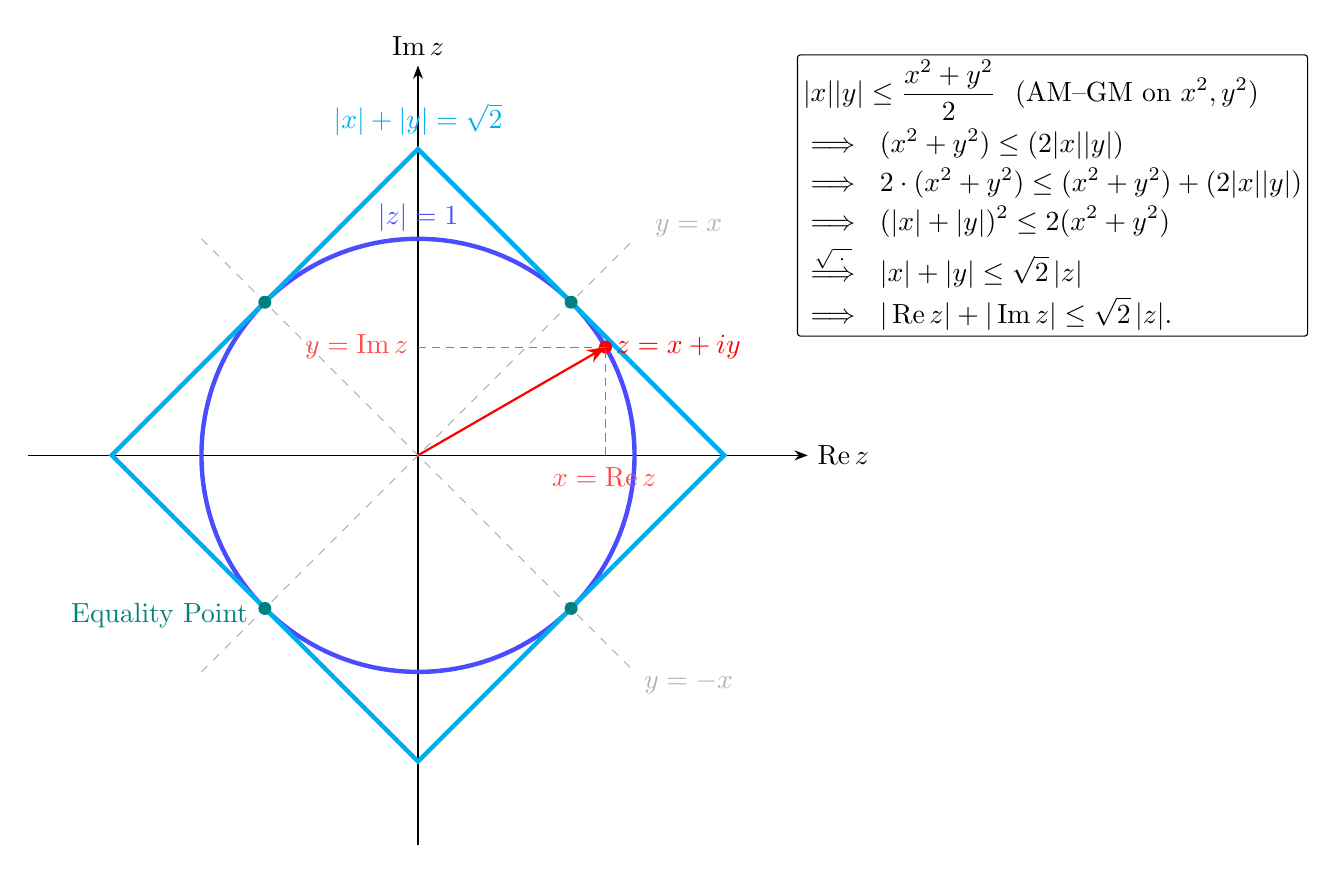
\begin{tikzpicture}[scale=2.75, >=Stealth]
	% axes
	\draw[->] (-1.8,0) -- (1.8,0) node[right] {$\Re z$};
	\draw[->] (0,-1.8) -- (0,1.8) node[above] {$\Im z$};
	
	% unit circle |z|=1
	\draw[ultra thick,blue!70] (0,0) circle (1);
%	\draw[ultra thick,blue!70, opacity=.5] (0,0) circle (0.7207);
	\node[blue!70] at (0,1.1) {$|z|=1$};
	
	% diamond |x|+|y|=sqrt(2)  (vertices at (±√2,0),(0,±√2))
	% use √2 ≈ 1.4142
	\draw[ultra thick,cyan] ( 1.4142,0) -- (0, 1.4142) -- (-1.4142,0) -- (0,-1.4142) -- cycle;
	\node[cyan] at (0,1.55) {$|x|+|y|=\sqrt{2}$};
	
	% equality rays y=±x
	\draw[dashed,gray!60] (-1,-1) -- (1,1);
	\draw[dashed,gray!60] (-1, 1) -- (1,-1);
	\node[gray!60] at (1.25,1.05) {$y=x$};
	\node[gray!60] at (1.25,-1.05) {$y=-x$};
	
	\foreach \X/\Y in {0.7071/0.7071, 0.7071/-0.7071, -0.7071/0.7071, -0.7071/-0.7071}{
		\fill[teal] (\X,\Y) circle (0.03);
	}
	\node[teal,anchor=east] at (-0.74,-0.74) {Equality Point
%		$\bigl(\tfrac{1}{\sqrt2},\tfrac{1}{\sqrt2}\bigr)$
	};
	
	% a sample point on the circle (theta = 30°)
	% coordinates: (cos 30°, sin 30°) ≈ (0.8660, 0.5)
	\fill[red] (0.8660,0.5000) circle (0.03);
	\draw[red,->,thick] (0,0) -- (0.8660,0.5000) node[right] {$z=x+iy$};
	
	% helper projections to visualize |x| and |y|
	\draw[red!70,densely dashed] (0.8660,0) -- (0.8660,0.5000);
	\draw[red!70,densely dashed] (0,0.5000) -- (0.8660,0.5000);
	\node[red!70] at (0.86,-0.10) {$x=\Re z$};
	\node[red!70, left] at (0,0.50) {$y=\Im z$};
	
	% AM-GM derivation (compact)
	\node[align=left,draw,rounded corners=1pt,inner sep=2pt,anchor=west] at (1.75,1.2)
	{$\displaystyle |x||y|\le\frac{x^2+y^2}{2}\ \ (\text{AM--GM on }x^2,y^2)$\\[2pt]
		$\displaystyle \implies\ (x^2+y^2)\le (2|x||y|)$\\[2pt]
		$\displaystyle \implies\ 2\cdot (x^2+y^2)\le(x^2+y^2)+(2|x||y|)$\\[2pt]
		$\displaystyle \implies\ (|x|+|y|)^2\le 2(x^2+y^2)$\\[2pt]
		$\displaystyle \overset{\sqrt{\;\cdot\;}}{\implies}\ |x|+|y|\le \sqrt{2}\,|z|$\\[2pt]
		$\displaystyle \implies\ |\Re z|+|\Im z|\le \sqrt{2}\,|z|.$};
\end{tikzpicture}
\end{center}
\end{proof}
\item By factoring $z^4-4z+3$ into two quadratic factors show that if $z$ lies on the circle $|z|=2$, then \[
\left|\frac{1}{z^4-4z^2+3}\right|\le \frac13.
\]
\begin{proof}[\Sol]
Since $z^4-4z^2+3 \;=\; (z^2-1)(z^2-3)$, we have \[
\left\lvert z^4-4z^2+3 \right\rvert
= \lvert z^2-1\rvert\,\lvert z^2-3\rvert.
\]
For $\lvert z\rvert=2$ one has $\lvert z^2\rvert=\lvert z\rvert^2=4$. By the triangle inequality,
\[
\lvert z^2-1\rvert \;\ge\; \bigl|\,\lvert z^2\rvert-\lvert 1\rvert\,\bigr| = \lvert 4-1\rvert = 3,
\qquad
\lvert z^2-3\rvert \;\ge\; \bigl|\,\lvert z^2\rvert-\lvert 3\rvert\,\bigr| = \lvert 4-3\rvert = 1.
\]
Hence
\[
\lvert z^4-4z^2+3\rvert \;\ge\; 3\cdot 1 \;=\; 3,
\]
and therefore
\[
\left\lvert\frac{1}{z^4-4z^2+3}\right\rvert \;=\; \frac{1}{\lvert z^4-4z^2+3\rvert} \;\le\; \frac{1}{3}.
\]

\begin{center}
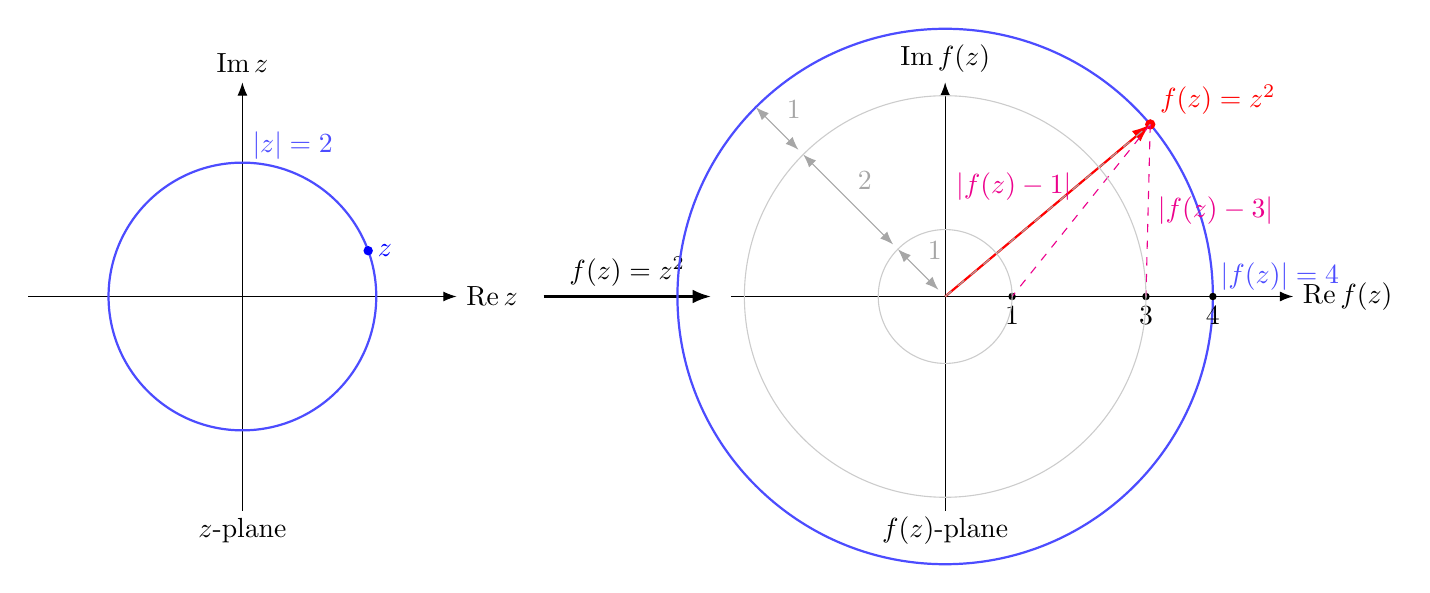
\begin{tikzpicture}[>=Latex,scale=.85]
	
	%================ z-plane =================
	\begin{scope}
		% axes
		\draw[->] (-3.2,0) -- (3.2,0) node[right] {$\Re z$};
		\draw[->] (0,-3.2) -- (0,3.2) node[above] {$\Im z$};
		\node at (0,-3.5) {$z$-plane};
		
		% circle |z|=2
		\draw[thick,blue!70] (0,0) circle (2);
		\node[blue!70] at (0.75,2.25) {$|z|=2$};
		
		% sample point z with |z|=2, angle ~20°
		% coordinates: 2*(cos20, sin20) ≈ (1.8794, 0.6840)
		\fill[blue] (1.8794,0.6840) circle (2pt)
		node[anchor=west] {$z$};
		
		% mapping arrow
		\draw[->,thick] (4.5,0) -- (7,0) node[midway,above] {$f(z)=z^2$};
	\end{scope}
	
	%================ w-plane =================
	\begin{scope}[xshift=10.5cm]
		% axes
		\draw[->] (-3.2,0) -- (5.2,0) node[right] {$\Re f(z)$};
		\draw[->] (0,-3.2) -- (0,3.2) node[above] {$\Im f(z)$};
		\node at (0,-3.5) {$f(z)$-plane};
		
		% circle |w|=4
		\draw[thick,blue!70] (0,0) circle (4);
		\node[blue!70] at (5,0.3) {$|f(z)|=4$};
		
		% two real points 1 and 3
		\fill (1,0) circle (1.6pt) node[below] {$1$};
		\fill (3,0) circle (1.6pt) node[below] {$3$};;
		\fill (4,0) circle (1.6pt) node[below] {$4$};
		
		% image point w = z^2 (angle doubles: ~40°), coords 4*(cos40, sin40) ≈ (3.0640, 2.5712)
		\fill[red] (3.0640,2.5712) circle (2.2pt) node[above right] {$f(z)=z^2$};
		\draw[red,->,thick] (0,0) -- (3.0640,2.5712);
		
		% distances |w-1| and |w-3|
		\draw[magenta, dashed] (3.0640,2.5712) -- (1,0) node[midway,above left] {$|f(z)-1|$};
		\draw[magenta, dashed] (3.0640,2.5712) -- (3,0) node[midway,right] {$|f(z)-3|$};
		
		% triangle-inequality lower bounds along the radial (origin->w) direction
		% show the radial segment length 4, and compare to 1 and 3
		\draw[dashed,gray!70] (0,0) -- (3.0640,2.5712); % radius 4
		% project the points 1 and 3 to the radial line via concentric circles
		\draw[gray!40] (0,0) circle (1);
		\draw[gray!40] (0,0) circle (3);
		
		% double-arrows indicating |4-1|=3 and |4-3|=1 on the radial line
		% place them near the ray with small offsets for clarity
		% marker for 0->1
		\draw[<->,gray!70] (-0.10,0.10) -- (-0.7071,0.7071)
		node[midway,above right] {$1$};
		% marker for 1->3
		\draw[<->,gray!70] (-0.7771,0.7771) -- (-2.1213,2.1213)
		node[midway,above right] {$2$};
		% marker for 3->4
		\draw[<->,gray!70] (-2.1913,2.1913) -- (-2.8284,2.8284)
		node[midway,above right] {$1$};
%		% marker for 0->4 (whole radius)
%		\node[gray!70] at (-1.9,1.2) {$|w|=4$};
		
%		% inequality reminders near the base points
%		\node[align=left,gray!60] at (0.9,1.3)
%		{$|w-1| \ge \bigl||w|-1\bigr|=3$};
%		\node[align=left,gray!60] at (2.6,-1.1)
%		{$|w-3| \ge \bigl||w|-3\bigr|=1$};
		
%		% product and reciprocal bounds
%		\node[draw,rounded corners=2pt,align=left,anchor=west] at (-3.0,-2.4)
%		{$\displaystyle |(w-1)(w-3)| \ge 3\cdot1=3$\\[4pt]
%			$\displaystyle \left|\frac{1}{(w-1)(w-3)}\right| \le \frac{1}{3}$};
	\end{scope}
	
\end{tikzpicture}
\end{center}

For equality in the reverse triangle inequalities we must have $z^2$ and the positive reals $1,3$ on the same ray from the origin, i.e.\ $z^2=4$. Together with $\lvert z\rvert=2$ this forces $z=\pm 2$, and indeed
\[
\lvert (\pm 2)^4 - 4(\pm 2)^2 + 3\rvert = \lvert 16-16+3\rvert = 3,
\]
so the bound is sharp precisely at $z=\pm 2$.
\end{proof}

\item Prove the finite geometric sum
\[
1+z+z^2+\cdots+z^n=\frac{1-z^{n+1}}{1-z}\quad(z\ne1)
\]
and deduce Lagrange's trigonometric identity
\[
1+\cos\theta+\cdots+\cos n\theta=\frac12+\frac{\sin\!\big((2n+1)\theta/2\big)}{2\sin(\theta/2)}\quad(0<\theta<2\pi).
\]
\newpage
\item Prove that the usual formula solves the quadratic equation \[
az^2+bz+c=0\quad (a\neq 0)
\] when the coefficient $a$,$b$, and $c$ are complex numbers. Specifically, by completing the square on the left-hand side, derive the \textbf{quadratic formula} \[
z=\frac{-b+\sqrt{b^2-4ac}}{2a},
\] where both square roots are to be considered when $b^2-4ac\neq 0$. Use this result to find the roots of the equation \[
z^2+2z+(1-i)=0.
\]
\begin{proof}[\Sol]
Since  \[
az^2+bz+c
= a\!\left(z^2+\frac{b}{a}z\right)+c
= a\!\left(z+\frac{b}{2a}\right)^{\!2}-a\!\left(\frac{b}{2a}\right)^{\!2}+c
= a\!\left(z+\frac{b}{2a}\right)^{\!2}-\frac{b^2}{4a}+c,
\] we have
\[
a\!\left(z+\frac{b}{2a}\right)^{\!2}=\frac{b^2}{4a}-c
\quad\Longleftrightarrow\quad
\left(z+\frac{b}{2a}\right)^{\!2}=\frac{b^2-4ac}{4a^2}.
\]
Taking square roots of both sides yields \[
z+\frac{b}{2a}=\pm\,\frac{\sqrt{\,b^2-4ac\,}}{2a},\quad\text{whence}\quad z=\frac{-b\pm\sqrt{\,b^2-4ac\,}}{2a}.
\] Consider $z^2+2z+(1-i)$ with \(a=1\), \(b=2\), and \(c=1-i\). The discriminant is \[
\Delta=b^2-4ac=4-4(1-i)=4i.
\] Since \[
\sqrt{i}=\frac{1+i}{\sqrt{2}}\quad\left(\text{indeed},\; \left(\frac{1+i}{\sqrt{2}}\right)^2=\frac{1+2i-1}{2}=i\right),
\] we may take $\sqrt{\Delta}=\sqrt{4i}=2\sqrt{i}= \sqrt{2}\,(1+i)$.
Therefore \[
z=\frac{-2\pm \sqrt{4i}}{2}
= -1 \pm \sqrt{i}
= -1 \pm \frac{1+i}{\sqrt{2}}.
\] Thus the roots are \[
z_1=-1+\frac{1+i}{\sqrt{2}},
\qquad
z_2=-1-\frac{1+i}{\sqrt{2}}.
\] Note that $z_1,z_2$ are roots of $(z+1)^2=i$.

\begin{center}
\begin{tikzpicture}[>=Latex, scale=4.0]
	% Axes
	\draw[->] (-2.2,0) -- (1.2,0) node[right] {$\Re z$};
	\draw[->] (0,-1.2) -- (0,1.2) node[above] {$\Im z$};
	% Center at -1 + 0i (from completing the square: (z+1)^2 = i)
	\fill (-1,0) circle (0.02) node[below] {$-1$};
	\draw[gray!60] (0,0) circle (1);
	\draw[blue,->, ultra thick] (0,0) -- (0.7071,0.7071)
	node[above right] {$\sqrt{i}=\dfrac{1+i}{\sqrt2}$};
	\filldraw[blue] (0.7071,0.7071) circle (.75pt);
	\node[blue] at (0.45,0.18) {$\arg=\tfrac{\pi}{4}$};
	\draw[cyan,->, ultra thick] (0,0) -- (0,1)
	node[left] {$i=(\sqrt{i})^2$};
	\filldraw[cyan] (0,1) circle (.75pt);
	\node[cyan] at (.2,0.8) {$\arg=\tfrac{\pi}{2}$};
	\draw[teal,->,ultra thick] (0,0) -- (-.7071,-.7071);
	% Roots as endpoints on the circle
	\fill[teal] (-.7071,-.7071) circle (0.03)
	node[below left] {$-\dfrac{1+i}{\sqrt2}$};
	\node[teal] at (-.45,-.18) {$\arg=-\tfrac{\pi}{4}$};
\begin{scope}[yshift=-2.75cm]
% Axes
\draw[->] (-2.2,0) -- (1.2,0) node[right] {$\Re z$};
\draw[->] (0,-1.2) -- (0,1.2) node[above] {$\Im z$};
% Center at -1 + 0i (from completing the square: (z+1)^2 = i)
\node[above, red] at (-1,.25) {$(z+1)^2 = i$};
\fill (-1,0) circle (0.02) node[below] {$-1$};
% Guide: circle of radius 1/sqrt(2) centered at -1
% 1/sqrt(2) ≈ 0.7071
%\draw[gray!60] (-1,0) circle (0.7071);
\draw[gray!60] (-1,0) circle (1);
\draw[gray!60] (0,0) circle (1);
%\node[gray!60] at (-0.35,0.12) {$r=\tfrac{1}{\sqrt2}$};
% Direction line for sqrt(i): 45 degrees through the center (-1,0)
\draw[dashed,gray!60] (-1-1.2,-1.2) -- (-1+1.2,1.2);
%\node[gray!60] at (-0.35,0.58) {$\arg=\tfrac{\pi}{4}$};
\node[blue] at (0.45,0.18) {$\arg=\tfrac{\pi}{4}$};
% The vector sqrt(i) drawn at the origin (reference)
\draw[blue,->,thick] (0,0) -- (0.7071,0.7071)
node[above right] {$\sqrt{i}=\dfrac{1+i}{\sqrt2}$};
%\node[blue] at (0.22,0.18) {$\tfrac{1}{\sqrt2}$};
% Same vector translated to start at -1 (to locate z1)
\draw[blue,->,thick] (-1,0) -- (-0.2929,0.7071);
% Opposite direction (to locate z2)
\draw[blue,->,thick] (-1,0) -- (-1.7071,-0.7071);
% Roots as endpoints on the circle
\fill[red] (-0.2929, 0.7071) circle (0.03)
node[above right] {$z_1=-1+\dfrac{1+i}{\sqrt2}$};
\fill[red] (-1.7071,-0.7071) circle (0.03)
node[below left] {$z_2=-1-\dfrac{1+i}{\sqrt2}$};
\end{scope}
\end{tikzpicture}
\end{center}

\end{proof}

\newpage
\item Determine the accumulation points of each sequence: \[
z_n=i^n,\quad, z_n=\frac{i^n}{n},\quad z_n=(-1)^n(1+i)\frac{n-1}{n}.
\]

\begin{proof}[\Sol]
	content...
\end{proof}
\item Prove that a finite set of points $z_1,z_2,\cdots, z_n$ cannot have any accumulation points.
\begin{proof}[\Sol]
Recall that $w\in\mathbb{C}$ is an accumulation point of $F$ iff for every $\varepsilon>0$ the punctured ball
$B(w,\varepsilon)\setminus\{w\}$ intersects $F$ (equivalently, $B(w,\varepsilon)$ contains a point of $F$ distinct from $w$).

Fix $w\in\mathbb{C}$. Consider the finite set of distances
\[
D:=\{\lvert w-z_k\rvert : 1\le k\le n\}\subset[0,\infty).
\]
Let $d:=\min D$. There are two cases.

\smallskip
\emph{Case 1: $w\notin F$.} Then $d>0$. For $\varepsilon:=\tfrac{d}{2}$ we have
$B(w,\varepsilon)\cap F=\varnothing$, hence $w$ is not an accumulation point.

\smallskip
\emph{Case 2: $w=z_j$ for some $j$.} If $n=1$, then $F=\{w\}$ and for any $\varepsilon>0$ small enough,
$B(w,\varepsilon)\cap(F\setminus\{w\})=\varnothing$, so $w$ is not an accumulation point. If $n\ge2$, put
\[
d':=\min_{k\neq j}\lvert z_j-z_k\rvert \;>\;0
\]
(since the minimum of finitely many positive numbers is positive). For $\varepsilon:=\tfrac{d'}{2}$ we have
$B(w,\varepsilon)\cap(F\setminus\{w\})=\varnothing$, so again $w$ is not an accumulation point.

\smallskip
Since \emph{no} $w\in\mathbb{C}$ can be an accumulation point of $F$, the set $F$ has no accumulation points.

\end{proof}
\end{enumerate}


\begin{definition}
	Let $(z_n)_{n\ge1}$ be a sequence in $\mathbb{C}$. A point $w\in\mathbb{C}$ is an \emph{accumulation point} (or \emph{subsequential limit}) of $(z_n)$ if there exists a strictly increasing map $k\mapsto n_k$ such that $\lim_{k\to\infty} z_{n_k}=w$.
\end{definition}

\begin{enumerate}
	\item[\textbf{(1)}] \(\displaystyle z_n=i^n.\)
	
	\emph{Claim.} The set of accumulation points is \(\{1,i,-1,-i\}\).
	
	\emph{Proof.} Since $i^n$ is $4$-periodic, the image set is $S:=\{1,i,-1,-i\}$, and each element of $S$ occurs infinitely many times. Hence for each $s\in S$ there exists the constant subsequence $z_{n_k}\equiv s$, so $s$ is an accumulation point. Conversely, any subsequence takes all its values in the finite set $S$, thus has a further constant subsequence by the pigeonhole principle; hence every accumulation point lies in $S$. Therefore the accumulation set equals $S$.
	
	\smallskip
	
	\item[\textbf{(2)}] \(\displaystyle z_n=\frac{i^n}{n}.\)
	
	\emph{Claim.} The only accumulation point is \(0\).
	
	\emph{Proof.} Since $\lvert i^n\rvert=1$ for all $n$, we have
	\[
	\lvert z_n\rvert=\frac{1}{n}\xrightarrow[n\to\infty]{}0.
	\]
	Thus $z_n\to 0$, and a convergent sequence has the singleton set $\{0\}$ as its accumulation set.
	
	\smallskip
	
	\item[\textbf{(3)}] \(\displaystyle z_n=(-1)^n(1+i)\,\frac{n-1}{n}.\)
	
	\emph{Claim.} The accumulation points are \(\{\,1+i,\,-(1+i)\,\}\).
	
	\emph{Proof.} Decompose into even/odd subsequences. For $n=2m$,
	\[
	z_{2m}=(1+i)\,\frac{2m-1}{2m}\xrightarrow[m\to\infty]{}1+i.
	\]
	For $n=2m+1$,
	\[
	z_{2m+1}=-(1+i)\,\frac{2m}{2m+1}\xrightarrow[m\to\infty]{}-(1+i).
	\]
	Hence $1+i$ and $-(1+i)$ are accumulation points. If $w$ is an accumulation point, then there exists $n_k\to\infty$ with $z_{n_k}\to w$. Since $\frac{n_k-1}{n_k}\to 1$ and $(-1)^{n_k}\in\{\pm1\}$, every limit $w$ must belong to $\{\pm(1+i)\}$. Thus the accumulation set is exactly $\{\,1+i,\,-(1+i)\,\}$.
\end{enumerate}

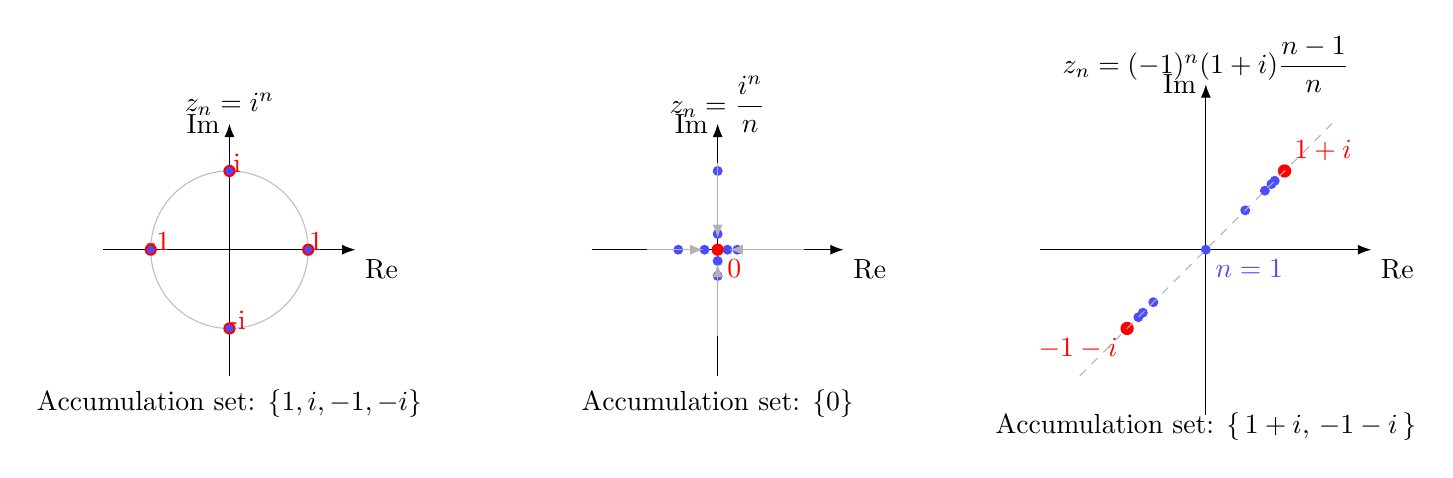
\begin{tikzpicture}[>=Latex,scale=1]
	
	% ================= Panel 1: z_n = i^n =================
	\begin{scope}
		% axes
		\draw[->] (-1.6,0) -- (1.6,0) node[below right] {$\Re$};
		\draw[->] (0,-1.6) -- (0,1.6) node[left] {$\Im$};
		\node at (0,1.85) {$z_n=i^n$};
		
		% unit circle (for context)
		\draw[gray!50] (0,0) circle (1);
		
		% the 4 accumulation points
		\foreach \X/\Y/\L in {1/0/{1}, 0/1/{i}, -1/0/{-1}, 0/-1/{-i}}{
			\fill[red] (\X,\Y) circle (2.2pt) node[shift={(0.1,0.1)}] {\L};
		}
		
		% a few terms n=0..7 to show cycling
		\foreach \P in {(1,0),(0,1),(-1,0),(0,-1),(1,0),(0,1),(-1,0),(0,-1)}{
			\fill[blue!70] \P circle (1.4pt);
		}
		
		\node[align=center] at (0,-1.95) {Accumulation set: $\{1,i,-1,-i\}$};
	\end{scope}
	
	% ================= Panel 2: z_n = i^n / n =================
	\begin{scope}[xshift=6.2cm]
		% axes
		\draw[->] (-1.6,0) -- (1.6,0) node[below right] {$\Re$};
		\draw[->] (0,-1.6) -- (0,1.6) node[left] {$\Im$};
		\node at (0,1.85) {$z_n=\dfrac{i^n}{n}$};
		
		% sample terms n=1..8:
		% (0,1),(-1/2,0),(0,-1/3),(1/4,0),(0,1/5),(-1/6,0),(0,-1/7),(1/8,0)
		\foreach \X/\Y in {0/1, -0.5/0, 0/-0.3333, 0.25/0, 0/0.2, -0.1667/0, 0/-0.1429, 0.125/0}{
			\fill[blue!70] (\X,\Y) circle (1.8pt);
		}
		
		% target 0
		\fill[red] (0,0) circle (2.2pt) node[below right] {$0$};
		
		% hint arrows
		\draw[->,gray!60] (0,1.1) -- (0,0.15);
		\draw[->,gray!60] (-0.9,0) -- (-0.18,0);
		\draw[->,gray!60] (0,-1.1) -- (0,-0.18);
		\draw[->,gray!60] (1.1,0) -- (0.15,0);
		
		\node[align=center] at (0,-1.95) {Accumulation set: $\{0\}$};
	\end{scope}
	
	% ================= Panel 3: z_n = (-1)^n(1+i)(n-1)/n =================
	\begin{scope}[xshift=12.4cm]
		% axes
		\draw[->] (-2.1,0) -- (2.1,0) node[below right] {$\Re$};
		\draw[->] (0,-2.1) -- (0,2.1) node[left] {$\Im$};
		\node at (0,2.35) {$z_n=(-1)^n(1+i)\dfrac{n-1}{n}$};
		
		% limit points at ±(1,1)
		\fill[red] (1,1) circle (2.4pt) node[above right] {$1+i$};
		\fill[red] (-1,-1) circle (2.4pt) node[below left] {$-1-i$};
		
		% terms n=1..8
		% n=1: 0
		\fill[blue!70] (0,0) circle (1.8pt) node[below right] {$n=1$};
		% n even:  (s,s),  s=(n-1)/n = 1-1/n
		% n odd:  (-s,-s)
		% n=2: s=1/2
		\fill[blue!70] (0.5,0.5) circle (1.8pt);
		% n=3: s=2/3
		\fill[blue!70] (-0.6667,-0.6667) circle (1.8pt);
		% n=4: s=3/4
		\fill[blue!70] (0.75,0.75) circle (1.8pt);
		% n=5: s=4/5
		\fill[blue!70] (-0.8,-0.8) circle (1.8pt);
		% n=6: s=5/6
		\fill[blue!70] (0.8333,0.8333) circle (1.8pt);
		% n=7: s=6/7
		\fill[blue!70] (-0.8571,-0.8571) circle (1.8pt);
		% n=8: s=7/8
		\fill[blue!70] (0.875,0.875) circle (1.8pt);
		
		% guide: dashed diagonal where the points lie
		\draw[dashed,gray!60] (-1.6,-1.6) -- (1.6,1.6);
		
		\node[align=center] at (0,-2.25) {Accumulation set: $\{\,1+i,\,-1-i\,\}$};
	\end{scope}
	
\end{tikzpicture}

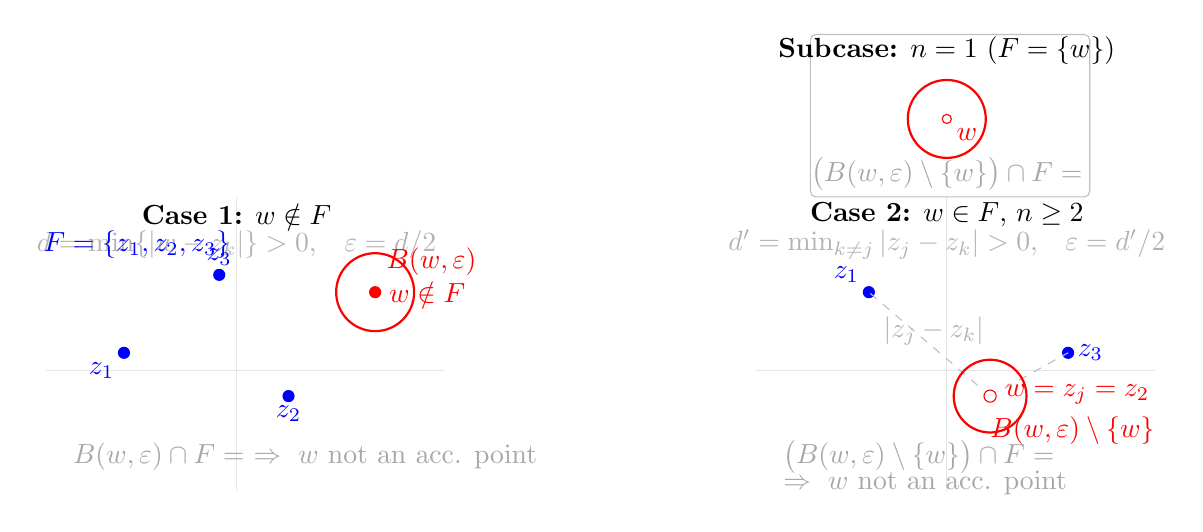
\begin{tikzpicture}[scale=1.1]
	
	% ================== Case 1: w not in F ==================
	\begin{scope}
		% axes (faint)
		\draw[gray!20] (-2.2,0) -- (2.4,0);
		\draw[gray!20] (0,-1.4) -- (0,2.0);
		
		\node[align=left] at (0,1.8) {\textbf{Case 1:} $w\notin F$};
		\node[align=left,gray!60] at (0,1.45) {$d=\min\{|w-z_k|\}>0$,\quad $\varepsilon=d/2$};
		
		% finite set F = {z1,z2,z3}
		\fill[blue] (-1.3,0.2) circle (2pt) node[below left] {$z_1$};
		\fill[blue] (0.6,-0.3)  circle (2pt) node[below] {$z_2$};
		\fill[blue] (-0.2,1.1)  circle (2pt) node[above] {$z_3$};
		\node[blue] at (-1.15,1.45) {$F=\{z_1,z_2,z_3\}$};
		
		% w not in F and its epsilon-ball
		\fill[red] (1.6,0.9) circle (2pt);
		\node[red,anchor=west] at (1.65,0.9) {$w\notin F$};
		
		% choose a ball around w that avoids F (epsilon = d/2 schematic)
		\draw[red,thick] (1.6,0.9) circle (0.45);
		\node[red] at (2.25,1.25) {$B(w,\varepsilon)$};
		
		% emphasize empty intersection
		\node[gray!70,anchor=west] at (-2.0,-1.0)
		{$B(w,\varepsilon)\cap F=\varnothing\ \Rightarrow\ \text{$w$ not an acc. point}$};
	\end{scope}
	
	% =============== Case 2: w in F, n >= 2 =================
	\begin{scope}[xshift=8.2cm]
		% axes (faint)
		\draw[gray!20] (-2.2,0) -- (2.4,0);
		\draw[gray!20] (0,-1.4) -- (0,2.0);
		
		\node[align=left] at (0,1.8) {\textbf{Case 2:} $w\in F$,\ $n\ge2$};
		\node[align=left,gray!60] at (0,1.45) {$d'=\min_{k\neq j}|z_j-z_k|>0$,\quad $\varepsilon=d'/2$};
		
		% finite set F = {z1=z_j, z2, z3}
		\fill[blue] (-0.9,0.9) circle (2pt) node[above left] {$z_1$};
		\fill[blue] (1.4,0.2)  circle (2pt) node[right] {$z_3$};
		
		% w = z2 (the point we're testing)
		\fill[red] (0.5,-0.3) circle (2pt);
		\node[red,anchor=west] at (0.56,-0.28) {$w=z_j=z_2$};
		
		% distances from w to neighbors (guides)
		\draw[gray!50,dashed] (0.5,-0.3) -- (-0.9,0.9);
		\draw[gray!50,dashed] (0.5,-0.3) -- (1.4,0.2);
		\node[gray!60] at (-0.15,0.45) {$|z_j-z_k|$};
		
		% punctured ball B(w, eps)\{w} with eps = d'/2 (schematic radius)
	\draw[red,thick] (0.5,-0.3) circle (0.42);
	% open/white dot to stress "punctured"
	\fill[white] (0.5,-0.3) circle (2.6pt);
	\draw[red] (0.5,-0.3) circle (2pt);
	\node[red] at (1.45,-0.7) {$B(w,\varepsilon)\setminus\{w\}$};
	
	% emphasize empty intersection with F\{w}
\node[gray!70,anchor=west] at (-2.0,-1.0)
{$\bigl(B(w,\varepsilon)\setminus\{w\}\bigr)\cap F=\varnothing$};
\node[gray!70,anchor=west] at (-2.0,-1.3)
{$\Rightarrow\ \text{$w$ not an acc. point}$};
\end{scope}

% =============== Inset: Case 2 with n=1 =================
\begin{scope}[xshift=8.2cm,yshift=2.9cm,scale=0.75]
% small box
\draw[gray!50,rounded corners=2pt] (-2.1,-1.2) rectangle (2.2,1.3);
\node at (0,1.05) {\textbf{Subcase:} $n=1$ ($F=\{w\}$)};

% w and its punctured ball
\fill[red] (0,0) circle (2pt) node[below right] {$w$};
\draw[red,thick] (0,0) circle (0.6);
\fill[white] (0,0) circle (2.6pt);
\draw[red] (0,0) circle (2pt);

\node[gray!70] at (0,-0.85)
{$\bigl(B(w,\varepsilon)\setminus\{w\}\bigr)\cap F=\varnothing$};
\end{scope}

\end{tikzpicture}


\newpage
\section{Analytic Functions}
\subsection{Functions of a Complex Variable}

\begin{definition}[Function and domain]
	Let $S\subset\C$. A \emph{function} $f$ on $S$ assigns to each $z\in S$ a complex number $w=f(z)$. The set $S$ is the \emph{domain} (domain of definition) of $f$. As real functions, we write $f(z)=u(x,y)+iv(x,y)$ for $z=x+iy$; in polar form, $f(z)=u(r,\theta)+iv(r,\theta)$. \end{definition}

\begin{definition}[Polynomials and rational functions]
	If $n\in\mathbb{Z}_{\ge0}$ and $a_0,\dots,a_n\in\C$ with $a_n\neq0$, the polynomial
	\[
	P(z)=a_0+a_1z+\cdots+a_n z^n
	\]
	has degree $n$. A \emph{rational function} is $P(z)/Q(z)$, defined where $Q(z)\neq0$.
\end{definition}

\begin{example}[Single-valued choice of a multiple-valued expression]
	For $z\neq0$ with $z=re^{i\theta}$ ($-\pi<\theta\le\pi$), the square root has two values $z^{1/2}=\pm\sqrt{r}\,e^{i\theta/2}$. Selecting the ``$+$'' value defines a single-valued branch on $\C^\times$; setting $f(0)=0$ extends it to $z=0$ (not analytic there). 
\end{example}

\subsection{Mappings}

\begin{definition}[Mapping, image, range, inverse image]
	Viewing $f$ as a mapping $f:S\to\C$, the \emph{image} of $z$ is $w=f(z)$; the image of $T\subset S$ is $f(T)$; the \emph{range} is $f(S)$. The \emph{inverse image} of $w_0$ is $\{z\in S:f(z)=w_0\}$.
\end{definition}

\begin{observation}[Basic geometric actions]
	\begin{itemize}[leftmargin=1.5em]
		\item $w=z+1$ translates one unit to the right.
		\item $w=iz=re^{i(\theta+\pi/2)}$ rotates by $\pi/2$ counterclockwise.
		\item $w=\bar z=x-iy$ reflects across the real axis.
	\end{itemize}
\end{observation}

\begin{example}[$w=z^2$ as a mapping]
	With $z=x+iy$, we have $w=u+iv$ where $u=x^2-y^2$, $v=2xy$. The first quadrant region $\{x\ge0,\,y\ge0,\,xy\le1\}$ maps onto the horizontal strip $\{0\le v\le2\}$.
\end{example}

\subsubsection*{Mapping by the exponential}
If $w=e^z=e^{x+iy}=e^x(\cos y+i\sin y)=\rho e^{i\theta}$, then $\rho=e^x$ and $\theta=y$. Thus vertical lines $\{x=\text{const}\}$ map to circles $\{|w|=\text{const}\}$ and horizontal lines $\{y=\text{const}\}$ map to rays $\{\arg w=\text{const}\}$.

\subsection{Limits and Related Theorems}

\begin{definition}[Limit]
	Let $f$ be defined on a deleted neighborhood of $z_0$. We say $\displaystyle\lim_{z\to z_0}f(z)=w_0$ if for each $\varepsilon>0$ there exists $\delta>0$ such that $|f(z)-w_0|<\varepsilon$ whenever $0<|z-z_0|<\delta$.
\end{definition}

\begin{theorem}[Uniqueness of limits]
	If the limit $\lim_{z\to z_0} f(z)$ exists, it is unique.\end{theorem}

\begin{example}
	For $f(z)=\tfrac{i}{2}z$ on $|z|<1$, $\lim_{z\to1}f(z)=\tfrac{i}{2}$. For $f(z)=\bar z/z$, $\lim_{z\to0}f(z)$ does \emph{not} exist: approaching along the real axis gives $1$, along the imaginary axis gives $-1$.
\end{example}

\begin{theorem}[Limit laws]
	If $\lim_{z\to z_0} f(z)=f_0$ and $\lim_{z\to z_0} g(z)=g_0$, then
	\[
	\lim_{z\to z_0}\big(f+g\big)=f_0+g_0,\quad
	\lim_{z\to z_0} f\,g=f_0g_0,\quad
	\lim_{z\to z_0}\frac{f}{g}=\frac{f_0}{g_0}\ (g_0\neq0).
	\]
	In particular, polynomials are continuous: $\lim_{z\to z_0}P(z)=P(z_0)$.
\end{theorem}

\subsubsection{Limits involving $\infty$}
Neighborhoods of $\infty$ are exteriors of large disks. One has
\[
\lim_{z\to z_0} f(z)=\infty \iff \lim_{z\to z_0}\frac{1}{f(z)}=0,\qquad
\lim_{z\to\infty} f(z)=w_0 \iff \lim_{z\to0} f\!\left(\tfrac1z\right)=w_0,
\]
and $\lim_{z\to\infty} f(z)=\infty \iff \lim_{z\to0} \frac{1}{f(1/z)}=0$.

\subsection{Continuity}

\begin{definition}[Continuity]
	$f$ is continuous at $z_0$ if $\lim_{z\to z_0}f(z)=f(z_0)$. It is continuous on a region $R$ if continuous at each $z_0\in R$.
\end{definition}

\begin{theorem}[Basic properties]
	Composition of continuous functions is continuous. If $f$ is continuous and $f(z_0)\neq0$, then $f$ is nonzero on some neighborhood of $z_0$. If $f=u+iv$, then $f$ is continuous at $z_0$ iff $u$ and $v$ are continuous there. If $R$ is closed and bounded and $f$ continuous on $R$, then $|f|$ attains a maximum on $R$ (boundedness).
\end{theorem}

\subsection{Derivatives}

\begin{definition}[Complex derivative]
	If $f$ is defined on a neighborhood of $z_0$, the derivative at $z_0$ is
	\[
	f'(z_0)=\lim_{z\to z_0}\frac{f(z)-f(z_0)}{z-z_0}
	=\lim_{\Delta z\to0}\frac{\Delta w}{\Delta z},\quad \Delta w=f(z_0+\Delta z)-f(z_0),
	\]
	when the limit exists.
\end{definition}

\begin{theorem}[Consequences]
	If $f'(z_0)$ exists then $f$ is continuous at $z_0$. Moreover,
	\[
	\frac{d}{dz}c=0,\qquad \frac{d}{dz}z=1,\qquad \frac{d}{dz}[c f]=c f',\qquad
	\frac{d}{dz}z^n=n z^{n-1}\ (n\in\mathbb{Z},\ z\neq0\text{ if }n<0),
	\]
	and the sum/product/quotient rules and chain rule hold exactly as in calculus.
\end{theorem}

\begin{example}
	$f(z)=z^2\Rightarrow f'(z)=2z$. The function $f(z)=\bar z$ has no complex derivative anywhere. The function $f(z)=|z|^2$ has derivative only at $z=0$ (value $0$).
\end{example}

\subsection{Cauchy--Riemann Equations}

Let $f=u+iv$ with $u,v$ real-valued.

\begin{theorem}[Cauchy--Riemann (CR) equations]
	If $f'(z_0)$ exists then the first partials of $u,v$ exist at $(x_0,y_0)$ and satisfy
	\[
	u_x(x_0,y_0)=v_y(x_0,y_0),\qquad u_y(x_0,y_0)=-v_x(x_0,y_0),
	\]
	and $f'(z_0)=u_x(x_0,y_0)+i\,v_x(x_0,y_0)$.
\end{theorem}

\begin{theorem}[Sufficient conditions]
	If $u_x,u_y,v_x,v_y$ exist in a neighborhood of $z_0$, are continuous at $z_0$, and satisfy the CR equations at $z_0$, then $f'(z_0)$ exists and equals $u_x+i v_x$.
\end{theorem}

\begin{example}
	$f(z)=z^2=x^2-y^2+i\,2xy$ satisfies CR everywhere and $f'(z)=2z$. For $f(z)=|z|^2=x^2+y^2$, the CR equations force $(x,y)=(0,0)$; hence $f'$ exists only at $0$. For $f(z)=e^z=e^x(\cos y+i\sin y)$ we have $f'(z)=e^z$ for all $z$.
\end{example}

\subsubsection*{CR equations in polar coordinates}
If $f=u(r,\theta)+iv(r,\theta)$ near $z_0=r_0e^{i\theta_0}\neq0$, the polar CR system is
\[
u_r=\frac1r v_\theta,\qquad v_r=-\frac1r u_\theta,
\]
and $f'(z_0)=e^{-i\theta_0}\big(u_r(r_0,\theta_0)+i\,v_r(r_0,\theta_0)\big)$.

\subsection{Analytic Functions}

\begin{definition}[Analytic/entire/singularity]
	$f$ is \emph{analytic} at $z_0$ if it has a derivative at every point of some neighborhood of $z_0$. If analytic at every point of $\C$, $f$ is \emph{entire}. If $f$ fails to be analytic at $z_0$ but is analytic arbitrarily close to $z_0$, then $z_0$ is a \emph{singular point} (singularity) of $f$.
\end{definition}

\begin{theorem}[Algebra and composition]
	Sums and products of analytic functions are analytic; a quotient $f/g$ is analytic where $g\neq0$. If $f$ is analytic in $D$ and $g$ is analytic on $f(D)$, then $g\circ f$ is analytic in $D$ with $(g\circ f)'=(g'\circ f)\,f'$.
\end{theorem}

\begin{theorem}[Zero derivative]
	If $f'(z)=0$ for all $z$ in a domain $D$, then $f$ is constant on $D$.
\end{theorem}

\begin{example}
	\[
	f(z)=\frac{z^3+4}{(z^2-3)(z^2+1)}
	\]
	is analytic on $\C\setminus\{\pm\sqrt{3},\,\pm i\}$. Also $f(z)=\cosh x\cos y+i\sinh x\sin y$ is entire since CR holds everywhere.
\end{example}

\begin{theorem}[Conjugate tests]
	If $f$ and $\bar f$ are both analytic in $D$, then $f$ is constant in $D$. If $f$ is analytic in $D$ and $|f|$ is constant, then $f$ is constant.
\end{theorem}

\subsection{Harmonic Functions}

\begin{definition}[Harmonicity]
	A real function $h(x,y)$ is \emph{harmonic} on a domain if it has continuous second partials and satisfies Laplace's equation
	\[
	\Delta h=h_{xx}+h_{yy}=0.
	\]
\end{definition}

\begin{theorem}[Harmonic components]
	If $f=u+iv$ is analytic in $D$, then $u$ and $v$ are harmonic in $D$. Conversely, if $u$ and $v$ are harmonic and satisfy the CR equations in $D$, then $f=u+iv$ is analytic in $D$; $v$ is then a \emph{harmonic conjugate} of $u$.
\end{theorem}

\begin{example}
	$f(z)=\dfrac{i}{z^2}$ is analytic on $\C\setminus\{0\}$; writing it as
	\[
	\frac{i}{z^2}=\frac{2xy+i(x^2-y^2)}{(x^2+y^2)^2}=u+iv,
	\]
	both $u$ and $v$ are harmonic away from the origin. For $u(x,y)=y^3-3x^2y$, a harmonic conjugate is $v(x,y)=-3xy^2+x^3+C$.
\end{example}

\subsubsection*{Uniqueness and reflection}
\begin{lemma}[Identity lemma]
	If $f$ is analytic in $D$ and vanishes on a set with a limit point in $D$ (e.g.\ a subdomain or line segment), then $f\equiv0$ in $D$.
\end{lemma}

\begin{theorem}[Uniqueness from values]
	An analytic function in $D$ is uniquely determined in $D$ by its values on any subdomain or line segment contained in $D$.
\end{theorem}

\begin{theorem}[Reflection principle (real axis)]
	Let $D$ contain a symmetric neighborhood of a real segment. Then $f(\bar z)=\overline{f(z)}$ in $D$ iff $f(x)\in\R$ for all $x$ on that segment.
\end{theorem}
\newpage
\section*{Exercises}
\begin{enumerate}[\bfseries 1.]
\item Show that the following limit does not exitst \[
\lim_{z\to0}\Big(\frac{\bar z}{z}\Big)^2
\] Do this by letting nonzero points $z=(x,0)$ and $z=(x,x)$ approach the origin. (Note that it is not sufficient to simply consider points $z=(x,0)$ and $z=(0,y)$.)
\begin{proof}[\Sol]
Let $z=x+iy\in\C$ with $x,y\in\mathbb{R}$. Then \[
\left(\frac{\overline{z}}{z}\right)^{\!2}
=\left(\frac{x-iy}{x+iy}\right)^{\!2}.
\] If $z=re^{i\theta}$ with $r>0$, then $\bar z/z=e^{-2i\theta}$, so $|(\bar z/z)^2|=|e^{-4i\theta}|=1$.
\begin{center}
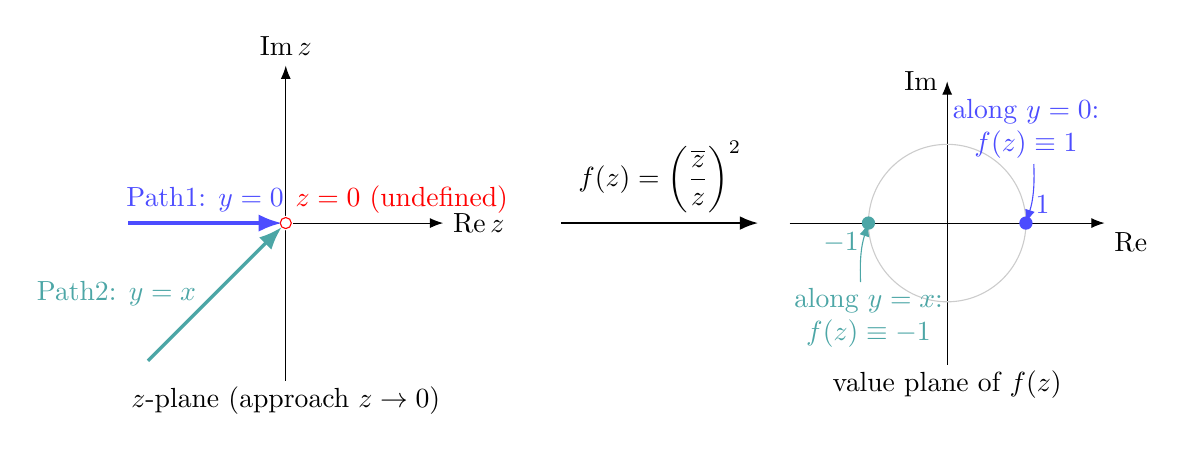
\begin{tikzpicture}[>=Latex,scale=1]
% =============== z-plane (paths to the origin) ===============
\begin{scope}
	% axes
	\draw[->] (-2.0,0) -- (2.0,0) node[right] {$\Re z$};
	\draw[->] (0,-2.0) -- (0,2.0) node[above] {$\Im z$};
	\node at (0,-2.25) {$z$-plane (approach $z\to 0$)};
	
	% origin as a hole (z=0 excluded)
	\fill[white] (0,0) circle (2.6pt);
	\draw[red] (0,0) circle (2pt) node[above right] {$z=0$ (undefined)};
	
	% Path 1: real axis y=0 (blue)
	\draw[blue!70,very thick,->] (-2,0) -- (-0.05,0) node[midway, above] {Path1: $y=0$};
	
	% Path 2: diagonal y=x (teal)
	\draw[teal!70,very thick,->] (-1.75,-1.75) -- (-0.05,-0.05) node[midway, xshift=-1.25cm] {Path2: $y=x$};
\end{scope}
% =============== mapping arrow ===============
\draw[->,thick] (3.5,0) -- (6,0)
node[midway,above] {$f(z)=\left(\dfrac{\overline z}{z}\right)^2$};
% =============== value plane (outputs) ===============
\begin{scope}[xshift=8.4cm]
	% axes
	\draw[->] (-2,0) -- (2,0) node[below right] {$\Re$};
	\draw[->] (0,-1.8) -- (0,1.8) node[left] {$\Im$};
	\node at (0,-2.05) {value plane of $f(z)$};
	
	% unit circle (context): |(\bar z/z)^2| = 1 for z≠0
	\draw[gray!40] (0,0) circle (1);
	
	% images of the two paths (constants 1 and -1)
	% Path 1 (y=0) -> 1
	\fill[blue!70] (1,0) circle (2.4pt) node[above right] {$1$};
	\draw[blue!70,->] (1.1,.75) to[bend left=10] (1,0);
	\node[blue!70,align=center] at (1,1.2)
	{along $y=0$:\\ $f(z)\equiv 1$};
	
	% Path 2 (y=x) -> -1
	\fill[teal!70] (-1,0) circle (2.4pt) node[below left] {$-1$};
	\draw[teal!70,->] (-1.1,-0.75) to[bend left=10] (-1,0);
	\node[teal!70,align=center] at (-1,-1.2)
	{along $y=x$:\\ $f(z)\equiv -1$};
	
%	% conclusion box
%	\node[draw,rounded corners=2pt,align=left,anchor=north] at (0,-1.25)
%	{$\displaystyle \lim_{z\to 0}\left(\frac{\overline z}{z}\right)^2\ \text{does not exist},$\\
%		since the limits along $y=0$ and $y=x$ differ.};
\end{scope}
\end{tikzpicture}
\end{center}
\medskip
\noindent\textbf{(1) Path 1: approach along the real axis $y=0$}

Let $z=x+0i=x$ with $x\in\mathbb{R}\setminus\{0\}$ and $x\to 0$. Then $
\displaystyle\left(\frac{\overline{z}}{z}\right)^2
=\left(\frac{x}{x}\right)^2
=1$.

\medskip
\noindent\textbf{(2) Path 2: approach along the diagonal $y=x$}

Let $z=x+ix=(1+i)x$ with $x\in\mathbb{R}\setminus\{0\}$ and $x\to 0$. Then
\[
\frac{\overline{z}}{z}
=\frac{\overline{(1+i)x}}{(1+i)x}
=\frac{(1-i)\,x}{(1+i)\,x}
=\frac{1-i}{1+i}
=\frac{(1-i)^2}{(1+i)(1-i)}
=\frac{1-2i+i^2}{1- i^2}
=\frac{1-2i-1}{2}
=\frac{-2i}{2}
=-i.
\]
Hence
\[
\left(\frac{\overline{z}}{z}\right)^2
=(-i)^2
=-1.
\] 

\medskip
\noindent\textbf{(3) Conclusion}

Since the limits along these two paths are different (namely $1$ and $-1$), the limit cannot exist.
\end{proof}
%	\item[X] Compute $\displaystyle \lim_{z\to\infty}\frac{4z^2}{(z-1)^2}$, $\ \lim_{z\to1}\frac{1}{(z-1)^3}$, and $\ \lim_{z\to\infty}\frac{z^2+1}{z-1}$.
%	\item[X] Suppose $f(z_0)=g(z_0)=0$ with $g'(z_0)\neq0$ and both derivatives exist. Prove
%	\[
%	\lim_{z\to z_0}\frac{f(z)}{g(z)}=\frac{f'(z_0)}{g'(z_0)}.
%	\]
\item Let \[
f(z)=\begin{cases} \bar z^2/z,& z\neq0,\\ 0,& z=0.\end{cases}
\] Show that if $z=0$, then $\Delta w/\Delta z=1$ at eatch nonzero point on the real and imaginary axes in the $\Delta z$, or $\Delta x\Delta y$, plane. Then show that $\Delta w/\Delta z=-1$ at each nonzero point $(\Delta x, \Delta y)$ on the line $\Delta y=\Delta x$ in that plane. Conclude from these observations that $f'(0)$ does not exist. Note that to obtain this result, it is not sufficient to consider only horizontal and vertical approaches to the origin in the $\Delta z$ plane.
\begin{proof}
Let $\frac{\Delta w}{\Delta z}
=\frac{f(\Delta z)-f(0)}{\Delta z}
\quad(\Delta z\neq 0)$. Since $f(0)=0$, for $\Delta z\neq0$, $\displaystyle
\frac{\Delta w}{\Delta z}
=\frac{f(\Delta z)}{\Delta z}
=\frac{\overline{\Delta z}^{\,2}}{(\Delta z)^2}$.

\medskip
\noindent\textbf{(1) Real and imaginary axes.}
\begin{itemize}
	\item Real axis: $\Delta z=x$ with $x\in\mathbb{R}\setminus\{0\}$, $\displaystyle
	\frac{\Delta w}{\Delta z}=\frac{\overline{x}^{\,2}}{x^2}=\frac{x^2}{x^2}=1$.
	\begin{center}
	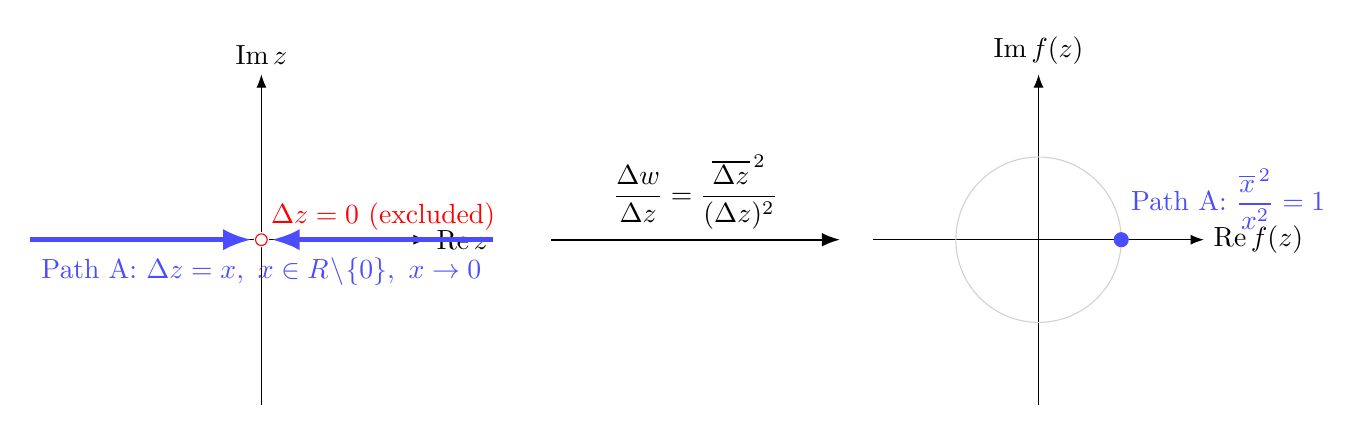
\begin{tikzpicture}[>=Latex,scale=1.05]	
		%================ z-plane: explicit paths =================
		\begin{scope}
			% axes
			\draw[->] (-2,0) -- (2,0) node[right] {$\Re z$};
			\draw[->] (0,-2) -- (0,2) node[above] {$\Im z$};
			% hole at the origin (Delta z = 0 excluded)
			\fill[white] (0,0) circle (2.6pt);
			\draw[red] (0,0) circle (2pt) node[above right] {$\Delta z=0$ (excluded)};
			% Path A: real axis, Δz = x, x→0, x≠0
			\draw[line width=1.6pt,blue!70,->] (-2.8,0) -- (-0.12,0);
			\draw[line width=1.6pt,blue!70,->] ( 2.8,0) -- ( 0.12,0);
			\node[blue!70,anchor=north] at (0,-0.10)
			{$\displaystyle \text{Path A: }\Delta z=x,\ x\in\mathbb R\!\setminus\!\{0\},\ x\to 0$};
		\end{scope}
		%================ mapping arrow =================
		\draw[->,thick] (3.5,0) -- (7,0)
		node[midway,above] {$\displaystyle \frac{\Delta w}{\Delta z}=\frac{\overline{\Delta z}^{\,2}}{(\Delta z)^2}$};
		%================ value plane: constant images =================
		\begin{scope}[xshift=9.4cm]
			% axes
			\draw[->] (-2,0) -- (2,0) node[right] {$\Re f(z)$};
			\draw[->] (0,-2) -- (0,2) node[above] {$\Im f(z)$};
			%	\node at (0,-2.55) {$f(z)$-plane of $\Delta w/\Delta z$};
			% unit circle for context (|Δw/Δz|=1 for Δz≠0)
			\draw[gray!35] (0,0) circle (1);
			% Image of Path A (real axis): constant 1
			\fill[blue!70] (1,0) circle (2.6pt) node[above right] {$\displaystyle \text{Path A: } \frac{\overline{x}^{\,2}}{x^2}=1$};
		\end{scope}
	\end{tikzpicture}
	\end{center}
	\item Imaginary axis: $\Delta z=iy$ with $y\in\mathbb{R}\setminus\{0\}$, $\displaystyle
	\frac{\Delta w}{\Delta z}
	=\frac{\overline{iy}^{\,2}}{(iy)^2}
	=\frac{(-iy)^2}{(iy)^2}
	=\frac{-y^2}{-y^2}=1$.
	\begin{center}
	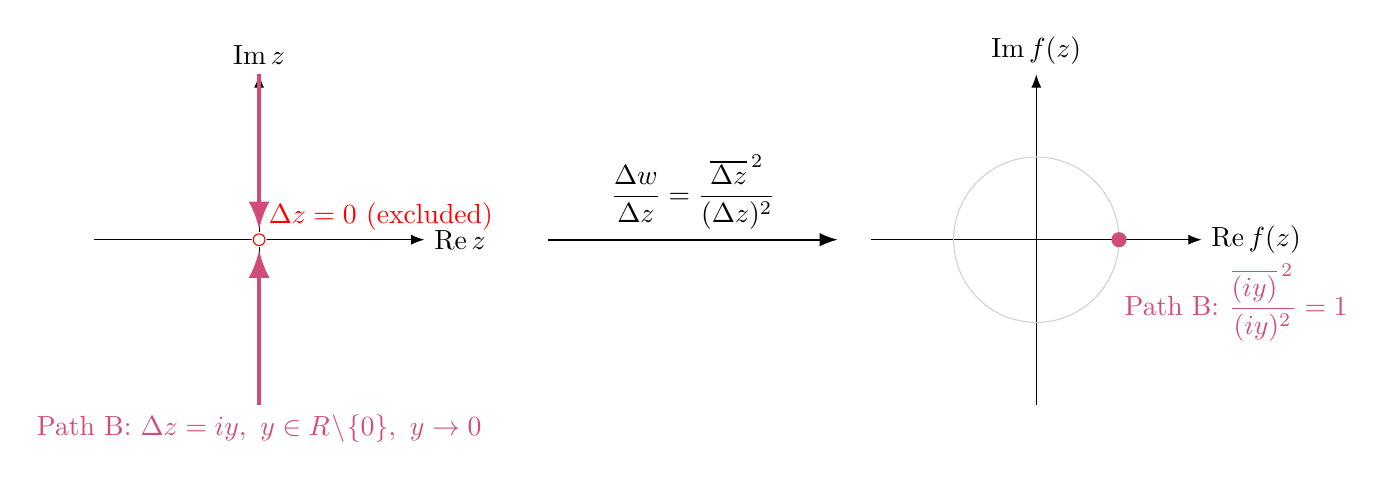
\begin{tikzpicture}[>=Latex,scale=1.05]	
		%================ z-plane: explicit paths =================
		\begin{scope}
			% axes
			\draw[->] (-2,0) -- (2,0) node[right] {$\Re z$};
			\draw[->] (0,-2) -- (0,2) node[above] {$\Im z$};
			% hole at the origin (Delta z = 0 excluded)
			\fill[white] (0,0) circle (2.6pt);
			\draw[red] (0,0) circle (2pt) node[above right] {$\Delta z=0$ (excluded)};
			% Path B: imaginary axis, Δz = iy, y→0, y≠0
			\draw[line width=1.6pt,purple!70,->] (0,-2.0) -- (0,-0.12);
			\draw[line width=1.6pt,purple!70,->] (0, 2.0) -- (0, 0.12);
			\node[purple!70,anchor=north] at (0,-2)
			{$\displaystyle \text{Path B: }\Delta z=iy,\ y\in\mathbb R\!\setminus\!\{0\},\ y\to 0$};
		\end{scope}
		%================ mapping arrow =================
		\draw[->,thick] (3.5,0) -- (7,0)
		node[midway,above] {$\displaystyle \frac{\Delta w}{\Delta z}=\frac{\overline{\Delta z}^{\,2}}{(\Delta z)^2}$};
		%================ value plane: constant images =================
		\begin{scope}[xshift=9.4cm]
			% axes
			\draw[->] (-2,0) -- (2,0) node[right] {$\Re f(z)$};
			\draw[->] (0,-2) -- (0,2) node[above] {$\Im f(z)$};
			%	\node at (0,-2.55) {$f(z)$-plane of $\Delta w/\Delta z$};
			% unit circle for context (|Δw/Δz|=1 for Δz≠0)
			\draw[gray!35] (0,0) circle (1);
			% Image of Path B (imag axis): constant 1
			\fill[purple!70] (1,0) circle (2.6pt);
			\node[purple!70,anchor=north west] at (0.95,-0.18)
			{$\displaystyle \text{Path B: } \frac{\overline{(iy)}^{\,2}}{(iy)^2}=1$};
		\end{scope}
	\end{tikzpicture}
	\end{center}
\end{itemize}

\noindent\textbf{(2) Line $\Delta y=\Delta x$.}
Let $\Delta z=(1+i)x$ with $x\in\mathbb{R}\setminus\{0\}$. Then
\[
\frac{\Delta w}{\Delta z}
=\frac{\overline{(1+i)x}^{\,2}}{((1+i)x)^2}
=\frac{((1-i)x)^2}{((1+i)x)^2}
=\frac{(1-i)^2}{(1+i)^2}
=\frac{-2i}{2i}=-1.
\]
\begin{center}
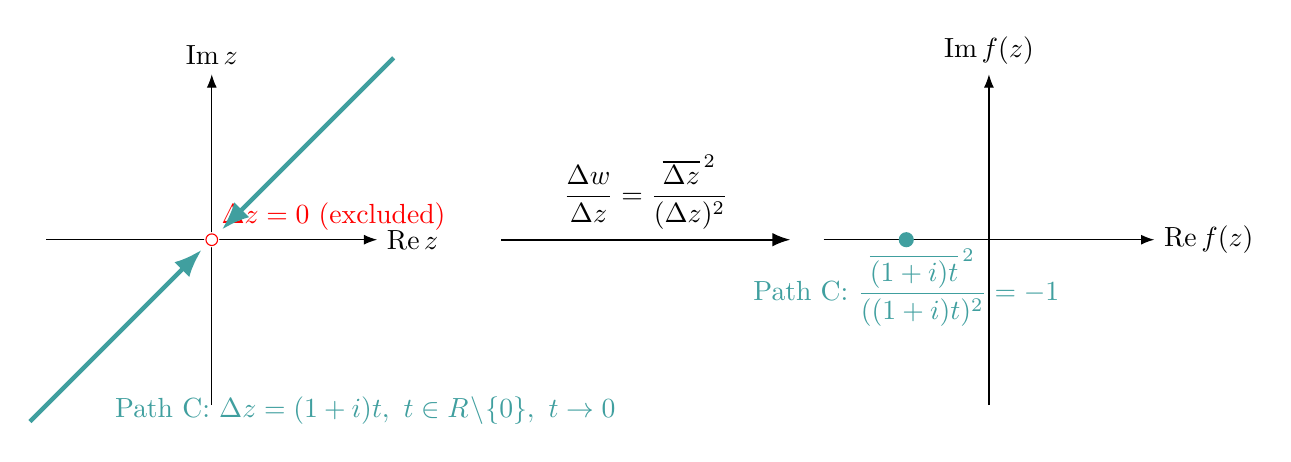
\begin{tikzpicture}[>=Latex,scale=1.05]	
%================ z-plane: explicit paths =================
\begin{scope}
	% axes
	\draw[->] (-2,0) -- (2,0) node[right] {$\Re z$};
	\draw[->] (0,-2) -- (0,2) node[above] {$\Im z$};
	%	\node at (0,-2.55) {$z$-plane (approach $\Delta z\to 0$)$\,$};	
	% hole at the origin (Delta z = 0 excluded)
	\fill[white] (0,0) circle (2.6pt);
	\draw[red] (0,0) circle (2pt) node[above right] {$\Delta z=0$ (excluded)};
	% Path C: diagonal Δy=Δx, i.e., Δz = (1+i)t, t→0, t≠0
	\draw[line width=1.6pt,teal!75,->] (-2.2,-2.2) -- (-0.12,-0.12);
	\draw[line width=1.6pt,teal!75,->] ( 2.2, 2.2) -- ( 0.12, 0.12);
	\node[teal!75,anchor=south east] at (5,-2.35)
	{$\displaystyle \text{Path C: }\Delta z=(1+i)t,\ t\in\mathbb R\!\setminus\!\{0\},\ t\to 0$};
\end{scope}
%================ mapping arrow =================
\draw[->,thick] (3.5,0) -- (7,0)
node[midway,above] {$\displaystyle 
	\frac{\Delta w}{\Delta z}=\frac{\overline{\Delta z}^{\,2}}{(\Delta z)^2}
	%	\displaystyle \,f(z)=\begin{cases}
		%		\overline z^{\,2}/z &\text{if}\; z\neq 0\\
		%		0 &\text{if}\; z=0
		%	\end{cases}
	$};
%================ value plane: constant images =================
\begin{scope}[xshift=9.4cm]
	% axes
	\draw[->] (-2,0) -- (2,0) node[right] {$\Re f(z)$};
	\draw[->] (0,-2) -- (0,2) node[above] {$\Im f(z)$};
	%	\node at (0,-2.55) {$f(z)$-plane of $\Delta w/\Delta z$};
	% Image of Path C (diagonal): constant -1
	\fill[teal!75] (-1,0) circle (2.6pt) node[below] {$\displaystyle \text{Path C: } \frac{\overline{(1+i)t}^{\,2}}{((1+i)t)^2}=-1$};
\end{scope}
\end{tikzpicture}
\end{center}
\medskip
\noindent\textbf{(3) Conclusion.}
Since the difference quotient equals $1$ along the axes but $-1$ along the line $\Delta y=\Delta x$, the limit
\[
\lim_{\Delta z\to 0}\frac{f(\Delta z)-f(0)}{\Delta z}
\]
depends on the path and therefore does not exist. Consequently, $f'(0)$ does not exist.
\end{proof}	
\newpage
\item Let \[
f(z)=\bar z,\quad f(z)=2x+ixy^2,\quad f(z)=e^{\bar z}
\] Then show that $f'(z)$ does not exists at any point.
\begin{proof}[\Sol]
Let \(z=x+iy\) and \(f(z)=u+iv\) with $x,y,u,v\in\R$. The Cauchy--Riemann equations \[
u_x=v_y,\qquad u_y=-\,v_x
\]
are necessary and sufficient for complex differentiability.

\medskip
\noindent\textbf{(1) \(f_1(z)=\overline z=\overline{x+iy}=x-iy\).}

Here \(u(x,y)=x,\ v(x,y)=-y\). Thus \[
u_x=1,\quad u_y=0,\quad v_x=0,\quad v_y=-1.
\]
The CR require \(u_x=v_y\), i.e.\ \(1=-1\), which is impossible. Hence \(f_1'\) does not exist anywhere.

\medskip
\noindent\textbf{(2) \(f_2(z)=2x+i\,x y^{2}\).}

Here \(u(x,y)=2x,\ v(x,y)=x y^{2}\). Thus
\[
u_x=2,\quad u_y=0,\quad v_x=y^{2},\quad v_y=2xy.
\]
The CR demand \[
\begin{cases} u_x=v_y\\ u_y=-v_x \end{cases}\implies
\begin{cases} 2=2xy\\ 0=y^2 \end{cases}\implies
\begin{cases} xy=1\\ y=0 \end{cases}.
\] These cannot hold simultaneously for any \(x\). Hence CR fail at every point, so \(f_2'\) exists nowhere.

\medskip
\noindent\textbf{(3) \(f_3(z)=e^{\overline z}\).}

Let \(\overline z=x-iy\). Then $f_3(x,y)=e^{x-iy}=e^{x}(\cos y-i\sin y)$, so \[
u(x,y)=e^{x}\cos y,\qquad v(x,y)=-\,e^{x}\sin y.
\] Compute \[
u_x=e^{x}\cos y,\quad u_y=-e^{x}\sin y,\quad
v_x=-e^{x}\sin y,\quad v_y=-e^{x}\cos y.
\] The CR give \[
\begin{cases} u_x=v_y\\ u_y=-v_x \end{cases}\implies
\begin{cases} e^x\cos y=-e^x\cos y\\ -e^x\sin y=+e^x\sin y \end{cases}\implies
\begin{cases} \cos y = 0\\ \sin y=0 \end{cases}.
\] These cannot hold simultaneously for any \(y\). Hence CR fail everywhere and \(f_3'\) exists nowhere.
\end{proof}
\item Let $f(z)=u(x,y)+i v(x,y)$ be given by \[
f(z)=\begin{cases}
	\bar z^2/z &: z\neq 0 \\
	0 &: z=0.
\end{cases}
\] Verify that the Cauchy--Riemann equations $u_x=v_y$ and $u_y=-v_x$ are satisfied at the origin $z=(0,0)$.
\begin{proof}
Write $z=x+iy$ and define
\[
f(z)=
\begin{cases}
	\dfrac{\overline z^{\,2}}{z}, & (x,y)\neq(0,0),\\[4pt]
	0, & (x,y)=(0,0).
\end{cases}
\]
Let $f=u+iv$. We compute the first-order partials of $u,v$ at $(0,0)$ by restricting to the
coordinate axes.

\medskip
\noindent\textbf{Along the $x$-axis ($y=0$):} For $x\neq0$,
\[
f(x,0)=\frac{\overline{x}^{\,2}}{x}=x,
\]
hence $u(x,0)=x$ and $v(x,0)=0$. Therefore
\[
u_x(0,0)=\lim_{h\to0}\frac{u(h,0)-u(0,0)}{h}
=\lim_{h\to0}\frac{h-0}{h}=1,
\quad
v_x(0,0)=\lim_{h\to0}\frac{v(h,0)-v(0,0)}{h}
=\lim_{h\to0}\frac{0-0}{h}=0.
\]

\medskip
\noindent\textbf{Along the $y$-axis ($x=0$):} For $y\neq0$,
\[
f(0,y)=\frac{\overline{iy}^{\,2}}{iy}=\frac{(-iy)^2}{iy}=\frac{-y^2}{iy}=iy,
\]
so $u(0,y)=0$ and $v(0,y)=y$. Hence
\[
u_y(0,0)=\lim_{k\to0}\frac{u(0,k)-u(0,0)}{k}
=\lim_{k\to0}\frac{0-0}{k}=0,
\quad
v_y(0,0)=\lim_{k\to0}\frac{v(0,k)-v(0,0)}{k}
=\lim_{k\to0}\frac{k-0}{k}=1.
\]

\medskip
Thus at $(0,0)$ we have
\[
u_x(0,0)=1,\qquad v_y(0,0)=1,\qquad u_y(0,0)=0,\qquad v_x(0,0)=0,
\]
and consequently the Cauchy--Riemann equations
\(
u_x=v_y
\)
and
\(
u_y=-v_x
\)
hold at the origin.

\begin{remark}
	Although the Cauchy--Riemann equations hold at $(0,0)$, the complex derivative $f'(0)$ does not exist
	(since $\frac{f(\Delta z)-f(0)}{\Delta z}=\frac{\overline{\Delta z}^{\,2}}{(\Delta z)^2}$ takes different
	values along different approach directions).
\end{remark}
\end{proof}
\item Let \[
f(z)=\sin x\cosh y+i\cos x\sinh y\quad\text{and}\quad f(z)=e^{-y}(\sin x-i\cos x).
\] Then show that all $f$ are entire.
\begin{proof}[\sol]
Let \begin{align*}
f_1(z)&=\sin x\cosh y+i\cos x\sinh y\quad\text{and}\\
f_2(z)&=e^{-y}(\sin x-i\cos x).
\end{align*}
\textbf{(a) } 
Let $z = x + iy$ with $x,y \in \mathbb{R}$. Note that \[
\begin{array}{lcr}
	e^{iz}=\cos z+i\sin z && \displaystyle\cos z = \frac{e^{iz} + e^{-iz}}{2} \\
	&\longleftrightarrow& \\
	e^{-iz}=\cos z-i\sin z && \displaystyle\sin z = \frac{e^{iz} - e^{-iz}}{2i}
\end{array}
\]By definition,
\[
\sin z = \frac{e^{iz} - e^{-iz}}{2i}.
\]
Substitute $z = x + iy$:
\[
iz = i(x+iy) = ix - y, \qquad -iz = -ix + y,
\]
so
\[
e^{iz} = e^{ix-y} = e^{-y}e^{ix}, \qquad e^{-iz} = e^{-ix+y} = e^{y}e^{-ix}.
\]
Using Euler's formula $e^{ix} = \cos x + i\sin x$ and $e^{-ix} = \cos x - i\sin x$, we get
\[
e^{iz} = e^{-y}(\cos x + i\sin x), \qquad
e^{-iz} = e^{y}(\cos x - i\sin x).
\]
Then
\begin{align*}
	e^{iz} - e^{-iz}
	&= e^{-y}(\cos x + i\sin x) - e^{y}(\cos x - i\sin x) \\
	&= \cos x(e^{-y} - e^{y}) + i\sin x(e^{-y} + e^{y}).
\end{align*}
Recall the hyperbolic functions
\[
\cosh y = \frac{e^{y} + e^{-y}}{2}, \qquad
\sinh y = \frac{e^{y} - e^{-y}}{2},
\]
so that
\[
e^{-y} + e^{y} = 2\cosh y, \qquad
e^{-y} - e^{y} = -2\sinh y.
\]
Hence
\begin{align*}
	e^{iz} - e^{-iz}
	&= \cos x(-2\sinh y) + i\sin x(2\cosh y) \\
	&= 2\bigl(i\sin x\cosh y - \cos x\sinh y\bigr).
\end{align*}
Therefore
\begin{align*}
	\sin z
	&= \frac{e^{iz} - e^{-iz}}{2i}
	= \frac{2\bigl(i\sin x\cosh y - \cos x\sinh y\bigr)}{2i} \\
	&= \frac{i\sin x\cosh y}{i} - \frac{\cos x\sinh y}{i} \\
	&= \sin x\cosh y + i\cos x\sinh y,
\end{align*}
since $\dfrac{1}{i} = -i$.

Thus
\[
\boxed{\sin(x+iy) = \sin x \cosh y + i \cos x \sinh y.}
\]


Using the standard identity for the complex sine,
\[
\sin z=\sin(x+iy)=\sin x\cosh y + i\cos x\sinh y,
\]
we see immediately that $f_1(z)=\sin z$. Since $\sin z$ is an entire function (power series with infinite radius of convergence), $f_1$ is entire.

\smallskip
\textbf{(b) } Note that
\[
e^{iz}=e^{i(x+iy)}=e^{ix-y}=e^{-y}\bigl(\cos x + i\sin x\bigr).
\]
Multiplying by $-i$ gives
\[
-i\,e^{iz}=e^{-y}\bigl(\sin x - i\cos x\bigr)=f_2(z).
\]
Thus $f_2(z)=-i\,e^{iz}$. Since the exponential is entire and multiplication by a constant preserves holomorphy, $f_2$ is entire.

\smallskip
Therefore both functions are entire.
\end{proof}
	\newpage	
	\item Show that the function \[
	f(z)=\ln r+i\theta\quad (r>0,\; 0<\theta<2\pi)
	\] is analytic in the indicated domain of definition, with derivative $f'(z)=1/z$. Then show that th e composite function $g(z)=f(z^2+1)$ is analytic in the quadratic $x>0,y>0$ with derivative \[
	g'(z)=\frac{2z}{z^2+1}.
	\] (Suggestion: Observe that $\Im(z^2+1)>0$ when $x>0, y>0$)
\begin{proof}[\sol]
	Let $z=x+iy=re^{i\theta}$ with $r=\sqrt{x^2+y^2}>0$ and $0<\theta<2\pi$. Define
	\[
	f(z)=\ln r+i\theta .
	\]
	Then $f$ is analytic on the slit plane
	\begin{center}
	\begin{minipage}{.475\textwidth} \[
	\Omega:=\{\,z\in\mathbb{C}: r>0,\ 0<\theta<2\pi\,\}=\mathbb{C}\setminus[0,\infty),
	\] and $f'(z)=\frac{1}{z}\; (z\in\Omega)$.
	\end{minipage}\hfill
	\begin{minipage}{.475\textwidth}\centering
	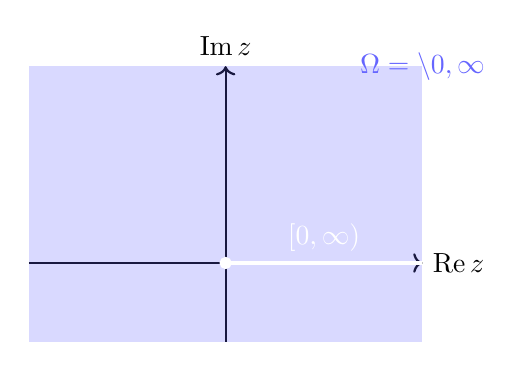
\begin{tikzpicture}
		% axes
		\draw[->, thick] (-2.5,0) -- (2.5,0) node[right] {$\Re z$};
		\draw[->, thick] (0,-1) -- (0,2.5) node[above] {$\Im z$};
		% shade domain
		\fill[blue!60, opacity=.25] (-2.5,-1) rectangle (2.5,2.5);
		\node[blue!60] at (2.5,2.5) {$\Omega=\C\setminus\intco{0,\infty}$};
		% slit: [0, +∞) on real axis
		\filldraw[white] (0,0) circle (2pt);
		\draw[white,ultra thick] (0,0) -- (2.5,0) node[midway, above] {$[0,\infty)$};
	\end{tikzpicture}
	\end{minipage}
	\end{center}
	Write $f=u+iv$ with \[
	u(x,y)=\ln r=\frac12\ln(x^2+y^2),\qquad v(x,y)=\theta=\Arg(z)\in(0,2\pi).
	\]
	On $\Omega$ the functions $u,v$ are $C^1$ and their partials are:
	\[
	u_x=\frac{x}{x^2+y^2},\quad u_y=\frac{y}{x^2+y^2},\qquad
	v_x=-\frac{y}{x^2+y^2},\quad v_y=\frac{x}{x^2+y^2}.
	\]
	Hence the Cauchy--Riemann equations hold on $\Omega$:
	\[
	u_x=v_y=\frac{x}{x^2+y^2},\qquad u_y=-v_x=\frac{y}{x^2+y^2}.
	\]
	Since these partials are continuous on $\Omega$, $f$ is analytic there. Its complex derivative is
	\[
	f'(z)=u_x+iv_x=\frac{x}{x^2+y^2}+i\!\left(-\frac{y}{x^2+y^2}\right)
	=\frac{x-iy}{x^2+y^2}=\frac{1}{x+iy}=\frac{1}{z}.
	\]
	For $g(z)=f(z^2+1)$, compute
	\begin{align*}
	z^2+1&=(x+iy)^2+1\\
	&=(x^2-y^2+2ixy) +1 \\
	&=(x^2-y^2+1)+i(2xy).
	\end{align*}
	If $x>0$ and $y>0$, then $\Im(z^2+1)=2xy>0$, so $z^2+1$ lies in the open upper half-plane $\mathbb{H}$, in particular in $\Omega$ (its argument lies in $(0,\pi)\subset(0,2\pi)$). 
	\begin{center}
	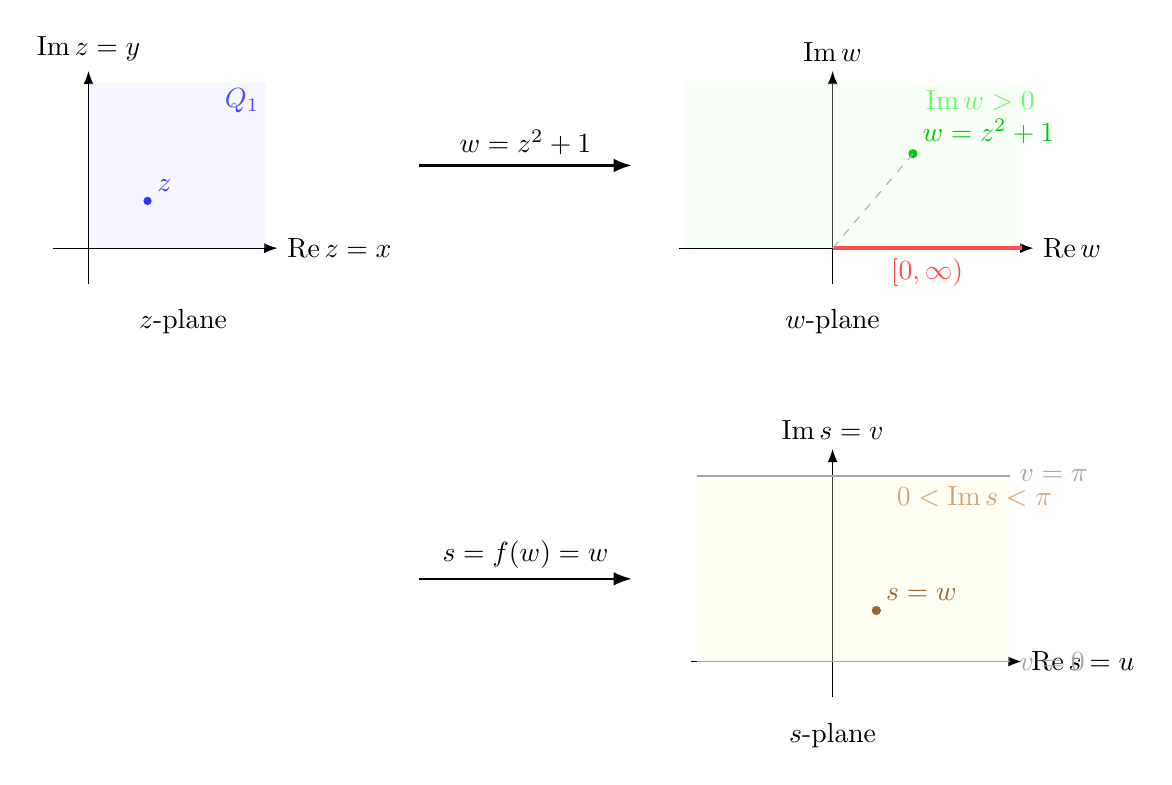
\begin{tikzpicture}[>=Latex,scale=.75]
		% ================= z-plane: domain Q =================
		\begin{scope}
			% axes
			\draw[->] (-0.6,0) -- (3.2,0) node[right] {$\Re z=x$};
			\draw[->] (0,-0.6) -- (0,3.0) node[above] {$\Im z=y$};
			\node at (1.6,-1.25) {$z$-plane};
			
			% shade first quadrant Q: x>0, y>0
			\fill[blue!12, opacity=.25] (0,0) rectangle (3.0,2.8);
			\node[blue!70] at (2.6,2.5) {$Q_1$};
			
			% sample point z = 1 + 0.8 i
			\fill[blue!80] (1.0,0.8) circle (2pt) node[above right] {$z$};
		\end{scope}
		% arrow z -> w
		\draw[->,thick] (5.6,1.4) -- (9.2,1.4) node[midway,above] {$w=z^2+1$};
		% ================= w-plane: image in upper half-plane, slit shown =================
		\begin{scope}[xshift=12.6cm]
			% axes
			\draw[->] (-2.6,0) -- (3.4,0) node[right] {$\Re w$};
			\draw[->] (0,-0.6) -- (0,3.0) node[above] {$\Im w$};
			\node at (0,-1.25) {$w$-plane};
			
			% shade upper half-plane Im w>0
			\fill[green!12, opacity=.25] (-2.5,0) rectangle (3.2,2.8);
			\node[green!60] at (2.5,2.5) {$\Im w>0$};
			
			% slit: [0, +∞) on real axis
			\draw[red!70,very thick] (0,0) -- (3.2,0) node[midway, below] {$[0,\infty)$};
%			\node[gray!70,anchor=west] at (-2.5,-0.35) {$\Omega=\C\setminus[0,\infty)$};
			% image of the sample point: z=1+0.8i -> w=(1-0.64+1)+i(2*1*0.8) = 1.36 + 1.6 i
			\fill[green!80!black] (1.36,1.60) circle (2.2pt) node[above right] {$w=z^2+1$};
			% guide from origin showing |w| and Arg(w)
			\draw[gray!60,dashed] (0,0) -- (1.36,1.60);
%			\node[gray!70] at (0.75,0.18) {$\Arg w\in(0,\pi)$};
		\end{scope}
		% arrow w -> s
		\draw[->,thick] (5.6,1.4-7) -- (9.2,1.4-7) node[midway,above] {$s=f(w)=\Log w$};
		% ================= s-plane: image strip 0<Im s<pi =================
		\begin{scope}[xshift=12.6cm, yshift=-7cm]
			% axes
			\draw[->] (-2.4,0) -- (3.2,0) node[right] {$\Re s=u$};
			\draw[->] (0,-0.6) -- (0,3.6) node[above] {$\Im s=v$};
			\node at (0,-1.25) {$s$-plane};
			% horizontal strip 0 < v < pi
			\fill[yellow!18, opacity=.25] (-2.3,0.00) rectangle (3.0,3.1416);
			\draw[gray!70] (-2.3,0.00) -- (3.0,0.00) node[right] {$v=0$};
			\draw[gray!70] (-2.3,3.1416) -- (3.0,3.1416) node[right] {$v=\pi$};
			\node[brown!70] at (2.4,2.8) {$0<\Im s<\pi$};
			% image of the sample w under Log: s = ln|w| + i Arg(w)
			% |w| ≈ sqrt(1.36^2+1.6^2) ≈ 2.100 -> ln|w| ≈ 0.741, Arg ≈ atan(1.6/1.36) ≈ 0.864
			\fill[brown!80!black] (0.741,0.864) circle (2.2pt)
			node[above right] {$s=\Log w$};
		\end{scope}
%		
%		% ================= footer: analyticity & derivative =================
%		\node[align=left] at (8.6,-0.9)
%		{\small In $Q$: $w=z^2+1$ has $\Im w=2xy>0\Rightarrow w\in\Omega$;\ \ $f=\Log$ is analytic on $\Omega$.\\
%			\small Hence $g(z)=f(z^2+1)$ is analytic on $Q$, and by chain rule
%			$\displaystyle\ g'(z)=f'(z^2+1)\cdot(2z)=\frac{2z}{z^2+1}\,.$};
%		
	\end{tikzpicture}
	\end{center}
	Thus $g$ is the composition of analytic functions on the first quadrant $Q_1$, hence analytic on $Q_1$. By the chain rule, \[
	g'(z)=f'(z^2+1)\cdot(2z)=\frac{2z}{z^2+1}\qquad (z\in Q_1).
	\]
\end{proof}
%	\item Find harmonic conjugates for $u(x,y)=2x-x^3+3xy^2$ and for $u(x,y)=\sinh x\sin y$.
%	\item If $v$ is a harmonic conjugate of $u$ and $u$ a harmonic conjugate of $v$ in $D$, show $u,v$ are constant in $D$.
%	\item Using polar CR, prove that for analytic $f=u+iv$ on $D\subset\C\setminus\{0\}$, $u$ satisfies $r^2u_{rr}+ru_r+u_{\theta\theta}=0$ (polar Laplace equation). Same for $v$.
%	\item Verify $u(r,\theta)=\ln r$ is harmonic on $r>0$, $0<\theta<2\pi$ and $v(r,\theta)=\theta$ is a harmonic conjugate.
%	\item If $f=u+iv$ is analytic on $D$, prove the level curves $u=c_1$ and $v=c_2$ intersect orthogonally at any point where $f'\neq0$.
\end{enumerate}
\newpage

\newpage
\section{Elementary Functions}
\subsection{The Exponential Function}

\defbox[Exponential Function]{
	\begin{definition}
		For $z=x+iy\in\C$, define
		\[
		e^z = e^{x+iy} = e^x(\cos y + i\sin y),
		\]
		where $y$ is in radians. We also write $\exp z$ for $e^z$.
\end{definition}}
\thmbox{
	\begin{theorem}
		For $z_1,z_2\in\C$,
		\[
		e^{z_1+z_2}=e^{z_1}e^{z_2},\qquad \frac{e^{z_1}}{e^{z_2}}=e^{z_1-z_2}.
		\]
		Moreover, $e^z$ is entire, satisfies \[
		\frac{d}{dz}e^z=e^z
		\] for all $z$, and $e^z\neq 0$ for all $z\in\C$.
\end{theorem}}

\begin{observation}
	Writing $e^z=\rho e^{i\theta}$ gives $\rho=e^x$ and $\theta=y$, hence
	\[
	|e^z|=e^x,\qquad \arg(e^z)=y+2\pi n\ (n\in\mathbb{Z}).
	\]
	Thus $e^{z+2\pi i} = e^z$, so $e^z$ is periodic with pure imaginary period $2\pi i$.
\end{observation}

\corbox[Euler's Identity]{
	\begin{corollary}
		Euler's identity is given by \[
		e^{i\pi}=-1\quad\text{equivalently,}\quad e^{i\pi}+1=0.
		\]
\end{corollary}}

\newpage
\begin{example}
	Solve $e^z=1+i$ for $z=x+iy$.
	\begin{center}
		\includegraphics[width=\textwidth]{ca-tikz/chap3-1-2.pdf}
	\end{center}
	\begin{proof}[\sol]
		Since $e^z=e^{x+iy}=e^x(\cos y+i\sin y)$ and $1+i=\sqrt{2}\left(\cos\frac{\pi}{4}+i\sin\frac{\pi}{4}\right)$, we have \[
		e^x=\sqrt{2}\quad\text{and}\quad y=\frac{\pi}{4}+2n\pi\quad (n=0,\pm1,\pm2,\cdots).
		\] Thus, \[
		x=\frac{1}{2}\ln 2\quad\text{and}\quad y=\left(2n+\frac{1}{4}\right)\pi\quad (n=0,\pm1,\pm2,\cdots)
		\] and so \[
		z=\frac{1}{2}\ln 2 + i\left(2n+\frac{1}{4}\right)\pi\quad (n=0,\pm1,\pm2,\cdots).
		\]
	\end{proof}	
\end{example}

\newpage
\subsection{The Logarithmic Function}

\begin{observation}
	To solve \[
	z=e^w
	\] for $w$ when $z\neq 0$, write $z=re^{i\theta}$, $w=u+iv$. Then $e^u=r$ and $v=\theta+2\pi n$, hence
	\[
	\log z = \ln r + i(\theta+2\pi n),\qquad n\in\mathbb{Z},
	\]
	a multiple-valued function with \[
	e^{\log z}=z
	\] for $z\neq 0$.
\end{observation}
\begin{center}
	\includegraphics[width=\textwidth]{ca-tikz/chap3-2.pdf}
\end{center}

\begin{example}
	If $z=-1-\sqrt3\,i$, then $r=2$ and $\theta=-\tfrac{2\pi}{3}$, so \[
	\log z = \ln 2 + i\Bigl(-\tfrac{2\pi}{3} + 2\pi n\Bigr),\quad n\in\mathbb{Z}.
	\]
\end{example}

\newpage
\defbox[Argument and Principal Value]{\begin{definition}
		For $z\neq 0$, the set of all arguments is $\arg z=\{\theta+2\pi n:n\in\mathbb{Z}\}$ when $z=re^{i\theta}$. The principal value $\Arg z$ is the unique $\theta$ with $-\pi<\theta\le \pi$.
\end{definition}}

\begin{observation}
	In general,
	\[
	\log(e^z)=z+2\pi i\,n,\qquad n\in\mathbb{Z}.
	\]
\end{observation}

\begin{definition}[Principal Value of the Logarithm]
	The principal value is
	\[
	\Log z = \ln r + i\theta\quad (z=re^{i\theta},\ r>0,\ -\pi<\theta<\pi).
	\]
	Then $\log z=\Log z + 2\pi i\,n$ for $n\in\mathbb{Z}$.
\end{definition}

\begin{example}
	$\log 1 = 2\pi i\,n$ with $\Log 1=0$; and $\log(-1)=(2n+1)\pi i$ with $\Log(-1)=\pi i$. The function $\Log z$ is not continuous along the negative real axis.
\end{example}
%
\subsection{Branches and Derivatives of Logarithms}

\begin{observation}
	Let $\alpha\in\R$. Restrict $\theta$ in
	\[
	\log z = \ln r + i\theta\qquad (r>0,\ \alpha<\theta<\alpha+2\pi)
	\]
	to obtain a single-valued continuous branch on that domain; it is in fact analytic there.
\end{observation}

\begin{theorem}
	For a branch as above,
	\[
	\frac{d}{dz}\log z = \frac{1}{z}\qquad(|z|>0,\ \alpha<\arg z<\alpha+2\pi).
	\]
	In particular, on the principal branch,
	\[
	\frac{d}{dz}\Log z = \frac{1}{z}\qquad(|z|>0,\ -\pi<\Arg z<\pi).
	\]
\end{theorem}

\begin{definition}[Branch, Principal Branch, Branch Cut/Point]
	A \emph{branch} of a multiple-valued $f$ is any single-valued analytic function $F$ whose values are among those of $f$. The \emph{principal branch} of $\log$ is $\Log z$ on $r>0$, $-\pi<\theta<\pi$. A \emph{branch cut} is a curve removed to render a single-valued branch; points on it are singular for that branch. The origin is a branch point for $\log$.
\end{definition}

\begin{example}
	$\Log(i^{3})=\Log(-i)=\ln 1 - i\frac{\pi}{2}=-\frac{\pi i}{2}$, while $3\Log i=3\cdot i\frac{\pi}{2}=\frac{3\pi i}{2}$. Hence $\Log(i^{3})\ne 3\Log i$.
\end{example}

\begin{theorem}
	For nonzero $z_1,z_2$,
	\[
	\log(z_1z_2)=\log z_1+\log z_2,\qquad \arg(z_1z_2)=\arg z_1+\arg z_2,
	\]
	and thus $\ln|z_1z_2|+i\arg(z_1z_2)=(\ln|z_1|+i\arg z_1)+(\ln|z_2|+i\arg z_2)$.
\end{theorem}

\begin{example}
	Let $z_1=z_2=-1$. Then $\log 1=0$, while $\log(-1)=(2n+1)\pi i$. Equality can require compatible choices of values. Using principal values everywhere may fail: $\Log(z_1z_2)=0$ but $\Log z_1+\Log z_2=2\pi i$.
\end{example}

\begin{theorem}
	For nonzero $z_1,z_2$,
	\[
	\log\!\left(\frac{z_1}{z_2}\right)=\log z_1-\log z_2.
	\]
\end{theorem}

\begin{observation}[Roots via Logarithm]
	For $z\ne 0$ and $n\in\mathbb{N}$,
	\[
	z^{1/n}=\exp\!\Bigl(\tfrac1n\log z\Bigr),
	\]
	which gives exactly the $n$ distinct $n$th roots when $k=0,1,\dots,n-1$ are taken in the angles.
\end{observation}

\subsection{Complex Exponents}

\begin{definition}[Complex Power]
	For $z\ne 0$ and $c\in\C$,
	\[
	z^{\,c}=e^{c\,\log z},
	\]
	a multiple-valued function in general.
\end{definition}

\begin{example}
	\[
	i^{-2i}=e^{-2i\log i},\qquad \log i = \ln 1 + i\Bigl(\frac{\pi}{2}+2\pi n\Bigr)=\Bigl(2n+\tfrac12\Bigr)\pi i.
	\]
	Hence $i^{-2i}=\exp\!\bigl((4n+1)\pi\bigr)$, which are real numbers.
\end{example}

\begin{observation}
	Since $1/e^z=e^{-z}$, we have $z^{-c}=\exp(-c\log z)$ and in particular $1/i^{2i}=i^{-2i}=\exp\!\bigl((4n+1)\pi\bigr)$.
\end{observation}

\begin{observation}
	Fix a branch $\log z=\ln r+i\theta$ on $\alpha<\theta<\alpha+2\pi$. Then $z^{\,c}=\exp\bigl(c\log z\bigr)$ is single-valued and analytic there, and
	\[
	\frac{d}{dz}z^{\,c}=c\,z^{\,c-1}\qquad(|z|>0,\ \alpha<\arg z<\alpha+2\pi).
	\]
	The principal value is $\mathrm{P.V.}\,z^{\,c}=\exp\bigl(c\,\Log z\bigr)$.
\end{observation}

\begin{example}
	\[
	\mathrm{P.V.}\,(-i)^i=\exp\!\bigl(i\,\Log(-i)\bigr)=\exp\!\left(i\left[\ln 1 - i\frac{\pi}{2}\right]\right)=e^{\pi/2}.
	\]
	For $z^{2/3}$ on the principal branch ($-\pi<\Arg z<\pi$),
	\[
	\mathrm{P.V.}\,z^{2/3}=r^{2/3}\!\left(\cos\frac{2\varphi}{3}+i\sin\frac{2\varphi}{3}\right)\quad(z=re^{i\varphi}).
	\]
\end{example}

\begin{example}
	Let $z_1=1+i$, $z_2=1-i$, $z_3=-1-i$. Then
	\[
	(z_1z_2)^i=e^{i\ln 2},\qquad z_1^{\,i}=e^{-\pi/4}\,e^{i(\ln 2)/2},\qquad z_2^{\,i}=e^{\pi/4}\,e^{i(\ln 2)/2},
	\]
	so $(z_1z_2)^i=z_1^{\,i}z_2^{\,i}$. But
	\[
	(z_2z_3)^i=e^{-\pi}\,e^{i\ln 2},\qquad z_3^{\,i}=e^{3\pi/4}\,e^{i(\ln 2)/2},
	\]
	whence $(z_2z_3)^i = z_2^{\,i}z_3^{\,i}e^{-2i}$, showing branch subtleties.
\end{example}

\begin{definition}[Exponential with Base $c\neq 0$]
	For fixed $c\in\C\setminus\{0\}$ and a chosen value of $\log c$, define
	\[
	c^{\,z}=e^{z\log c}.
	\]
	Then $c^{\,z}$ is entire and $\dfrac{d}{dz}c^{\,z}=c^{\,z}\log c$.
\end{definition}

\subsection{Trigonometric Functions}

\begin{definition}
	For $z\in\C$,
	\[
	\cos z = \frac{e^{iz}+e^{-iz}}{2},\qquad
	\sin z = \frac{e^{iz}-e^{-iz}}{2i}.
	\]
\end{definition}

\begin{theorem}
	The functions $\sin z$ and $\cos z$ are entire and satisfy
	\[
	\frac{d}{dz}\sin z=\cos z,\qquad \frac{d}{dz}\cos z=-\sin z,
	\]
	and remain odd/even respectively: $\sin(-z)=-\sin z$, $\cos(-z)=\cos z$. Moreover $e^{iz}=\cos z + i\sin z$.
\end{theorem}

\begin{theorem}[Formulas]
	For $z,z_1,z_2\in\C$,
	\begin{gather*}
		\sin(z_1+z_2)=\sin z_1\cos z_2+\cos z_1\sin z_2,\quad
		\cos(z_1+z_2)=\cos z_1\cos z_2-\sin z_1\sin z_2,\\
		\sin 2z=2\sin z\cos z,\quad \cos 2z=\cos^2 z-\sin^2 z,\\
		\sin(z+\tfrac{\pi}{2})=\cos z,\quad \cos(z-\tfrac{\pi}{2})=-\cos z,\\
		\sin^2 z+\cos^2 z=1,\quad \sin(z+\pi)=-\sin z,\ \cos(z+\pi)=-\cos z,\\
		\sin(z+2\pi)=\sin z,\quad \cos(z+2\pi)=\cos z.
	\end{gather*}
\end{theorem}

\begin{observation}
	For real $y$,
	\[
	\cos(iy)=\cosh y,\qquad \sin(iy)=i\sinh y.
	\]
	Writing $z=x+iy$,
	\[
	\sin z=\sin x\,\cosh y+i\cos x\,\sinh y,\quad
	\cos z=\cos x\,\cosh y - i\sin x\,\sinh y.
	\]
\end{observation}

\begin{remark}
	$\sin z$ and $\cos z$ are unbounded on $\C$.
\end{remark}

\begin{observation}[Zeros]
	$\sin z=0$ iff $z=n\pi$; $\cos z=0$ iff $z=\frac{\pi}{2}+n\pi$ for $n\in\mathbb{Z}$.
\end{observation}

\begin{definition}
	Define
	\[
	\tan z=\frac{\sin z}{\cos z},\quad \cot z=\frac{\cos z}{\sin z},\quad
	\sec z=\frac{1}{\cos z},\quad \csc z=\frac{1}{\sin z}.
	\]
\end{definition}

\begin{theorem}
	\[
	\frac{d}{dz}\tan z=\sec^2 z,\quad
	\frac{d}{dz}\sec z=\sec z\,\tan z,\quad
	\frac{d}{dz}\cot z=-\csc^2 z,\quad
	\frac{d}{dz}\csc z=-\csc z\,\cot z.
	\]
\end{theorem}

\begin{observation}
	$\tan z$ and $\sec z$ are analytic off $z=\frac{\pi}{2}+n\pi$; $\cot z$ and $\csc z$ are analytic off $z=n\pi$.
\end{observation}

\subsection{Hyperbolic Functions}

\begin{definition}
	\[
	\sinh z=\frac{e^z-e^{-z}}{2},\qquad \cosh z=\frac{e^z+e^{-z}}{2}.
	\]
\end{definition}

\begin{theorem}
	$\sinh z$ and $\cosh z$ are entire and $\dfrac{d}{dz}\sinh z=\cosh z$, $\dfrac{d}{dz}\cosh z=\sinh z$.
\end{theorem}

\begin{theorem}
	For $z=x+iy$ and $z_1,z_2\in\C$,
	\begin{gather*}
		-i\,\sinh(iz)=\sin z,\quad \cosh(iz)=\cos z,\quad
		-i\,\sin(iz)=\sinh z,\quad \cos(iz)=\cosh z,\\
		\sinh(-z)=-\sinh z,\quad \cosh(-z)=\cosh z,\quad
		\cosh^2 z-\sinh^2 z=1,\\
		\sinh(z_1+z_2)=\sinh z_1\cosh z_2+\cosh z_1\sinh z_2,\\
		\cosh(z_1+z_2)=\cosh z_1\cosh z_2+\sinh z_1\sinh z_2,\\
		\sinh z=\sinh x\cos y+i\cosh x\sin y,\\
		\cosh z=\cosh x\cos y+i\sinh x\sin y,\\
		|\sinh z|^2=\sinh^2 x+\sin^2 y,\quad |\cosh z|^2=\cosh^2 x+\cos^2 y.
	\end{gather*}
\end{theorem}

\begin{remark}
	$\sinh z$ and $\cosh z$ are periodic with period $2\pi i$.
\end{remark}

\begin{observation}[Zeros]
	$\sinh z=0$ iff $z=n\pi i$; $\cosh z=0$ iff $z=(\tfrac{\pi}{2}+n\pi)i$ ($n\in\mathbb{Z}$).
\end{observation}

\begin{definition}
	Define $\tanh z=\dfrac{\sinh z}{\cosh z}$ (analytic where $\cosh z\neq 0$). Set $\coth z=1/\tanh z$, $\operatorname{sech}z=1/\cosh z$, $\operatorname{csch}z=1/\sinh z$.
\end{definition}

\begin{theorem}
	\[
	\frac{d}{dz}\tanh z=\operatorname{sech}^2 z,\quad
	\frac{d}{dz}\operatorname{sech}z=-\operatorname{sech}z\,\tanh z,\quad
	\frac{d}{dz}\coth z=-\operatorname{csch}^2 z,\quad
	\frac{d}{dz}\operatorname{csch}z=-\operatorname{csch}z\,\coth z.
	\]
\end{theorem}

\newpage
\subsection{Inverse Trigonometric and Hyperbolic Functions}

\begin{observation}
	To define $\sin^{-1}z$, write \[
	z=\sin w=\dfrac{e^{iw}-e^{-iw}}{2i}.
	\] Then \begin{align*}
		e^{iw}-e^{-iw}&=2iz\\
		(e^{iw})^2-2iz-1&=0\\
	\end{align*} Solving the quadratic in $e^{iw}$ yields
	\[
	e^{iw}=iz+(1-z^2)^{1/2},
	\]
	where $(1-z^2)^{1/2}$ is double-valued.
\end{observation}

\defbox{
	\begin{definition}
		Multiple-valued inverses: \begin{align*}
			\sin^{-1}z&=-i\,\log\bigl[\,iz+(1-z^2)^{1/2}\bigr], \\ \\
			\cos^{-1}z&=-i\,\log\bigl[\,z+i(1-z^2)^{1/2}\bigr],\\ \\
			\tan^{-1}z&=\frac{i}{2}\log\!\left(\frac{i+z}{i-z}\right).
		\end{align*}
		With specific branches of $\sqrt{\cdot}$ and $\log$, these become single-valued and analytic on suitable domains.
\end{definition}}
\vfill
\thmbox{
	\begin{theorem}[Derivatives]
		\[
		\frac{d}{dz}\sin^{-1}z=\frac{1}{(1-z^2)^{1/2}},\qquad
		\frac{d}{dz}\cos^{-1}z=-\frac{1}{(1-z^2)^{1/2}},\qquad
		\frac{d}{dz}\tan^{-1}z=\frac{1}{1+z^2}.
		\]
\end{theorem}}

\newpage
\begin{example}
	\[
	\sin^{-1}(-i)=-i\,\log\bigl(1\pm\sqrt2\,\bigr).
	\]
	Since $\log(1+\sqrt2)=\ln(1+\sqrt2)+2\pi i\,n$ and $\log(1-\sqrt2)=\ln(\sqrt2-1)+(2n+1)\pi i$ with $\ln(\sqrt2-1)=-\ln(1+\sqrt2)$, the values of $\sin^{-1}(-i)$ are
	\[
	n\pi + i(-1)^{n+1}\ln(1+\sqrt2),\qquad n\in\mathbb{Z}.
	\]
\end{example}

\begin{observation}[Inverse Hyperbolic Functions]
	\[
	\sinh^{-1}z=\log\bigl[z+(z^2+1)^{1/2}\bigr],\quad
	\cosh^{-1}z=\log\bigl[z+(z^2-1)^{1/2}\bigr],\quad
	\tanh^{-1}z=\frac12\log\!\left(\frac{1+z}{1-z}\right).
	\]
\end{observation}
\newpage
\subsection{Exercises}
\begin{enumerate}[\bfseries 1.]
	\item Show that $f(z)=\exp(\overline{z})$ is not analytic anywhere.
	
	\noindent 
	\textit{(Hint: use the Cauchy--Riemann equations.)}
	\begin{proof}[\sol]
		(\textbf{Proof via Cauchy--Riemann equations}) Write \(z=x+iy\). Then \[
		f(z)=e^{\overline z}=e^{x-iy}=e^{x}\bigl(\cos y-i\sin y\bigr),
		\] so \[
		u(x,y)=e^{x}\cos y,\qquad v(x,y)=-e^{x}\sin y.
		\] Then \[
		u_x=e^{x}\cos y,\quad u_y=-e^{x}\sin y,\qquad
		v_x=-e^{x}\sin y,\quad v_y=-e^{x}\cos y.
		\] If \(f\) is complex differentiable at \((x,y)\), the Cauchy--Riemann equations would hold: \[
		u_x=v_y \quad\text{and}\quad u_y=-\,v_x.
		\] That is, \begin{align*}
			u_x=v_y&\implies e^x\cos y=-e^x\cos y&\implies \cos y=0, \\
			u_y=-v_x&\implies -e^x\sin y=e^x\sin y&\implies \sin y=0.
		\end{align*}
		There is no \(y\in\mathbb{R}\) with \(\cos y=0\) and \(\sin y=0\) simultaneously. Hence the Cauchy--Riemann equations fail at every point, so \(f\) is nowhere analytic.
		
	\medskip\noindent
	(\textbf{Proof via Wirtinger derivatives})
		Using \(\partial/\partial z=\tfrac12(\partial_x- i\,\partial_y)\) and
		\(\partial/\partial\overline z=\tfrac12(\partial_x+ i\,\partial_y)\),
		one checks directly that \[
		\frac{\partial f}{\partial z}=0,
		\qquad
		\frac{\partial f}{\partial \overline z}=e^{\overline z}\neq 0\ \text{ for all } z.
		\]
		A function is holomorphic iff \(\partial f/\partial \overline z\equiv 0\) on its domain. Since this is not the case, \(f\) is nowhere holomorphic.
	\end{proof}
	%\begin{remark}
	%		The map \(z\mapsto e^{\overline z}\) is \emph{anti-holomorphic}: the composition \(z\mapsto \overline z\) (conjugation) with the holomorphic \(w\mapsto e^{w}\). It is holomorphic only on the empty set.
	%	\end{remark}
	\newpage
	\item Let $f(z)=u(x,y)+iv(x,y)$ be analytic in a domain $D$. Show that \[
		U(x,y)=e^{u(x,y)}\cos v(x,y),\qquad V(x,y)=e^{u(x,y)}\sin v(x,y)
		\] are harmonic in $D$, and that $V$ is a harmonic conjugate of $U$.
	\begin{proof}[\sol]
		Since $f$ is analytic on $D$, the composition
		\[
		F(z):=e^{f(z)}=e^{u(x,y)}\big(\cos v(x,y)+i\sin v(x,y)\big)=U(x,y)+iV(x,y)
		\]
		is analytic on $D$ (composition of analytic maps). It follows that
		$U=\Re F$ and $V=\Im F$ are harmonic and satisfy the Cauchy--Riemann equations.
%		For completeness, we verify the CR equations directly and then deduce harmonicity.
		\begin{center}
		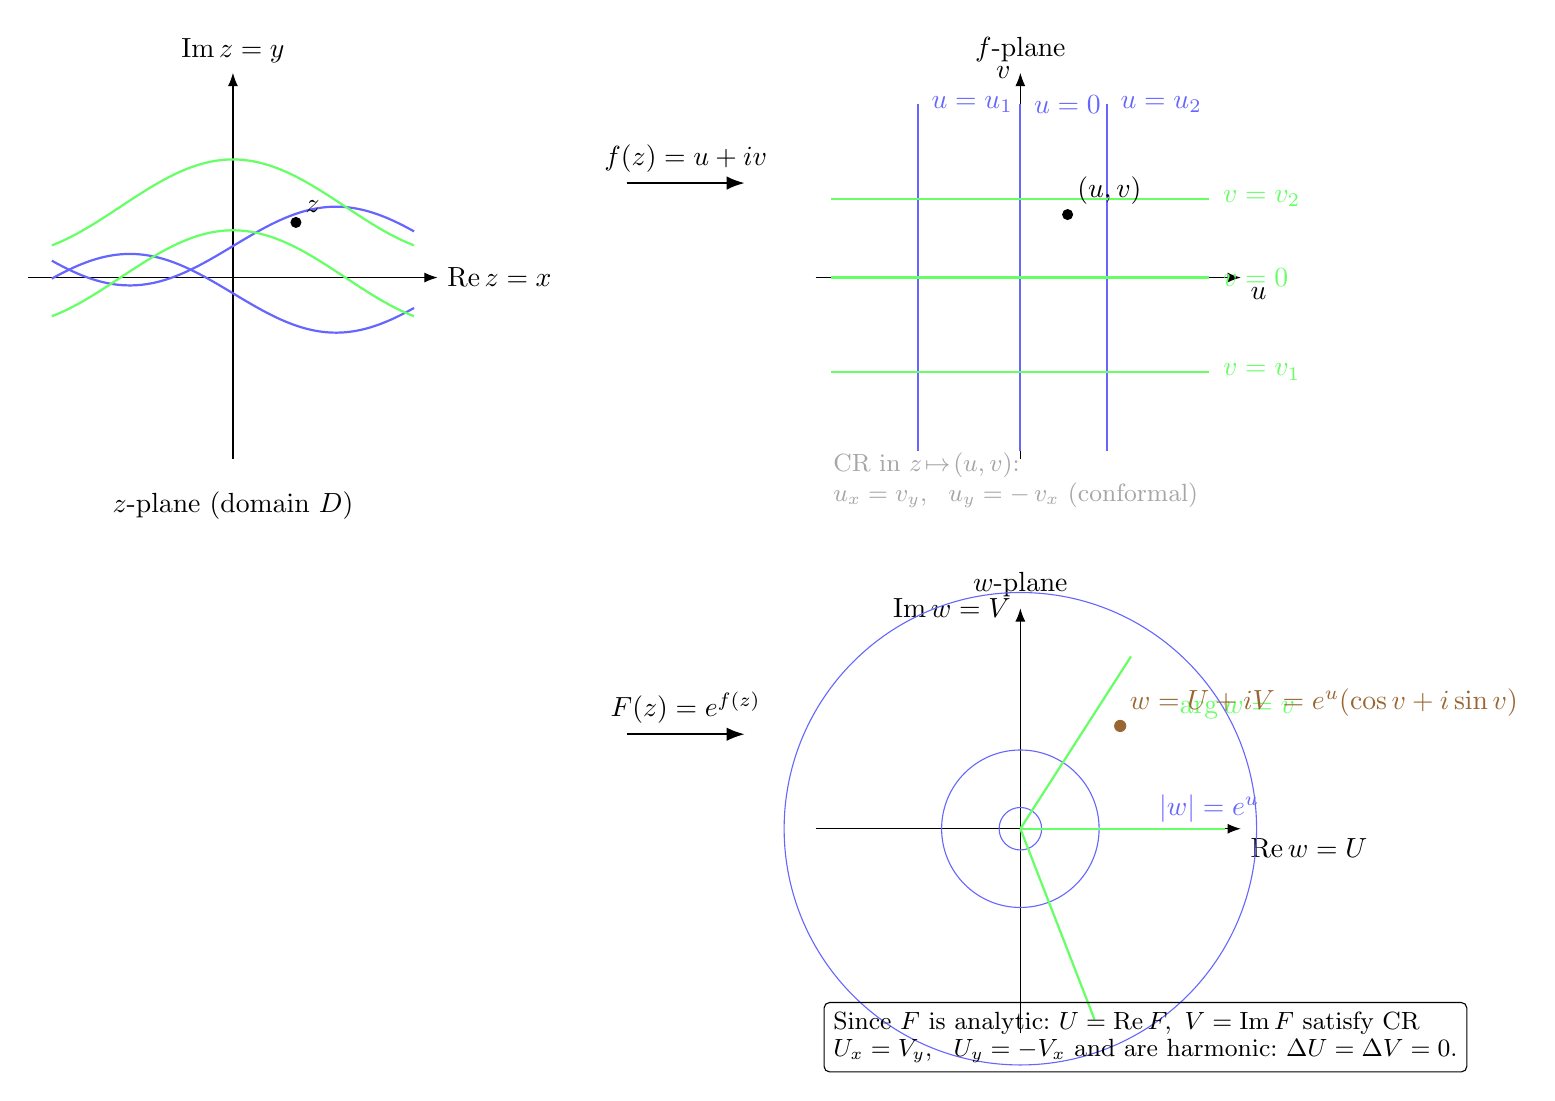
\begin{tikzpicture}[>=Latex,scale=1]
			% ================= z-plane =================
			\begin{scope}
				% axes
				\draw[->] (-2.6,0) -- (2.6,0) node[right] {$\Re z=x$};
				\draw[->] (0,-2.3) -- (0,2.6) node[above] {$\Im z=y$};
				\node at (0,-2.9) {$z$-plane (domain $D$)};
				
				% suggestive orthogonal families u=const (blue) and v=const (green) pulled back by f
				% (schematic curves—just to show orthogonality/conformality)
				\draw[blue!60,thick,domain=-2.3:2.3,samples=100,smooth] plot(\x,{0.5*sin(1.2*\x r)+0.4});
				\draw[blue!60,thick,domain=-2.3:2.3,samples=100,smooth] plot(\x,{-0.5*sin(1.2*\x r)-0.2});
				\draw[green!60,thick,domain=-2.3:2.3,samples=100,smooth] plot(\x,{0.6*cos(1.1*\x r)});
				\draw[green!60,thick,domain=-2.3:2.3,samples=100,smooth] plot(\x,{0.6*cos(1.1*\x r)+0.9});
				
				% sample point z0
				\fill[black] (0.8,0.7) circle (2pt) node[above right] {$z$};
			\end{scope}
			
			% arrow to (u,v)-plane
			\draw[->,thick] (5.0,1.2) -- (6.5,1.2) node[midway,above] {$f(z)=u+iv$};
			
			% ================= (u,v)-plane =================
			\begin{scope}[xshift=10cm]
				% axes
				\draw[->] (-2.6,0) -- (2.8,0) node[below right] {$u$};
				\draw[->] (0,-2.3) -- (0,2.6) node[left] {$v$};
				\node at (0,2.9) {$f$-plane};
				
				% horizontals u=const
				\foreach \uu/\lab in {-1.3/{$u=u_1$},0/{$u=0$},1.1/{$u=u_2$}}{
					\draw[blue!60,thick] (\uu,-2.2) -- (\uu,2.2);
					\node[blue!60,anchor=west] at (\uu+0.05,2.2) {\lab};
				}
				% verticals v=const
				\foreach \vv/\lab in {-1.2/{$v=v_1$},0/{$v=0$},1.0/{$v=v_2$}}{
					\draw[green!60,thick] (-2.4,\vv) -- (2.4,\vv);
					\node[green!60,anchor=west] at (2.45,\vv) {\lab};
				}
				
				% sample point (u0,v0) and its small orthonormal frame
				\fill (0.6,0.8) circle (2pt) node[above right] {$(u,v)$};
				% Jacobian of exp at (u,v) is E*[ [cos v, -sin v],[sin v, cos v] ]
				\node[gray!70,align=left,anchor=north west] at (-2.5,-2.1)
				{\small CR in $z\!\mapsto\!(u,v)$:\\[-1pt]
					\small $u_x=v_y,\ \ u_y=-\,v_x$ (conformal)};
			\end{scope}
			% arrow to w-plane
			\draw[->,thick] (5,1.2-7) -- (6.5,1.2-7) node[midway,above] {$F(z)=e^{f(z)}$};
			% ================= w-plane =================
			\begin{scope}[xshift=10cm, yshift=-7cm]
				% axes
				\draw[->] (-2.6,0) -- (2.8,0) node[below right] {$\Re w=U$};
				\draw[->] (0,-2.6) -- (0,2.8) node[left] {$\Im w=V$};
				\node at (0,3.1) {$w$-plane};
				
				% image of u-const: circles of radius e^u
				\draw[blue!60] (0,0) circle (0.27); % e^{-1.3} ~ 0.27
				\draw[blue!60] (0,0) circle (1.00); % e^{0}   = 1
				\draw[blue!60] (0,0) circle (3.00); % e^{~1.1}\approx 3.0 (schematic)
				\node[blue!60] at (2.4,0.25) {$|w|=e^{u}$};
				
				% image of v-const: rays with angle v
				\foreach \ang/\txt in {-1.2/{$v_1$},0/{$0$},1.0/{$v_2$}}{
					\draw[green!60,thick] (0,0) -- ({2.6*cos(\ang r)},{2.6*sin(\ang r)});
				}
				\node[green!60,anchor=west] at (1.9,1.5) {$\arg w=v$};
				
				% image point
				% choose u0=0.6, v0=0.8 -> radius e^{0.6}\approx 1.82, angle 0.8
				\fill[brown!80!black] ({1.82*cos(0.8 r)},{1.82*sin(0.8 r)}) circle (2.2pt)
				node[above right] {$w=U+iV=e^{u}(\cos v+i\sin v)$};
				
				% CR & harmonic box
				\node[draw,rounded corners=2pt,align=left,anchor=north west] at (-2.5,-2.2)
				{\small Since $F$ is analytic:\ $U=\Re F,\ V=\Im F$ satisfy CR\\[-2pt]
					\small $U_x=V_y,\ \ U_y=-V_x$ and are harmonic:\ $\Delta U=\Delta V=0$.};
			\end{scope}
		\end{tikzpicture}
		\end{center}
		Note that
		\begin{align*}
			U_x &= e^{u(x,y)}\,(u_x\cos v - v_x\sin v), &\qquad
			U_y &= e^{u(x,y)}\,(u_y\cos v - v_y\sin v),\\
			V_x &= e^{u(x,y)}\,(u_x\sin v + v_x\cos v), &\qquad
			V_y &= e^{u(x,y)}\,(u_y\sin v + v_y\cos v).
		\end{align*}
		Because $f$ is analytic, $u,v$ satisfy the CR equations $u_x=v_y$ and $u_y=-\,v_x$. Substituting,
		\begin{align*}
			U_x &= e^{u(x,y)}\,(v_y\cos v - v_x\sin v)=V_y,\\
			U_y &= e^{u(x,y)}\,(-v_x\cos v - v_y\sin v)= -\,V_x.
		\end{align*}
		Thus $U_x=V_y$ and $U_y=-V_x$, i.e.\ $V$ is a harmonic conjugate of $U$.
		
		To show harmonicity, differentiate the CR relations and use equality of mixed partials:
		\[
		U_{xx} = (V_y)_x = V_{yx},\qquad
		U_{yy} = (-V_x)_y = -V_{xy}.
		\]
		Hence $\Delta U:=U_{xx}+U_{yy}=V_{yx}-V_{xy}=0$. Similarly,
		\[
		V_{xx} = (-U_y)_x = -U_{yx},\qquad
		V_{yy} = (U_x)_y = U_{xy},
		\]
		so $\Delta V:=V_{xx}+V_{yy}=-U_{yx}+U_{xy}=0$. Therefore $U$ and $V$ are harmonic on $D$, and $V$ is a harmonic conjugate of $U$.
	\end{proof}
	\newpage
	\item Show that $f(z)=\Log(z-i)$ is analytic except on portion $x\leq 0$ of the line $y=1$ and that the function
		\[
		f(z)=\frac{\Log(z+4)}{z^2+i}
		\] is analytic everywhere except at the points $\pm{(1-i)}/{\sqrt2}$ and on the portion $x\leq -4$ of the real axis.
	\begin{proof}[\sol]
		Consider $\Log\; z=\ln|z|+i\Arg\; z$, the principal branch of the complex logarithm,
		with $\Arg\; z\in(-\pi,\pi)$, so that $\Log$ is analytic on \begin{align*}
			\mathbb{C}\setminus(-\infty,0] &= \C\setminus\set{z\in\C:\Re z\leq 0\land\Im z=0}\\
			&=\{\, z\in\mathbb{C} : \Re z>0\lor \Im z\neq 0\,\}.
		\end{align*} Then
		\begin{enumerate}[(1)]
			\item Since $\Log$ is analytic on $\mathbb{C}\setminus(-\infty,0]$ and the map $z\mapsto z-i$ is entire,
			the composition $z\mapsto \Log(z-i)$ is analytic precisely where $z-i\notin(-\infty,0]$.
			Equivalently, \begin{align*}
				z-i\in(-\infty,0] &\iff \Re(z-i)\le 0 \text{ and } \Im(z-i)=0 \\
				&\iff \Re(x+i(y-1))=x\le 0 \text{ and } \Im(x+i(y-1))=y-1=0.
			\end{align*}
			That is, $f(z):=\Log(z-i)$ is analytic on $\mathbb{C}\setminus\{\,x+iy:\; x\le 0,\ y=1\}$. 
	%i.e. it is analytic except on the portion $x\le0$ of the line $y=1$.
			\begin{center}
				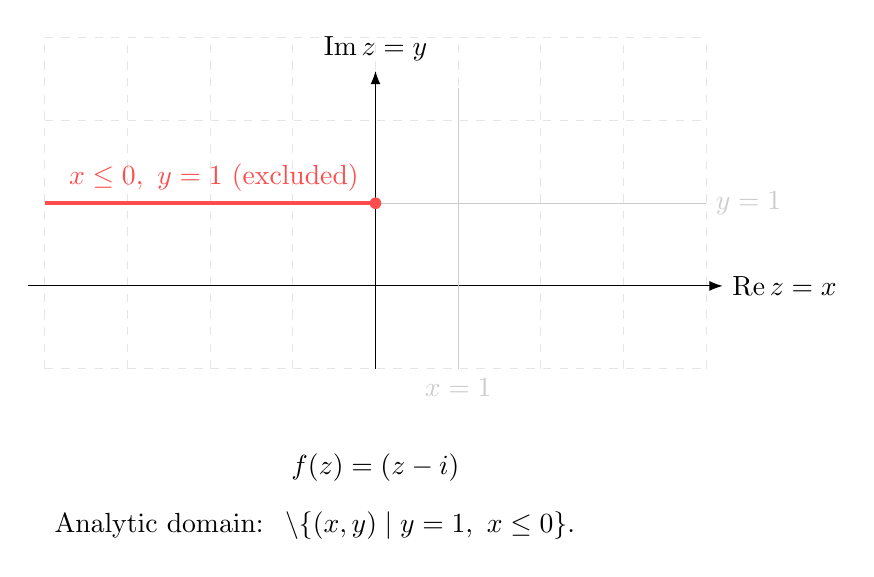
\begin{tikzpicture}[>=Latex,scale=1.05]
					\draw[gray!20, dashed] (-4,-1) grid (4,3);
					% axes
					\draw[->] (-4.2,0) -- (4.2,0) node[right] {$\Re z=x$};
					\draw[->] (0,-1) -- (0,2.6) node[above] {$\Im z=y$};
					\node at (0,-2.2) {$f(z)=\Log(z-i)$};
					% a few reference gridlines for context
					\draw[gray!40] (-4.0, 1.0) -- (4.0, 1.0) node[right] {$y=1$};
					\draw[gray!40] ( 1.0,2.4) -- ( 1.0, -1) node[below] {$x=1$};
					% branch cut in z-plane: y = 1, x <= 0  (comes from w=z-i \in (-\infty,0])
					\draw[ultra thick,red!70] (-4.0,1.0) -- (0.0,1.0) node[midway,above] {$\;x\le 0,\ y=1$ (excluded)};
					\fill[red!70] (0.0,1.0) circle (2pt); % includes endpoint x=0
					% legend
					\node[align=left,anchor=west] at (-4.0,-2.9)
					{Analytic domain: $\ \C \setminus \{(x,y)\mid y=1,\ x\le 0\}$.};
				\end{tikzpicture}
			\end{center}
			\item The numerator $z\mapsto \Log(z+4)$ is analytic wherever $z+4\notin(-\infty,0]$, i.e., $z\notin\intoc{-\infty,-4}$. In other words, $\Log(z+4)$ is analytic on \[
			\C\setminus\intoc{-\infty,-4}=\C\setminus\set{z\in\C:\Re z\leq -4\land \Im z = 0}=\set{z\in\C:\Re z>-4\lor \Im z\neq 0 }
			\] $\C\setminus\intoc{-\infty}$ for
			$z\notin(-\infty,-4]$, which is the portion $x\le -4$ of the real axis.
			The denominator $z^2+i$ vanishes exactly at the zeros of $z^2=-i$, namely
			\[
			z=\pm(-i)^{1/2}=\pm e^{-i\pi/4}=\pm\frac{1-i}{\sqrt2}.
			\]
			Therefore $g$ is analytic on the domain where the numerator is analytic and the denominator is nonzero, i.e.
			\[
			\mathbb{C}\setminus\Big( (-\infty,-4]\ \cup\ \{\pm\tfrac{1-i}{\sqrt2}\}\Big),
			\]
			which is exactly the stated set.
			
			$g(z):=\dfrac{\Log(z+4)}{z^2+i}$ is analytic on
			\[
			\mathbb{C}\setminus\Big(\{\,x+iy:\; y=0,\ x\le -4\,\}\ \cup\ \{\pm\tfrac{1-i}{\sqrt2}\}\Big),
			\]
			i.e. everywhere except at the branch cut $x\le -4$ on the real axis and at the two points $\pm{(1-i)}/{\sqrt2}$.
			
			\begin{center}
				\begin{tikzpicture}[>=Latex,scale=1.05]
					\draw[gray!20, dashed] (-4,-4) grid (4,4);
					% axes
					\draw[->] (-6.2,0) -- (4.2,0) node[right] {$\Re z=x$};
					\draw[->] (0,-3.2) -- (0,3.2) node[above] {$\Im z=y$};
					\node at (0,-3.5) {$g(z)=\dfrac{\Log(z+4)}{z^2+i}$};
					% branch cut from Log(z+4): real axis x <= -4
					\draw[very thick,red!70] (-6.0,0.0) -- (-4.0,0.0) node[midway,above] {$\ (-\infty,-4]$ (excluded)};
					\fill[red!70] (-4.0,0.0) circle (2pt); % includes endpoint x=-4
					% poles from z^2+i=0: z = ±(1 - i)/√2  ≈ (±0.7071, ∓0.7071)
					\draw[red!80,very thick] ( 0.7071,-0.7071) +(0.12,0.12) -- +(-0.12,-0.12);
					\draw[red!80,very thick] ( 0.7071,-0.7071) +(-0.12,0.12) -- +(0.12,-0.12);
					\node[red!80,anchor=west] at (0.78,-0.70) {$\ \ \tfrac{1-i}{\sqrt2}$};
					\draw[red!80,very thick] (-0.7071, 0.7071) +(0.12,0.12) -- +(-0.12,-0.12);
					\draw[red!80,very thick] (-0.7071, 0.7071) +(-0.12,0.12) -- +(0.12,-0.12);
					\node[red!80,anchor=east] at (-0.78,0.70) {$\tfrac{-1+i}{\sqrt2}\ $};
					\draw[red!80,very thick, dotted] ( 0.7071,0) -- ( 0.7071,-0.7071);
					\draw[red!80,very thick, dotted] ( 0,-0.7071) -- ( 0.7071,-0.7071);
					\draw[red!80,very thick, dotted] ( -0.7071,0.7071) -- ( -0.7071,0);
					\draw[red!80,very thick, dotted] ( 0,0.7071) -- ( -0.7071,0.7071);
%					% legend
%					\node[align=left,anchor=west] at (-6.0,-2.7)
%					{Analytic domain: $\ \C\setminus\big((-\infty,-4]\cup\{\pm\tfrac{1-i}{\sqrt2}\}\big)$.};
				\end{tikzpicture}
			\end{center}
		\end{enumerate}
	\end{proof}
	\newpage
	\item Show that the function $\ln(x^2+y^2)$ is harmonic in every domain that does not contain the origin.
	\begin{proof}[\sol]
%		We need to show that $u(x,y) = \ln(x^2 + y^2)$
%		satisfies Laplace’s equation \[
%		u_{xx} + u_{yy} = 0
%		\] at every point $(x,y)\neq(0,0)$. 
		For $(x,y)\neq(0,0)$, we can differentiate: \begin{align*}
		u_x &= \frac{\partial}{\partial x}\ln(x^2 + y^2) = \frac{2x}{x^2 + y^2},\\
		u_y &= \frac{\partial}{\partial y}\ln(x^2 + y^2) = \frac{2y}{x^2 + y^2}.
		\end{align*} And then \begin{align*}
		u_{xx}
		&= \frac{2(x^2 + y^2) - 2x\cdot 2x}{(x^2 + y^2)^2}
		= \frac{2(x^2 + y^2) - 4x^2}{(x^2 + y^2)^2}
		= \frac{-2x^2 + 2y^2}{(x^2 + y^2)^2} \\
		u_{yy}
		&= \frac{2(x^2 + y^2) - 2y\cdot 2y}{(x^2 + y^2)^2}
		= \frac{2(x^2 + y^2) - 4y^2}{(x^2 + y^2)^2}
		= \frac{2x^2 - 2y^2}{(x^2 + y^2)^2}.
		\end{align*}	
		Now compute the Laplacian: \[
		u_{xx} + u_{yy}
		= \frac{-2x^2 + 2y^2}{(x^2 + y^2)^2}+
		\frac{2x^2 - 2y^2}{(x^2 + y^2)^2}
		= \frac{(-2x^2 + 2y^2) + (2x^2 - 2y^2)}{(x^2 + y^2)^2}
		= \frac{0}{(x^2 + y^2)^2}
		= 0
		\] for all $(x,y)\neq(0,0)$.
%		So $\ln(x^2 + y^2)$ is harmonic at every point where it is twice continuously differentiable --- that is, on any domain that does not contain the origin (since at ((0,0)) the function is not even defined, and our derivatives blow up).	
%		Therefore, **(\ln(x^2 + y^2)) is harmonic in every domain that does not contain the origin.**
		
		\medskip\noindent
		(\textbf{Proof via Wirtinger-operator})
		Let $z=x+iy$ and
		\[
		u(x,y)=\ln(x^2+y^2)=\ln(\abs{z}^2)=\ln(z\bar z).
		\]
		Recall the Wirtinger operators $
		\partial:=\tfrac12(\partial_x-i\,\partial_y)$ and
		$\bar\partial:=\tfrac12(\partial_x+i\,\partial_y),$
		so that the Laplacian satisfies
		\[
		\Delta=\partial_{xx}+\partial_{yy}=4\,\partial\bar\partial=4\,\bar\partial\partial.
		\]
		On $\mathbb{C}\setminus\{0\}$ the chain rule gives \begin{align*}
		\partial u
		&=\partial\big(\ln(z\bar z)\big)
		=\frac{1}{z\bar z}\,\partial(z\bar z)
		=\frac{1}{z\bar z}\,\bar z
		=\frac{1}{z},\\
		\bar\partial u
		&=\bar\partial\big(\ln(z\bar z)\big)
		=\frac{1}{z\bar z}\,\bar\partial(z\bar z)
		=\frac{1}{z\bar z}\,z
		=\frac{1}{\bar z}.
		\end{align*}
		Therefore,
		\[
		\Delta u
		=4\,\partial\bar\partial u
		=4\,\partial\!\left(\frac{1}{\bar z}\right)
		=0\qquad\text{on }\mathbb{C}\setminus\{0\}.
		\]
%		since $\partial(1/\bar z)=0$ away from the origin (equivalently, $\bar\partial(1/z)=0$).
%		Hence $u(x,y)=\ln(x^2+y^2)$ is harmonic on any domain not containing $0$.
%		\emph{Remark (distributional):} Globally, $\Delta\ln|z|^2=4\pi\,\delta_0$; the failure of harmonicity is a point mass at the origin.
	\end{proof}
	\newpage
	\item Show that neither $\sin\bar z$ nor $\cos\bar z$ is an analytic function of $z$ anywhere.
	
	\textit{(Hint: use the Cauchy--Riemann equation.)}
	\begin{proof}[\sol]
		(\textbf{Proof via CR-equations})
		Write \(z=x+iy\).
		\begin{enumerate}[(1)]
			\item Let \[
			f(z)=\sin(\overline z)=\sin(x-iy)=\sin(x)\cos(iy)-\cos x\sin(iy)=\sin x\cosh y - i\,\cos x\sinh y
			\] then \[
			u(x,y)=\sin x\cosh y,\qquad v(x,y)=-\cos x\sinh y.
			\]
			Compute the partials:
			\[
			u_x=\cos x\cosh y,\quad u_y=\sin x\sinh y,\qquad
			v_x=\sin x\sinh y,\quad v_y=-\cos x\cosh y.
			\]
			The Cauchy--Riemann (CR) equations \(u_x=v_y\) and \(u_y=-v_x\) become
			\[
			\cos x\cosh y=-\cos x\cosh y \quad\Longrightarrow\quad \cos x\cosh y=0,
			\]
			\[
			\sin x\sinh y=-\sin x\sinh y \quad\Longrightarrow\quad \sin x\sinh y=0.
			\]
			Since \(\cosh y\neq 0\) for all \(y\), the first forces \(\cos x=0\). Then the second gives either
			\(\sin x=0\) (impossible simultaneously with \(\cos x=0\)) or \(\sinh y=0\), i.e.\ \(y=0\).
			Hence the CR equations can hold only at isolated points with \(y=0\) and \(\cos x=0\) (i.e.\ \(x=\tfrac{\pi}{2}+k\pi\)).
			They \emph{cannot} hold on any open set. Therefore \(f\) is not analytic anywhere.
			\item \(g(z)=\cos(\overline z)=\cos(x-iy)=\cos x\cosh y + i\,\sin x\sinh y\).
			Thus
			\[
			u(x,y)=\cos x\cosh y,\qquad v(x,y)=\sin x\sinh y.
			\]
			Compute the partials:
			\[
			u_x=-\sin x\cosh y,\quad u_y=\cos x\sinh y,\qquad
			v_x=\cos x\sinh y,\quad v_y=\sin x\cosh y.
			\]
			The CR equations give
			\[
			u_x=v_y \ \Longrightarrow\ -\sin x\cosh y=\sin x\cosh y \ \Longrightarrow\ \sin x\cosh y=0,
			\]
			\[
			u_y=-v_x \ \Longrightarrow\ \cos x\sinh y=-\cos x\sinh y \ \Longrightarrow\ \cos x\sinh y=0.
			\]
			Again, since \(\cosh y\neq 0\), the first forces \(\sin x=0\); then the second forces either \(\cos x=0\) (incompatible)
			or \(\sinh y=0\), i.e.\ \(y=0\). Thus CR can hold only at isolated points with \(y=0\) and \(\sin x=0\) (i.e.\ \(x=k\pi\)),
			and not on any open set. Therefore \(g\) is not analytic anywhere.
		\end{enumerate}

		\medskip\noindent
		(\textbf{Proof via Wirtinger-operators})
		Recall the Wirtinger operators
		\[
		\partial=\tfrac12(\partial_x-i\,\partial_y),\qquad
		\bar\partial=\tfrac12(\partial_x+i\,\partial_y),
		\]
		and the criterion: a \(C^1\) function \(F\) is holomorphic on an open set iff \(\bar\partial F\equiv 0\) there.
		
		Let \(h(w)=\sin w\). Then \(f_1(z):=\sin(\overline z)=h(\overline z)\) satisfies
		\[
		\partial f_1(z)=0,\qquad \bar\partial f_1(z)=h'(\overline z)=\cos(\overline z).
		\]
		Similarly, with \(h(w)=\cos w\), \(f_2(z):=\cos(\overline z)\) satisfies
		\[
		\partial f_2(z)=0,\qquad \bar\partial f_2(z)=h'(\overline z)=-\sin(\overline z).
		\]
		In each case, \(\bar\partial f_j\) is \emph{not} identically zero on any open set (its zero set is discrete). Hence neither
		\(f_1\) nor \(f_2\) is holomorphic on any nonempty open set; i.e. they are nowhere analytic.
		
		\emph{Remark.} At isolated points where \(\cos(\overline z)=0\) (respectively \(\sin(\overline z)=0\)), the complex
		difference quotient may happen to have limit \(0\); however, analyticity requires \(\bar\partial f\equiv 0\) on a neighborhood, which fails here.
	\end{proof}
	\item Show that $\cosh^2 z-\sinh^2 z=1$ and $\sinh z+\cosh z=e^z$.
	\begin{proof}[\sol]
	Recall the exponential definitions (valid for all $z\in\mathbb{C}$):
	\[
	\cosh z=\frac{e^{z}+e^{-z}}{2},\qquad
	\sinh z=\frac{e^{z}-e^{-z}}{2}.
	\]
	
	\medskip
	\noindent\textbf{(1) $\cosh^2 z-\sinh^2 z=1$.}
	\[
	\cosh^2 z-\sinh^2 z
	=\left(\frac{e^{z}+e^{-z}}{2}\right)^{\!2}
	-\left(\frac{e^{z}-e^{-z}}{2}\right)^{\!2}
	=\frac{(e^{z}+e^{-z})^2-(e^{z}-e^{-z})^2}{4}.
	\]
	Expanding,
	\[
	(e^{z}+e^{-z})^2-(e^{z}-e^{-z})^2
	=e^{2z}+2+e^{-2z}-(e^{2z}-2+e^{-2z})=4,
	\]
	so $\cosh^2 z-\sinh^2 z=\frac{4}{4}=1$.
	
	\medskip
	\noindent\textbf{(2) $\sinh z+\cosh z=e^{z}$.}
	\[
	\sinh z+\cosh z
	=\frac{e^{z}-e^{-z}}{2}+\frac{e^{z}+e^{-z}}{2}
	=e^{z}.
	\]
	\end{proof}
\end{enumerate}


\newpage
\section{Integrals}

\subsection{Definite Integrals of Complex-Valued Functions}

\defbox[Derivative]{
	\begin{definition}\label{def:derivative}
		If $w(t)=u(t)+iv(t)$ with real-valued $u,v$, the derivative is
		\[
		\dv{t}w(t)=w'(t)=u'(t)+iv'(t),
		\]
		whenever $u'$ and $v'$ exist. If $z_0=x_0+iy_0$ is constant, then
		\[
		\dv{t}\big[z_0w(t)\big]=z_0\,w'(t),\qquad
		\dv{t}\,e^{z_0t}=z_0\,e^{z_0t}.
		\]
\end{definition}}

\begin{observation}[No mean value theorem for derivatives]
	If $w(t)$ is continuous on $[a,b]$ and differentiable on $(a,b)$, there need \emph{not} exist $c\in(a,b)$ with
	\[
	w'(c)=\frac{w(b)-w(a)}{b-a}.
	\]
	For $w(t)=e^{it}$ on $[0,2\pi]$, we have $\abs{w'(t)}=1$ but $[w(2\pi)-w(0)]/(2\pi)=0$. 
\end{observation}

\begin{definition}[Definite integral]\label{def:defint}
	For $w(t)=u(t)+iv(t)$,
	\[
	\int_a^b w(t)\,dt
	=\int_a^b u(t)\,dt \;+\; i\int_a^b v(t)\,dt,
	\]
	with analogous definitions for improper integrals.
\end{definition}

\begin{example}
	\[
	\int_0^1 (1+it)^2\,dt
	=\int_0^1(1-t^2)\,dt+i\int_0^1 2t\,dt
	=\frac{2}{3}+i.
	\]
\end{example}

\begin{theorem}[Additivity]
	For $a\le c\le b$,
	\[
	\int_a^b w(t)\,dt=\int_a^c w(t)\,dt+\int_c^b w(t)\,dt.
	\]
\end{theorem}

\newpage
\thmbox[Fundamental Theorem of Calculus]{
	\begin{theorem}\label{thm:FTC}
		If $W'(t)=w(t)$ and $W,w$ are continuous on $[a,b]$, then \[
		\int_a^b w(t)\,dt=W(b)-W(a).
		\]
\end{theorem}}
\begin{example}
	Since $\dv{t}\!\big(e^{it}/i\big)=e^{it}$,
	\[
	\int_0^{\pi/4}e^{it}\,dt=\left[\frac{e^{it}}{i}\right]_{0}^{\pi/4}
	=\frac{1}{\sqrt2}+i\!\left(1-\frac{1}{\sqrt2}\right).
	\]
\end{example}

\begin{remark}[No mean value theorem for integrals]
	There need not be $c\in(a,b)$ with \[
	w(c)=\frac{1}{b-a}\int_a^bw(t)\,dt
	\] when $w$ is complex-valued.
\end{remark}

\subsection{Contours}

\defbox[Arc]{
	\begin{definition}\label{def:arc}
		An \emph{arc} $C$ is a set $z(t)=x(t)+iy(t)$, $a\le t\le b$, where $x,y$ are continuous.
\end{definition}}

\begin{definition}[Simple arc / Jordan curve]
	$C$ is \emph{simple} if $z(t_1)\ne z(t_2)$ for $t_1\ne t_2$. If $C$ is simple with $z(a)=z(b)$, it is a \emph{simple closed curve} (Jordan curve). Positive orientation is counterclockwise.
\end{definition}

\begin{example}
	The polygonal line from $0$ to $1+i$ to $2+i$ is a simple arc; $z=e^{i\theta}$, $0\le\theta\le2\pi$, is a positively oriented unit circle; $z=z_0+Re^{i\theta}$ is a circle centered at $z_0$ of radius $R$. Traversing $z=e^{-i\theta}$ reverses orientation; $z=e^{i2\theta}$ traverses the unit circle twice.
\end{example}

\begin{observation}[Arc length]
	If $z'(t)=x'(t)+iy'(t)$ is continuous on $[a,b]$, then
	\[
	L(C)=\int_a^b \abs{z'(t)}\,dt,\qquad
	\abs{z'(t)}=\left([x'(t)]^2+[y'(t)]^2\right)^{1/2}.
	\]
	The unit tangent is $T=z'(t)/\abs{z'(t)}$ where $z'(t)\neq0$; such an arc is \emph{smooth}.
\end{observation}

\defbox[Smooth arc and contour]{
	\begin{definition}\label{def:contour}
		An arc is \emph{smooth} if $z'(t)$ is continuous on $[a,b]$ and nonzero on $(a,b)$. A \emph{contour} (piecewise smooth arc) is a finite concatenation of smooth arcs. A contour with identical initial and final points is a \emph{simple closed contour}.
\end{definition}}

\thmbox[Jordan Curve Theorem]{
	\begin{theorem}
		A simple closed curve $C$ is the boundary of exactly two domains: a bounded interior and an unbounded exterior.
\end{theorem}}

\subsection{Contour Integrals}

\defbox[Contour integral]{
	\begin{definition}\label{def:contint}
		If $C$ is given by $z=z(t)$, $a\le t\le b$, and $f$ is (piecewise) continuous on $C$, define
		\[
		\int_C f(z)\,dz \;=\;\int_a^b f(z(t))\,z'(t)\,dt.
		\]
		This is invariant under reparametrization of $C$.
\end{definition}}

\probox[Linearity]{
	\begin{proposition}
		For a contour $C$ and constant $z_0$,
		\[
		\int_C z_0 f(z)\,dz=z_0\!\int_C f(z)\,dz,\qquad
		\int_C [f(z)+g(z)]\,dz=\int_C f+\int_C g.
		\]
\end{proposition}}

\probox[Orientation reversal]{
	\begin{proposition}
		If $-C$ is $C$ with reversed direction, then
		\[
		\int_{-C} f(z)\,dz = -\int_C f(z)\,dz.
		\]
\end{proposition}}

\probox[Additivity over legs]{
	\begin{proposition}
		If $C=C_1+C_2$ (concatenation), then
		\[
		\int_C f(z)\,dz=\int_{C_1} f+\int_{C_2} f.
		\]
\end{proposition}}

\begin{example}[Half-circle integral]
	Let $C:\; z=2e^{i\theta}$, $-\pi/2\le\theta\le\pi/2$ (right half of $\abs{z}=2$). Then
	\[
	\int_C z\,dz
	=\int_{-\pi/2}^{\pi/2} 2e^{i\theta}(2ie^{i\theta})\,d\theta
	=4i\int_{-\pi/2}^{\pi/2} e^{2i\theta}\,d\theta
	=4\pi i.
	\]
\end{example}

\begin{example}[Polygonal and diagonal paths]
	Let $f(z)=y-x- i\,3x^2$ with $z=x+iy$. With $C_1:$ $O\to A\to B$ (up then right) and $C_2:$ $O\to B$ along $y=x$, one finds
	\[
	\int_{C_1}\!f(z)\,dz=\frac{1-i}{2},\qquad
	\int_{C_2}\!f(z)\,dz=1-i,\qquad
	\int_{C_1-C_2}\!f(z)\,dz=\frac{-1+i}{2}.
	\]
\end{example}

\begin{example}[Path-independence for $f(z)=z$]
	For any smooth arc $C$ from $z_1$ to $z_2$,
	\[
	\int_C z\,dz=\frac{z_2^2-z_1^2}{2}.
	\]
	Hence the value depends only on endpoints, so the same holds for any piecewise smooth contour by telescoping the legs.
\end{example}

\begin{example}[Square-root branch on a semicircle]
	Let $C:\; z=3e^{i\theta}$, $0\le\theta\le\pi$ and take the branch $z^{1/2}=\exp\big(\tfrac12\log z\big)$ on $\abs{z}>0$, $0<\arg z<2\pi$. Then $z^{1/2}$ is piecewise continuous on $C$ and
	\[
	\int_C z^{1/2}\,dz
	=3\sqrt{3}\,i\int_0^{\pi} e^{i(3\theta/2)}\,d\theta
	=-2\sqrt3\,(1+i).
	\]
\end{example}

\begin{example}[Power integral on a circle]
	On the principal branch $z^{a-1}=\exp[(a-1)\Log z]$ with $\abs{z}>0$, $-\pi<\Arg z<\pi$, for $C:\; z=Re^{i\theta}$, $-\pi<\theta<\pi$,
	\[
	\int_C z^{a-1}\,dz
	=iR^{a}\!\int_{-\pi}^{\pi} e^{ia\theta}\,d\theta
	=\frac{i\,2R^{a}}{a}\,\sin(a\pi).
	\]
	If $a=n\in\mathbb{Z}\setminus\{0\}$, this vanishes; for $a=0$ it yields
	\[
	\int_C \frac{1}{z}\,dz
	=\int_{-\pi}^{\pi} \frac{i\,Re^{i\theta}}{Re^{i\theta}}\,d\theta
	=2\pi i.
	\]
\end{example}

\newpage
\subsection{Upper Bounds for Moduli of Contour Integrals}

\lembox{
	\begin{lemma}\label{lem:scalarbound}
		If $w(t)$ is piecewise continuous on $[a,b]$, then
		\[
		\left|\int_a^b w(t)\,dt\right|\le \int_a^b \abs{w(t)}\,dt.
		\]
\end{lemma}}

\thmbox[ML-inequality]{
	\begin{theorem}\label{thm:ML}
		Let $C$ be a contour of length $L=b-a$, and suppose $f$ is piecewise continuous on $C$ with $\abs{f(z)}\le M$ on $C$. Then
		\[
		\left|\int_C f(z)\,dz\right|\le ML(=M(b-a)).
		\]
\end{theorem}}

\begin{example}
	On the quarter-circle $C:\abs{z}=2$ from $2$ to $2i$,
	\[
	\left|\int_C \frac{z+4}{z^3-1}\,dz\right|
	\le \frac{6}{7}\cdot \frac{\pi}{2}\cdot 2
	= \frac{6\pi}{7},
	\]
	since $\abs{z+4}\le6$, $\abs{z^3-1}\ge7$, and $L=\pi$.
\end{example}

\begin{example}[Large semicircle vanishing]
	Let $C_R:\; z=Re^{i\theta}$, $0\le\theta\le\pi$, and take $z^{1/2}=\exp\big(\tfrac12\log z\big)$ on $\abs{z}>0$, $-\pi/2<\theta<3\pi/2$. Then
	\[
	\left|\int_{C_R}\frac{z^{1/2}}{z^2+1}\,dz\right|
	\le \max_{C_R}\frac{\sqrt{R}}{R^2-1}\cdot (\pi R)
	=\frac{\pi R\sqrt{R}}{R^2-1}\xrightarrow[R\to\infty]{}0.
	\]
	Hence $\displaystyle \lim_{R\to\infty}\int_{C_R}\frac{z^{1/2}}{z^2+1}\,dz=0$.
\end{example}

\subsection{Antiderivatives and Path Independence}

\thmbox{
	\begin{theorem}\label{thm:anti-equivalences}
		Let $f$ be continuous on a domain $D\subset\C$. The following are equivalent:
		\begin{enumerate}[(1)]
			\item $f$ has an antiderivative $F$ on $D$;
			\item For any $z_1,z_2\in D$ and any contour $C$ in $D$ from $z_1$ to $z_2$,
			\[
			\int_C f(z)\,dz=F(z_2)-F(z_1);
			\]
			\item $\displaystyle \int_C f(z)\,dz=0$ for every closed contour $C$ in $D$.
		\end{enumerate}
\end{theorem}}

\begin{example}
	$f(z)=z^2$ has antiderivative $F(z)=z^3/3$ on $\C$; thus for any contour $0\to 1+i$,
	\[
	\int_0^{1+i} z^2\,dz=\left[\frac{z^3}{3}\right]_0^{1+i}
	=\frac{2}{3}(-1+i).
	\]
\end{example}

\begin{example}
	$f(z)=z^{-2}$ is continuous on $\C\setminus\{0\}$ with antiderivative $F(z)=-1/z$ on $\abs{z}>0$. Therefore for the circle $z=2e^{i\theta}$,
	\[
	\int_{|z|=2}\frac{1}{z^2}\,dz=0.
	\]
\end{example}

\begin{example}[Using branches of $\log$ for $1/z$]
	On the right semicircle $C_1:\; z=2e^{i\theta}$, $-\pi/2\le\theta\le\pi/2$, the principal branch
	\[
	\Log z=\ln r + i\varphi\quad (r>0,\ -\pi<\varphi<\pi)
	\]
	is an antiderivative of $1/z$, hence
	\[
	\int_{C_1}\frac{1}{z}\,dz=\Log(2i)-\Log(-2i)=\pi i.
	\]
	On the left semicircle $C_2:\; \pi/2\le\theta\le 3\pi/2$ using the branch
	\[
	\log z=\ln r + i\theta\quad (r>0,\ 0<\theta<2\pi),
	\]
	we likewise obtain
	\[
	\int_{C_2}\frac{1}{z}\,dz=\log(-2i)-\log(2i)=\pi i.
	\]
	Therefore $\displaystyle \oint_{|z|=2}\frac{1}{z}\,dz=2\pi i$.
\end{example}

%\vspace{1em}
%\noindent\textbf{References.} Content adapted from the provided lecture slides for \emph{Complex Variables and Applications, Chapter 4: Integrals (Part I)}. :contentReference[oaicite:0]{index=0}
%

\newpage
%\section{Integrals: Part II}
\subsection{Cauchy--Goursat Theorem}

We begin with the real-variable result which motivates Cauchy's theorem.
\thmbox[Green's Theorem]{\label{thm:greens}
	\begin{theorem}
		Let $C(=\partial R)$ be a positively oriented simple closed contour in the plane, and let $R$ be the region it encloses. Suppose $P(x,y),Q(x,y)$ are continuous on $C\cup R$ and have continuous first partial derivatives $P_x,P_y,Q_x,Q_y$ there. Then \[
		\int_{C=\partial R} P(x,y)\,\d x + Q(x,y)\,\d y = \iint_R \left(\frac{\partial Q}{\partial x} - \frac{\partial P}{\partial y}\right)\,\d x\,\d y = \iint_R \left(\frac{\partial Q}{\partial x} - \frac{\partial P}{\partial y}\right)\,\d A.
		\]
\end{theorem}}
This gives rise to one of the central theorems of complex integration.

\thmbox[Cauchy's Theorem (elementary form)]{
	\begin{theorem}
		Let $f$ be analytic and $f'$ continuous in a simply connected domain $D\subset\C$. If $C$ is a positively oriented simple closed contour in $D$, then \[
		\int_C f(z)\,dz = 0.
		\]
\end{theorem}}
\begin{remark}
	Let $f=u+iv$ and $z=z(t)=x(t)+iy(t)$ ($\d z=dx+idy$). Then \begin{align*}
		\int f(z)\d z &= \int (u\d x - v\d y+i(vdx+u \d y))\\
		&= \int (udx-vdy)+i\int(vdx+udy) \\
		&= \iint_D
	\end{align*}
\end{remark}

\begin{example}
	Let $C$ be any simple closed contour. The function $f(z)=e^{z^3}$ is entire. Hence
	\[
	\int_C e^{z^3}\,dz = 0.
	\]
\end{example}

\newpage\noindent
To remove the hypothesis ``$f'$ is continuous'', we use a covering lemma.

%\lembox{[Covering Lemma]{
	\begin{lemma}\label{lem:cover}
		Let $f$ be analytic throughout a closed region $R$ consisting of the interior of a positively oriented simple closed contour $C$ together with the points of $C$ itself. For any $\varepsilon>0$, the region $R$ can be covered by finitely many (possibly partial) squares indexed by $j=1,\dots,n$ such that in each square there is a point $z_j$ with
		\[
		\left| \frac{f(z)-f(z_j)}{z-z_j} - f'(z_j) \right| < \varepsilon
		\]
		for all $z$ in that square distinct from $z_j$.
	\end{lemma}
	%}

\thmbox[Cauchy--Goursat Theorem]{
	\begin{theorem}\label{thm:CG}
		If $f$ is analytic at all points on and inside a positively oriented simple closed contour $C$, then
		\[
		\int_C f(z)\,dz = 0.
		\]
\end{theorem}}

\subsection{Integrals on Simply and Multiply Connected Domains}

\defbox[Simply connected domain]{
	\begin{definition}
		A domain $D\subset\C$ is \emph{simply connected} if every simple closed contour contained in $D$ encloses only points of $D$ (equivalently: any closed contour in $D$ can be continuously deformed to a point while remaining in $D$).
\end{definition}}

\begin{example}
	The interior of a simple closed curve is simply connected. The annulus
	\[
	\{z: r<|z|<R\}
	\]
	is not simply connected because closed contours can wind around the missing center point.
\end{example}

\begin{definition}[Multiply connected domain]
	A domain that is not simply connected is called \emph{multiply connected}.
\end{definition}

\thmbox[Cauchy on simply connected domains]{
	\begin{theorem}\label{thm:simple}
		If $f$ is analytic throughout a simply connected domain $D$, then
		\[
		\int_C f(z)\,dz = 0
		\]
		for every closed contour $C$ contained in $D$.
\end{theorem}}

\begin{example}
	Let $C$ be any closed contour in the disk $\{z:|z|<2\}$. Consider
	\[
	f(z) = \frac{z e^z}{(z^2+9)^5}.
	\]
	The poles at $z=\pm 3i$ lie outside $|z|<2$. On $|z|<2$ the function $f$ is analytic. Hence
	\[
	\int_C \frac{z e^z}{(z^2+9)^5}\,dz = 0.
	\]
\end{example}

The following result ties together antiderivatives, path-independence, and zero integral over closed contours.

\begin{theorem}[Equivalence]\label{thm:equiv}
	Let $f$ be continuous on a domain $D$. The following are equivalent:
	\begin{enumerate}
		\item $f$ has an antiderivative $F$ on $D$;
		\item For any $z_1,z_2\in D$, and any contour $C$ in $D$ from $z_1$ to $z_2$,
		\[
		\int_C f(z)\,dz = F(z_2)-F(z_1);
		\]
		\item For every closed contour $C$ in $D$,
		\[
		\int_C f(z)\,dz = 0.
		\]
	\end{enumerate}
\end{theorem}

\begin{corollary}
	If $f$ is analytic throughout a simply connected domain $D$, then $f$ has an antiderivative on $D$.
\end{corollary}

\begin{remark}
	Since the entire plane $\C$ is simply connected, every entire function possesses an entire antiderivative.
\end{remark}

\subsubsection*{Multiply connected case}
\thmbox[Cauchy for multiply connected regions]{
	\begin{theorem}\label{thm:mult}
		Suppose
		\begin{enumerate}
			\item $C$ is a positively oriented simple closed contour;
			\item $C_1,\dots,C_n$ are negatively oriented (clockwise) simple closed contours interior to $C$, pairwise disjoint, and their interiors do not intersect;
			\item $f$ is analytic on $C$, on each $C_k$, and on the region consisting of points inside $C$ and outside all $C_k$.
		\end{enumerate}
		Then
		\[
		\int_C f(z)\,dz + \sum_{k=1}^n \int_{C_k} f(z)\,dz = 0.
		\]
\end{theorem}}

\corbox[Deformation of Paths]{
	\begin{corollary}
		Let $C_1$ and $C_2$ be positively oriented simple closed contours with $C_1$ inside $C_2$. If $f$ is analytic on and between these contours, then
		\[
		\int_{C_1} f(z)\,dz = \int_{C_2} f(z)\,dz.
		\]
\end{corollary}}

\begin{example}
	Let $C$ be any positively oriented simple closed contour around the origin. Then
	\[
	\int_C \frac{1}{z}\,dz = 2\pi i.
	\]
	Indeed, by deformation we may replace $C$ by the unit circle.
\end{example}

\newpage
\subsection{Cauchy Integral Formula}

We now reach one of the most powerful formulas in complex analysis.
\thmbox[Cauchy Integral Formula]{
	\begin{theorem}\label{thm:CIF}
		Let $f$ be analytic on and inside a positively oriented simple closed contour $C$, and let $z_0$ be a point interior to $C$. Then \[
		f(z_0) = \frac{1}{2\pi i} \int_C \frac{f(z)}{z - z_0}\,dz.
		\]
\end{theorem}}
\begin{remark}
	\begin{align*}
		\int_C \frac{f(z)}{z - z_0}\,dz&=\int_C\frac{f(z)-f(z_0)+f(z_0)}{z-z_0}\\
		&=\int_C \frac{f(z)-f(z_0)}{z - z_0}\,dz+\int_C \frac{f(z_0)}{z - z_0}\,dz
	\end{align*}
\end{remark}

\begin{remark}
	This formula shows that the values of $f$ inside $C$ are \emph{completely determined} by the values of $f$ on $C$.
\end{remark}

\begin{observation}
	Written as
	\[
	\int_C \frac{f(z)}{z - z_0}\,dz = 2\pi i\,f(z_0),
	\]
	the formula is very convenient for evaluating contour integrals.
\end{observation}

\begin{example}
	Let $C$ be the positively oriented circle $|z|=2$. Consider
	\[
	\int_C \frac{z}{(9 - z^2)(z + i)}\,dz.
	\]
	Write $f(z)=\dfrac{z}{9 - z^2}$, which is analytic on $|z|\le 2$, and $z_0 = -i$ lies inside $C$. Then
	\[
	\int_C \frac{f(z)}{z - (-i)}\,dz
	= 2\pi i\, f(-i)
	= 2\pi i \cdot \frac{-i}{9 - (-i)^2}
	= 2\pi i \cdot \frac{-i}{9+1}
	= \frac{\pi}{5}.
	\]
\end{example}

\subsubsection{Cauchy formulas for derivatives}
\thmbox[Cauchy formula for $f'$]{
	\begin{theorem}
		Under the hypotheses of Theorem~\ref{thm:CIF}, for $z$ interior to $C$,
		\[
		f'(z) = \frac{1}{2\pi i} \int_C \frac{f(s)}{(s - z)^2}\,ds.
		\]
\end{theorem}}
\begin{remark}
	\begin{align*}
		f(z)-\frac{1}{2\pi i}\int_C\frac{f(s)}{s-z}dz &\implies f'(z)=\frac{df}{dz}=\frac{d}{dz}\left(\frac{1}{2\pi i}\int_C\frac{f(s)}{s-z}\ ds\right)
	\end{align*}
\end{remark}

\corbox[Cauchy formula for higher derivatives]{
	\begin{corollary}
		If $f$ is analytic on and inside $C$, then for $n=1,2,\dots$,
		\[
		f^{(n)}(z) = \frac{n!}{2\pi i} \int_C \frac{f(s)}{(s - z)^{n+1}}\,ds.
		\]
		Equivalently,
		\[
		\int_C \frac{f(s)}{(s - z)^{n+1}}\,ds = \frac{2\pi i}{n!} f^{(n)}(z).
		\]
\end{corollary}}

\begin{example}
	Let $C$ be the positively oriented unit circle $|z|=1$. Evaluate
	\[
	\int_C \frac{e^{2z}}{z^4}\,dz.
	\]
	Here $f(z)=e^{2z}$ is analytic everywhere and we want the coefficient corresponding to $(s-0)^{-4}$. Take $z=0$ and $n=3$ in the corollary:
	\[
	\int_C \frac{f(s)}{s^{4}}\,ds
	= \frac{2\pi i}{3!} f^{(3)}(0).
	\]
	But $f^{(3)}(z) = 2^3 e^{2z} = 8 e^{2z}$, so $f^{(3)}(0)=8$. Hence
	\[
	\int_C \frac{e^{2z}}{z^4}\,dz = \frac{2\pi i}{6}\cdot 8 = \frac{8\pi i}{3}.
	\]
\end{example}

\begin{example}
	Let $f(z)=1$. Then
	\[
	\int_C \frac{1}{z-z_0}\,dz = 2\pi i,\qquad
	\int_C \frac{1}{(z-z_0)^{n+1}}\,dz = 0,\quad n=1,2,\dots
	\]
	whenever $z_0$ is inside $C$.
\end{example}

\newpage
\subsection{Consequences of the Cauchy Integral Formula}
\subsubsection{Analyticity of derivatives}
\thmbox{\begin{theorem}
		If $f$ is analytic at a point $z_0$, then all derivatives $f^{(n)}$ exist and are analytic at $z_0$.
\end{theorem}}

\corbox{
	\begin{corollary}
		If $f(z)=u(x,y)+iv(x,y)$ is analytic at $z_0$, then $u$ and $v$ have continuous partial derivatives of all orders in a neighborhood of $z_0$.
\end{corollary}}

\subsection{Morera's Theorem}

\begin{theorem}[Morera]\label{thm:morera}
	Let $f$ be continuous on a domain $D$. If
	\[
	\int_C f(z)\,dz = 0
	\]
	for every closed contour $C$ in $D$, then $f$ is analytic throughout $D$.
\end{theorem}

\subsubsection{Cauchy's Inequalities}

\begin{theorem}[Cauchy's inequality]\label{thm:cauchyineq}
	Suppose $f$ is analytic on and inside the circle $C_R=\{z:|z-z_0|=R\}$, and let
	\[
	M_R = \max_{|z-z_0|=R} |f(z)|.
	\]
	Then for $n=0,1,2,\dots$,
	\[
	|f^{(n)}(z_0)| \le \frac{n!\, M_R}{R^n}.
	\]
\end{theorem}

\newpage
\subsection{Liouville's Theorem and the Fundamental Theorem of Algebra}
\thmbox[Liouville]{
	\begin{theorem}\label{thm:liouville}
		If $f$ is entire and bounded in the whole complex plane, then $f$ is constant.
\end{theorem}}

\thmbox[Fundamental Theorem of Algebra]{
	\begin{theorem}\label{thm:FTA}
		Let
		\[
		P(z)=a_0+a_1 z + \dots + a_n z^n,\qquad a_n\neq 0,\ n\ge 1,
		\]
		be a complex polynomial. Then $P$ has at least one zero in $\C$.
\end{theorem}}

\begin{remark}
	It follows that any polynomial of degree $n$ can be factored into linear factors:
	\[
	P(z)=c(z-z_1)(z-z_2)\cdots(z-z_n),\qquad c,z_k\in\C.
	\]
\end{remark}

\subsection{Maximum Modulus Principle}

\begin{lemma}
	Suppose $f$ is analytic in a disk $|z-z_0|<\varepsilon$ and $|f(z)|\le |f(z_0)|$ for all such $z$. Then $f$ is constant in that disk.
\end{lemma}

\begin{theorem}[Maximum Modulus Principle]\label{thm:MMP}
	If $f$ is analytic and non-constant in a domain $D$, then $|f(z)|$ has no maximum value in $D$.
\end{theorem}

\begin{corollary}
	Let $f$ be continuous on a closed bounded region $R$, analytic and non-constant on the interior of $R$. Then $\max_{z\in R} |f(z)|$ is attained on the boundary of $R$, not in the interior.
\end{corollary}

\begin{remark}
	If $f=u+iv$ is analytic, then $u$ is harmonic. The corollary implies a maximum principle for $u$ as well.
\end{remark}

\begin{example}
	Let $R=\{0\le x\le \pi,\ 0\le y\le 1\}$ and $f(z)=\sin z$. Since
	\[
	\sin z = \sin x \cosh y + i \cos x \sinh y,
	\]
	we have
	\[
	|f(z)|^2 = \sin^2 x + \sinh^2 y.
	\]
	On $R$, $\sin^2 x$ is largest at $x=\pi/2$ and $\sinh^2 y$ is largest at $y=1$, so the maximum of $|f(z)|$ on $R$ is attained at $z=\pi/2 + i$ and nowhere in the interior.
\end{example}
\newpage
\subsection{Exercises}

\begin{enumerate}[\bfseries 1.]
\item Let $C_0$ be the positively oriented circle $|z-z_0|=R$. Show that \[
\int_{C_0} (z - z_0)^{n-1}\,\d z =
\begin{cases}
	0, & n=\pm1,\pm2,\dots \\
	2\pi i, & n=0.
\end{cases}
\]
\begin{proof}[\sol]
Parametrize $C_0$ by $
z(t)=z_0+Re^{it}$ ($t\in[0,2\pi]$) then $dz=iRe^{it}\,\d t$ and
\[
\int_{C_0} (z-z_0)^{\,n-1}\,\d z
=\int_{0}^{2\pi} (Re^{it})^{\,n-1}\, iRe^{it}\,\d t
= iR^{n}\int_{0}^{2\pi} e^{int}\,\d t.
\] \begin{enumerate}[(1)]
	\item If $n\neq0$, then \[
	\int_{0}^{2\pi} e^{int}\,\d t=\left[\frac{1}{in}e^{int}\right]_{0}^{2\pi}=\frac{e^{in2\pi}-1}{in}=\frac{1-1}{in}=0,\qquad\text{so the integral is $0$.}
	\] 
	\item If $n=0$, then $e^{int}\equiv 1$ and the integral equals $iR^{0}\int_{0}^{2\pi} 1\,\d t=2\pi i$.
\end{enumerate}
%\begin{center}
%\begin{tikzpicture}[>=Latex,scale=1]
%% ---------- styles ----------
%\tikzset{
%	axis/.style={gray!40, line cap=round},
%	label/.style={gray!60, font=\footnotesize},
%	main/.style={font=\small},
%	circ/.style={blue!70, thick},
%	tang/.style={red!70!black, -{Latex}, thick},
%	jump/.style={orange!80!black, -{Latex}, thick},
%	sheet/.style={fill=gray!10, draw=gray!50}
%}
%
%% =====================================================
%% LEFT: n != 0  — single-valued potential F_n; integral 0
%% =====================================================
%\begin{scope}
%	% axes
%	\draw[axis] (-3.0,0) -- (3.0,0) node[right] {$\Re z$};
%	\draw[axis] (0,-2.6) -- (0,2.6) node[above] {$\Im z$};
%	\node[main] at (0,-3.2) {$n\neq 0\ \text{single-valued primitive } F_n(z)=\dfrac{(z-z_0)^n}{n}$};
%	
%	% circle C0
%	\def\zx{0.6}\def\zy{0.4}\def\R{1.8}
%	\draw[circ] (\zx,\zy) circle (\R);
%	\fill (\zx,\zy) circle (2pt) node[above right] {$z_0$};
%	\node[blue!70] at (-\zx-\R+1,-\zy-1) {$|z-z_0|=R$};
%	
%	% orientation ticks
%	\foreach \a in {0,60,120,180,240,300}{
%		\draw[blue!70,->] ({\zx+\R*cos(\a)},{\zy+\R*sin(\a)})
%		-- ++({0.14*(-sin(\a))},{0.14*(cos(\a))});
%	}
%	
%	% start/end points on C0 (same z but different t=0,2π)
%	\def\ang{35}
%	\coordinate (Zs) at ({\zx+\R*cos(\ang)},{\zy+\R*sin(\ang)});
%	\fill[blue!70] (Zs) circle (2pt) node[below right] {$z(t_0)$};
%	% tangent
%	\draw[tang] (Zs) -- ++({-sin(\ang)},{cos(\ang)}) node[above right] {$dz$};
%	
%	% potential arrows: F_n(z(t)) returns to same value after one loop
%	% draw a little “energy bar” that starts and ends at same height
%	\draw[sheet] (-2.7,1.3) rectangle (-2.1,2.2);
%	\draw[gray!50] (-2.7,1.3) -- (-2.1,1.3);
%	\draw[gray!50] (-2.7,2.2) -- (-2.1,2.2);
%	\draw[blue!70,very thick] (-2.7,1.55) -- (-2.1,1.55);
%	\draw[blue!70,very thick] (-2.7,1.98) -- (-2.1,1.98);
%	\draw[gray!60,->] (-2.4,1.55) -- (-2.4,1.98) node[midway,left] {\(\ F_n(z(t))\)};
%	\node[label,align=left] at (-2.45,1.1)
%	{one loop\\same value};
%	
%	% conclusion
%	\node[main,align=left] at (-2.9,-2.1)
%	{$\displaystyle\oint_{C_0} (z-z_0)^{\,n-1}\,dz
%		= F_n(z)\Big|_{\text{start}}^{\text{end}}=0.$};
%\end{scope}
%	
%	% =====================================================
%	% RIGHT: n = 0  — multi-valued potential Log; jump 2πi
%	% =====================================================
%	\begin{scope}[xshift=8.2cm]
%		% axes
%		\draw[axis] (-3.0,0) -- (3.0,0) node[below right] {$\Re z$};
%		\draw[axis] (0,-2.6) -- (0,2.6) node[left] {$\Im z$};
%		\node[main] at (0,2.9) {$n=0\ \text{multi-valued primitive } F_0(z)=\Log(z-z_0)$};
%		
%		% circle C0
%		\def\zx{0.4}\def\zy{0.3}\def\R{1.9}
%		\draw[circ] (\zx,\zy) circle (\R);
%		\fill (\zx,\zy) circle (2pt) node[above right] {$z_0$};
%		\foreach \a in {0,60,120,180,240,300}{
%			\draw[blue!70,->] ({\zx+\R*cos(\a)},{\zy+\R*sin(\a)})
%			-- ++({0.14*(-sin(\a))},{0.14*(cos(\a))});
%		}
%		
%		% indicate Arg increases by 2π on one loop
%		\draw[gray!55,dashed] (\zx,\zy) -- ({\zx+\R*0.9},{\zy});
%		\draw[gray!55,->] (\zx+0.7,\zy) arc[start angle=0,end angle=330,radius=0.7];
%		\node[label] at (\zx+1.05,\zy-0.3) {$+\;2\pi$ in $\Arg$};
%		
%		% "Riemann sheets" for Log (stacked strips, jump 2πi)
%		\foreach \k/\yy in {0/0,1/0.7,2/1.4}{
%			\draw[sheet] (-2.7,{\yy+0.15}) rectangle (-1.5,{\yy+0.65});
%			\node[label] at (-1.55,{\yy+0.4}) {$\Im \Log = \Arg + 2\pi \k$};
%		}
%		% vertical jump arrow of size 2π (illustrative)
%		\draw[jump] (-2.2,0.65) -- (-2.2,1.4)
%		node[midway,left] {$+\,2\pi i$};
%		\node[label] at (-2.2,-0.05) {single loop};
%		
%		% conclusion
%		\node[main,align=left] at (-2.9,-2.1)
%		{$\displaystyle\oint_{C_0} (z-z_0)^{-1}\,dz
%			= \Log(z-z_0)\Big|_{\text{start}}^{\text{end}}
%			= 2\pi i.$};
%	\end{scope}
%\end{tikzpicture}
%
%\begin{tikzpicture}[>=Latex,scale=1]
%	\tikzset{
%		axis/.style={gray!40, line cap=round},
%		label/.style={gray!60, font=\footnotesize},
%		title/.style={font=\small},
%		loop/.style={blue!70, thick},
%		tanv/.style={red!70!black, -{Latex}, thick},
%		arrow/.style={-{Latex}, thick},
%		level/.style={gray!60},
%		tick/.style={black, line cap=round},
%		jump/.style={orange!80!black, -{Latex}, thick}
%	}
%	
%	% =========================================================
%	% LEFT: n ≠ 0  — FTC with single-valued antiderivative F_n
%	% =========================================================
%	\begin{scope}
%		% --- z-plane with circle C0 ---
%		\node[title] at (0,2.9) {$n\neq 0\ \ F_n(z)=\dfrac{(z-z_0)^n}{n},\ \ F_n'(z)=(z-z_0)^{n-1}$};
%		\draw[axis] (-2.9,0) -- (2.9,0) node[below right] {$\Re z$};
%		\draw[axis] (0,-2.3) -- (0,2.4) node[left] {$\Im z$};
%		
%		\def\zx{-0.1}\def\zy{0.1}\def\R{1.6}\def\ang{35}
%		\fill (\zx,\zy) circle (2pt) node[above right] {$z_0$};
%		\draw[loop] (\zx,\zy) circle (\R);
%		% orientation ticks
%		\foreach \a in {0,60,120,180,240,300}{
%			\draw[loop,->] ({\zx+\R*cos(\a)},{\zy+\R*sin(\a)})
%			-- ++({0.14*(-sin(\a))},{0.14*(cos(\a))});
%		}
%		% mark start/end at same point z(0)=z(2π)
%		\coordinate (Zs) at ({\zx+\R*cos(\ang)},{\zy+\R*sin(\ang)});
%		\fill[blue!70] (Zs) circle (2pt) node[below right] {$z(0)=z(2\pi)$};
%		% tangent
%		\draw[tanv] (Zs) -- ++({-sin(\ang)},{cos(\ang)}) node[above right] {$dz$};
%		
%		% --- potential axis: values of F_n(z(t)) ---
%		\begin{scope}[xshift=5.4cm]
%			\node[title] at (0,2.9) {Potential axis $F_n(z(t))$};
%			% vertical axis for potential value
%			\draw[axis] (0,-2.0) -- (0,2.4) node[left] {$\Re/\Im F_n$};
%			% two coincident levels (start = end)
%			\draw[level] (0.2,0.8) -- (3.4,0.8);
%			\draw[level] (0.2,0.8) -- (0.2,0.8) node[left] {};
%			\fill[blue!70] (0.2,0.8) circle (1.8pt) node[left] {$F_n(z(0))$};
%			\fill[blue!70] (3.4,0.8) circle (1.8pt) node[right] {$F_n(z(2\pi))$};
%			% arrow across showing difference
%			\draw[arrow,gray!70] (0.4,1.15) -- (3.2,1.15)
%			node[midway,above] {$F_n(z(2\pi)) - F_n(z(0)) = 0$};
%			% FTC statement
%			\node[label,align=left] at (1.7,-1.6)
%			{$\displaystyle \oint_{C_0}(z-z_0)^{n-1}dz
%				= F_n\!\big(z(2\pi)\big)-F_n\!\big(z(0)\big)=0.$};
%		\end{scope}
%		
%		% mapping arrow (FTC idea)
%		\draw[arrow] (2.9,1.2) -- (4.4,1.2) node[midway,above] {lift via $F_n$};
%	\end{scope}
%	
%	% =========================================================
%	% RIGHT: n = 0  — FTC with multi-valued Log; jump 2πi
%	% =========================================================
%	\begin{scope}[yshift=-10cm]
%		% --- z-plane with circle C0 ---
%		\node[title] at (0,2.9) {$n=0\ \ F_0(z)=\Log(z-z_0),\ \ F_0'(z)=\dfrac{1}{z-z_0}$};
%		\draw[axis] (-2.9,0) -- (2.9,0) node[below right] {$\Re z$};
%		\draw[axis] (0,-2.3) -- (0,2.4) node[left] {$\Im z$};
%		
%		\def\zxa{0.2}\def\zya{0.0}\def\Ra{1.6}\def\anga{20}
%		\fill (\zxa,\zya) circle (2pt) node[above right] {$z_0$};
%		\draw[loop] (\zxa,\zya) circle (\Ra);
%		\foreach \a in {0,60,120,180,240,300}{
%			\draw[loop,->] ({\zxa+\Ra*cos(\a)},{\zya+\Ra*sin(\a)})
%			-- ++({0.14*(-sin(\a))},{0.14*(cos(\a))});
%		}
%		% start/end point
%		\coordinate (Za) at ({\zxa+\Ra*cos(\anga)},{\zya+\Ra*sin(\anga)});
%		\fill[blue!70] (Za) circle (2pt) node[below right] {$z(0)=z(2\pi)$};
%		% Arg gain hint
%		\draw[gray!55,->] (\zxa+0.8,\zya) arc[start angle=0,end angle=330,radius=0.8];
%		\node[label] at (\zxa+1.15,\zya-0.35) {$\Delta\Arg=+\,2\pi$};
%		
%		% --- stacked potential axis (Riemann sheets of Log) ---
%		\begin{scope}[xshift=5.4cm]
%			\node[title] at (0,2.9) {Potential axis $F_0(z(t))=\Log(z(t)-z_0)$};
%			% vertical axis
%			\draw[axis] (0,-2.0) -- (0,2.4) node[left] {$\Im$ part (sheet index)};
%			% three sheets (levels)
%			\foreach \y/\txt in {0.2/{$\Im\Log=\Arg$},1.1/{$\Arg+2\pi$},2.0/{$\Arg+4\pi$}}{
%				\draw[level] (0.2,\y) -- (3.4,\y);
%				\node[label] at (3.55,\y) {\txt};
%			}
%			% start level (sheet k)
%			\fill[blue!70] (0.2,0.2) circle (1.8pt) node[left] {$F_0(z(0))$};
%			% jump of 2πi to next sheet after one loop
%			\draw[jump] (0.2,0.2) -- (0.2,1.1) node[midway,left] {$+\,2\pi i$};
%			\fill[blue!70] (3.4,1.1) circle (1.8pt) node[right] {$F_0(z(2\pi))$};
%			% difference arrow
%			\draw[arrow,gray!70] (0.4,1.45) -- (3.2,1.45)
%			node[midway,above] {$F_0(z(2\pi))-F_0(z(0))=2\pi i$};
%			% FTC statement
%			\node[label,align=left] at (1.7,-1.6)
%			{$\displaystyle \oint_{C_0}\frac{dz}{z-z_0}
%				= F_0\!\big(z(2\pi)\big)-F_0\!\big(z(0)\big)=2\pi i.$};
%		\end{scope}
%		
%		% mapping arrow (FTC idea)
%		\draw[arrow] (2.9,1.2) -- (4.4,1.2) node[midway,above] {lift via $\Log$};
%	\end{scope}
%\end{tikzpicture}
%\end{center}
\end{proof}
\item Let $C$ be the boundary of the square with sides $x=\pm 2$, $y=\pm 2$, oriented positively. Show that
\[
\int_C \frac{\cos z}{z(z^2+8)}\,dz = \frac{i\pi}{4},\qquad
\int_C \frac{\cosh z}{z^4}\,dz = 0,\qquad
\int_C \frac{\tan(z/2)}{(z-x_0)^2}\,dz = i\pi \sec^2\!\left(\frac{x_0}{2}\right),
\] where $-2<x_0<2$.
\begin{proof}[\sol]
	Let $C$ be the positively oriented boundary of the square $\{x+iy:\ |x|\le2,\ |y|\le2\}$.
	\begin{center}
	\begin{tikzpicture}
		\tikzset{
			axis/.style={gray!40, line cap=round, -Stealth},
			box/.style={thick, blue!65},
			orient/.style={-{Latex}, blue!65, thick}
		}
		\draw[axis] (-3.0,0) -- (3.0,0) node[right] {$\Re z$};
		\draw[axis] (0,-3.0) -- (0,3.0) node[above] {$\Im z$};
		% square boundary |x|<=2, |y|<=2
		\draw[box] (-2,-2) rectangle (2,2);
		% CCW orientation arrows (midpoints of edges)
		\draw[orient] ( 0, 2) -- ++(-1.1,0);
		\draw[orient] ( 2, 0) -- ++(0,1.1);
		\draw[orient] ( 0,-2) -- ++(1.1,0);
		\draw[orient] (-2, 0) -- ++(0, -1.1);
	\end{tikzpicture}
	\end{center}
	\begin{enumerate}[(1)]
		\item $\displaystyle \int_C \frac{\cos z}{z(z^2+8)}\,dz$.\quad
		The integrand is meromorphic with simple poles at $z=0$ and $z=\pm 2\sqrt2\,i$.
		\begin{center}
		\begin{tikzpicture}[>=Latex,scale=1]
			\tikzset{
				axis/.style={gray!40, line cap=round},
				box/.style={thick, blue!65},
				orient/.style={-{Latex}, blue!65, thick},
				polein/.style={red!70, fill=red!70},
				poleout/.style={red!70, draw=red!70, fill=white, thick}
			}
			%======== common function to draw the square with orientation ========
			\def\DrawSquare{
				% square boundary |x|<=2, |y|<=2
				\draw[box] (-2,-2) rectangle (2,2);
				% CCW orientation arrows (midpoints of edges)
				\draw[orient] ( 0, 2) -- ++(-1.1,0);
				\draw[orient] ( 2, 0) -- ++(0,1.1);
				\draw[orient] ( 0,-2) -- ++(1.1,0);
				\draw[orient] (-2, 0) -- ++(0, -1.1);
			}
			% axes
			\draw[axis] (-3.0,0) -- (3.0,0) node[right] {$\Re z$};
			\draw[axis] (0,-3.0) -- (0,3.0) node[above] {$\Im z$};
			\DrawSquare
			% poles: z=0 (inside), z=±2\sqrt2\,i (outside since |Im|≈2.828>2)
			\fill[poleout] (0,0) circle (2.4pt) node[above right] {$0$};
			\draw[poleout] (0, 2.828) circle (2.4pt) node[right] {$2\sqrt2\,i$};
			\draw[poleout] (0,-2.828) circle (2.4pt) node[right] {$-2\sqrt2\,i$};
		\end{tikzpicture}
		\end{center}
		Only $z=0$ is inside $C$. Around $z=0$, \[
		\cos z=1-\frac{z^2}{2}+\frac{z^4}{4!}-\cdots,\qquad
		\frac{1}{z(z^2+8)}=\frac{1}{z^3+8z}=\frac{1}{8z}\,\frac{1}{1+z^2/8}
		=\frac{1}{8z}\Bigl(1-\frac{z^2}{8}+\frac{z^4}{8^2}-\cdots\Bigr).
		\] Thus, \[
		\Res_{z=0}\frac{\cos z}{z(z^2+8)}
		=\Res_{z=0}\left(\frac{1}{8z}\Bigl(1-\frac{z^2}{8}+\frac{z^4}{8^2}-\cdots\Bigr)\Bigl(1-\frac{z^2}{2}+\frac{z^4}{4!}-\cdots\Bigr)\right)
%		=\lim_{z\to0}\frac{\cos z}{z^2+8}
		=\frac{1}{8}.
		\]
		By the residue theorem,
		\[
		\int_C \frac{\cos z}{z(z^2+8)}\,dz
		=2\pi i\cdot\frac18
		=\frac{i\pi}{4}.
		\]
		\item $\displaystyle \int_C \frac{\cosh z}{z^4}\,dz$.\quad
		Here the only singularity is at $z=0$ (order $4$). 
		\begin{center}
			\begin{tikzpicture}[>=Latex,scale=1]
				\tikzset{
					axis/.style={gray!40, line cap=round},
					box/.style={thick, blue!65},
					orient/.style={-{Latex}, blue!65, thick},
					polein/.style={red!70, fill=red!70},
					poleout/.style={red!70, draw=red!70, fill=white, thick},
					note/.style={gray!60, font=\small},
				}
				%======== common function to draw the square with orientation ========
				\def\DrawSquare{
					% square boundary |x|<=2, |y|<=2
					\draw[box] (-2,-2) rectangle (2,2);
					% CCW orientation arrows (midpoints of edges)
					\draw[orient] ( 0, 2) -- ++(-1.1,0);
					\draw[orient] ( 2, 0) -- ++(0,1.1);
					\draw[orient] ( 0,-2) -- ++(1.1,0);
					\draw[orient] (-2, 0) -- ++(0, -1.1);
				}
				% axes
				\draw[axis] (-3.0,0) -- (3.0,0) node[right] {$\Re z$};
				\draw[axis] (0,-3.0) -- (0,3.0) node[above] {$\Im z$};
				\DrawSquare
				% pole at 0 of order 4 (inside)
				\draw[poleout] (0,0) circle (2.8pt);
				\node[note,anchor=west] at (0.15,0.15) {order $4$};
			\end{tikzpicture}
		\end{center}
		Using
		\[
		\cosh z=1+\frac{z^2}{2!}+\frac{z^4}{4!}+\cdots,
		\qquad
		\frac{\cosh z}{z^4}=\frac{1}{z^4}+\frac{1}{2}\frac{1}{z^2}+\frac{1}{4!}+\cdots,
		\]
		there is no $1/z$ term; hence $\Res_{z=0}(\cosh z/z^4)=0$, and therefore
		\[
		\int_C \frac{\cosh z}{z^4}\,dz=0.
		\]
		\item $\displaystyle \int_C \frac{\tan(z/2)}{(z-x_0)^2}\,dz$ with $-2<x_0<2$.\quad 	We know that \[
		\tan w = \frac{\sin w}{\cos w},
		\] so the poles of $\tan w$ occur exactly where $\cos w = 0$ and $\sin w \neq 0$. The zeros of $\cos w$ are \[
		w = \frac{\pi}{2} + k\pi = \frac{(2k+1)\pi}{2}, \quad k \in \mathbb{Z}.
		\] Now consider $\tan\!\left(\frac{z}{2}\right)$. Let $
		w = \frac{z}{2}$. The poles of $\tan(z/2)$ occur where $w$ is a pole of $\tan w$, i.e.\ where
		\[
		\frac{z}{2} = \frac{(2k+1)\pi}{2}, \quad k \in \mathbb{Z}.
		\] So the poles of $\tan(z/2)$ are precisely at $z = (2k+1)\pi$ with $k\in\mathbb{Z}$. Since \[
		|(2k+1)\pi| \ge \pi > 2,
		\]
		none of these poles lie inside or on $C$. Hence $\tan(z/2)$ is analytic on and inside $C$. The only singularity of the integrand ${\tan(z/2)}/{(z - x_0)^2}$ inside $C$ is at $z = x_0$.
		\begin{center}
		\begin{tikzpicture}[>=Latex,scale=1]
			\tikzset{
				axis/.style={gray!40, line cap=round},
				box/.style={thick, blue!65},
				orient/.style={-{Latex}, blue!65, thick},
				polein/.style={red!70, fill=red!70},
				poleout/.style={red!70, draw=red!70, fill=white, thick},
				note/.style={gray!60, font=\small},
			}
			
			%======== common function to draw the square with orientation ========
			\def\DrawSquare{
				% square boundary |x|<=2, |y|<=2
				\draw[box] (-2,-2) rectangle (2,2);
				% CCW orientation arrows (midpoints of edges)
				\draw[orient] ( 0, 2) -- ++(-1.1,0);
				\draw[orient] ( 2, 0) -- ++(0,1.1);
				\draw[orient] ( 0,-2) -- ++(1.1,0);
				\draw[orient] (-2, 0) -- ++(0, -1.1);
			}
			% axes
			\draw[axis] (-3.2,0) -- (3.2,0) node[right] {$\Re z$};
			\draw[axis] (0,-3.0) -- (0,3.0) node[above] {$\Im z$};
			\DrawSquare
			
			% tan(z/2) poles at (2k+1)\pi lie outside (|Re|>\pi>2)
			\node[note] at (2.2,2.55) {$\tan(z/2)$ analytic on/inside $C$};
			
			% double pole at z=x0 on real axis (inside since -2<x0<2)
			% draw a vertical marker at x=x0 and a filled pole
			\def\xo{1.1} % choose a sample x0 in (-2,2)
%			\draw[gray!30,dashed] (\xo,-2.3) -- (\xo,2.3);
			\fill[poleout] (\xo,0+.25) circle (2.4pt) node[right] {$x_0$};
			\node[note] at (\xo+0.15,0.35+.25) {order $2$};
		\end{tikzpicture}
		\end{center} 
		Since $\tan(z/2)$ is analytic at $z = x_0$, we may expand it in a Taylor series about $x_0$: \begin{align*}
			\tan\!\left(\frac{z}{2}\right)
			&= \tan\!\left(\frac{x_0}{2}\right)
			+ \left.\frac{\d}{\d z}\tan\!\left(\frac{z}{2}\right)\right|_{z = x_0} (z - x_0)
			+ \cdots\\
			&=\tan\!\left(\frac{x_0}{2}\right)
			+ \frac12 \sec^2\!\left(\frac{x_0}{2}\right) (z - x_0)
			+ \cdots.
		\end{align*}
		Dividing by $(z - x_0)^2$ gives the Laurent series
		\[
		\frac{\tan(z/2)}{(z - x_0)^2}
		= \frac{\tan(x_0/2)}{(z - x_0)^2}
		+ \frac12 \sec^2\!\left(\frac{x_0}{2}\right)\frac{1}{z - x_0}
		+ \cdots.
		\] Thus, we obtain \[
		\operatorname{Res}_{z=x_0}\!\left(\frac{\tan(z/2)}{(z - x_0)^2}\right)
		= \frac12 \sec^2\!\left(\frac{x_0}{2}\right).
		\]
		By the residue theorem,
		\[
		\int_C \frac{\tan(z/2)}{(z - x_0)^2}\,dz
		= 2\pi i \cdot \frac12 \sec^2\!\left(\frac{x_0}{2}\right)
		= i\pi \sec^2\!\left(\frac{x_0}{2}\right).
		\]
	\end{enumerate}
\end{proof}
\newpage
\item Let $C$ be the circle $|z|=3$, positively oriented, and define
\[
f(z)=\int_C \frac{2s^2 - s - 2}{s - z}\,ds,\qquad |z|\ne 3.
\]
Show that $f(2)=8\pi i$.
\begin{proof}[\sol]
Let \(F(s)=2s^2-s-2\), which is entire. By the Cauchy integral formula, for \(|z|<3\), \[
\int_{|s|=3}\frac{F(s)}{s-z}\,ds = 2\pi i\,F(z).
\] Since \(2\) lies inside the circle \(|s|=3\), we have
\[
f(2)=2\pi i\,F(2)=2\pi i\,\bigl(2\cdot 2^2-2-2\bigr)
=2\pi i\,(8-2-2)=2\pi i\cdot 4=8\pi i.
\] 
\end{proof}
\item Let $C$ be any positively oriented simple closed contour and
\[
f(z)=\int_C \frac{s^3 + 2s}{(s - z)^3}\,ds.
\]
Show that $f(z)=6\pi i\, z$ when $z$ is inside $C$, and $f(z)=0$ when $z$ is outside.
\begin{proof}[\sol]
	Let $F(s)=s^3+2s$, an entire function. By the generalized Cauchy integral formula,
	\[
	\int_C \frac{F(s)}{(s-z)^{n+1}}\,ds=\frac{2\pi i}{n!}\,F^{(n)}(z),
	\]
	for $z$ inside $C$. Here $\dfrac{F(s)}{(s-z)^3}$ corresponds to $n=2$, so
	\[
	f(z)=\int_C \frac{s^3+2s}{(s-z)^3}\,ds=\frac{2\pi i}{2!}\,F''(z).
	\]
	Compute $F'(s)=3s^2+2$ and $F''(s)=6s$, hence for $z$ inside $C$,
	\[
	f(z)=\frac{2\pi i}{2}\cdot 6z=6\pi i\,z.
	\]
	
	If $z$ is outside $C$, then $s\mapsto \dfrac{s^3+2s}{(s-z)^3}$ is analytic on and inside $C$ (the only singularity is at $s=z$, which lies outside). By Cauchy’s theorem,
	\[
	f(z)=\int_C \frac{s^3+2s}{(s-z)^3}\,ds=0.
	\]
	\begin{center}
	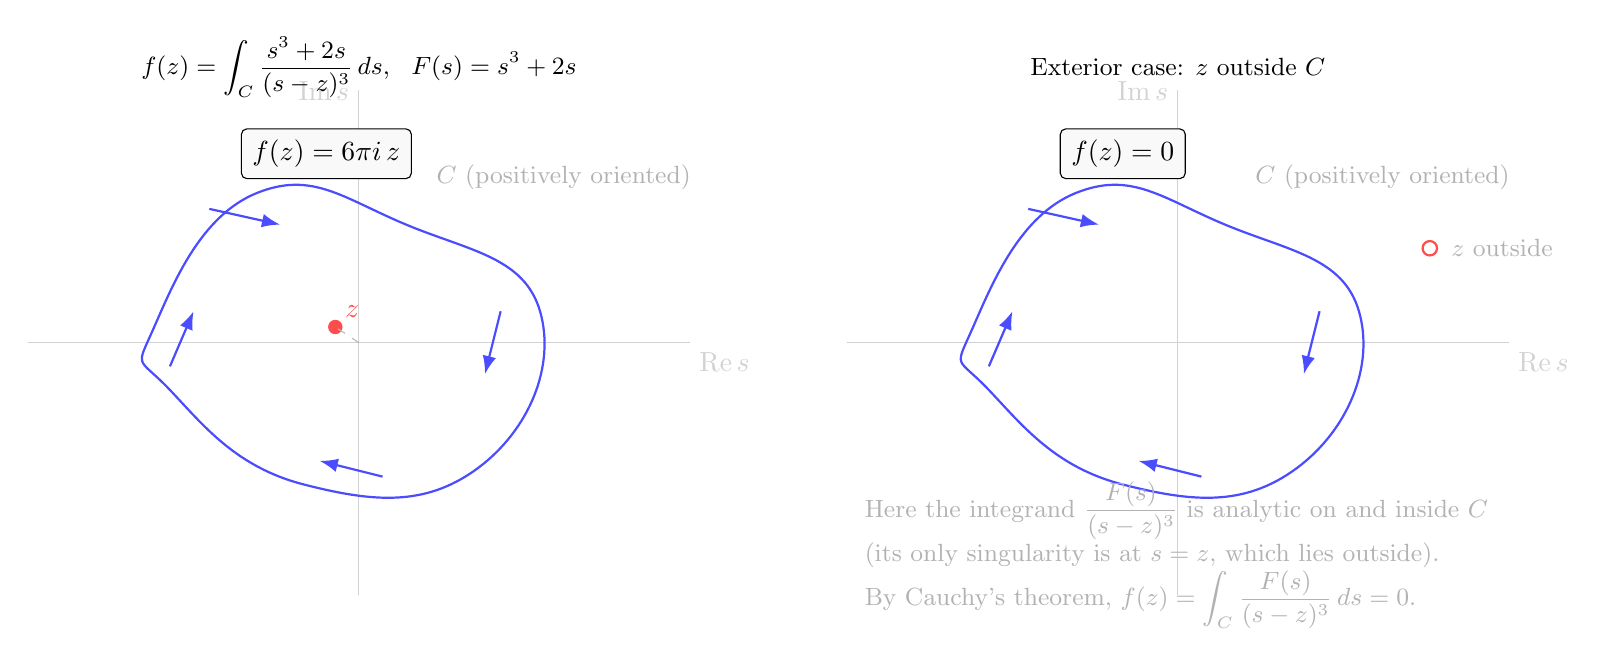
\begin{tikzpicture}[>=Latex,scale=1]
		\tikzset{
			axis/.style={gray!35, line cap=round},
			Ccurve/.style={blue!70, thick},
			orient/.style={-{Latex}, blue!70, thick},
			zin/.style={red!70, fill=red!70},
			zout/.style={red!70, draw=red!70, fill=white, thick},
			note/.style={gray!60, font=\small},
			title/.style={font=\small},
			box/.style={draw, rounded corners=2pt, inner sep=4pt, fill=gray!5}
		}
		
		% =============== LEFT: z inside C =================
		\begin{scope}
			% axes
			\draw[axis] (-4.2,0)--(4.2,0) node[below right] {$\Re s$};
			\draw[axis] (0,-3.2)--(0,3.2) node[left] {$\Im s$};
			\node[title] at (0,3.5)
			{$f(z)=\displaystyle\int_C \frac{s^3+2s}{(s-z)^3}\,ds,\ \ F(s)=s^3+2s$};
			
			% a generic positively oriented simple closed contour C
			\draw[Ccurve] plot[smooth cycle, tension=0.8]
			coordinates{(-2.6,0.2) (-1.3,1.9) (0.6,1.5) (2.3,0.4) (1.5,-1.6) (-0.7,-1.8) (-2.4,-0.6)};
			% orientation arrows along C
%			\foreach \t/\a in {0/20, 0.25/70, 0.5/140, 0.75/220}{
%				\path plot[smooth, tension=0.8, domain=0:1, samples=200] 
%				({-2.6*(1-\x)^6 + ...}); % placeholder
%			}
			% simpler: put four small arrows approximately along the curve
			\draw[orient] (-1.9,1.7) -- ++(0.9,-0.2);
			\draw[orient] ( 1.8,0.4)  -- ++(-0.2,-0.8);
			\draw[orient] ( 0.3,-1.7) -- ++(-0.8,0.2);
			\draw[orient] (-2.4,-0.3) -- ++(0.3,0.7);
			\node[note] at (2.6,2.1) {$C$ (positively oriented)};
			
			% z inside
			\fill[zin] (-0.3,0.2) circle (2.6pt) node[above right] {$z$};
			% indicate triple pole in s at s=z (inside)
			\draw[gray!55,dashed] (0,0) -- (-0.3,0.2);
%			\node[note,anchor=west] at (-4.1,-2.7)
%			{Inside case: pole at $s=z$ of order $3$ is inside $C$.\\
%				Generalized Cauchy (with $n=2$): 
%				$\displaystyle \int_C \frac{F(s)}{(s-z)^3}\,ds=\frac{2\pi i}{2!}F''(z)$.\\
%				Here $F'(s)=3s^2+2,\ F''(s)=6s \Rightarrow f(z)=6\pi i\,z$.};
			
			% small result box
			\node[box,anchor=west] at (-1.5,2.4) {$\displaystyle f(z)=6\pi i\,z$};
		\end{scope}
		
		% =============== RIGHT: z outside C =================
		\begin{scope}[xshift=10.4cm]
			% axes
			\draw[axis] (-4.2,0)--(4.2,0) node[below right] {$\Re s$};
			\draw[axis] (0,-3.2)--(0,3.2) node[left] {$\Im s$};
			\node[title] at (0,3.5) {Exterior case: $z$ outside $C$};
			
			% same contour shape
			\draw[Ccurve] plot[smooth cycle, tension=0.8]
			coordinates{(-2.6,0.2) (-1.3,1.9) (0.6,1.5) (2.3,0.4) (1.5,-1.6) (-0.7,-1.8) (-2.4,-0.6)};
			\draw[orient] (-1.9,1.7) -- ++(0.9,-0.2);
			\draw[orient] ( 1.8,0.4)  -- ++(-0.2,-0.8);
			\draw[orient] ( 0.3,-1.7) -- ++(-0.8,0.2);
			\draw[orient] (-2.4,-0.3) -- ++(0.3,0.7);
			\node[note] at (2.6,2.1) {$C$ (positively oriented)};
			
			% z outside
			\draw[zout] (3.2,1.2) circle (2.6pt);
			\node[note,anchor=west] at (3.35,1.2) {$z$ outside};
			
			% conclusion
			\node[note,align=left,anchor=west] at (-4.1,-2.7)
			{Here the integrand $\dfrac{F(s)}{(s-z)^3}$ is analytic on and inside $C$\\
				(its only singularity is at $s=z$, which lies outside).\\
				By Cauchy’s theorem, $\displaystyle f(z)=\int_C \frac{F(s)}{(s-z)^3}\,ds=0$.};
			
			% small result box
			\node[box,anchor=west] at (-1.5,2.4) {$\displaystyle f(z)=0$};
		\end{scope}		
	\end{tikzpicture}
	\end{center}
\end{proof}
\newpage
\item Let $C$ be the unit circle $z=e^{i\theta}$, $-\pi\le\theta\le\pi$. Show that for any constant $a$,
\[
\int_C \frac{e^{az}}{z}\,dz = 2\pi i.
\] Then writethis integral in term of $\theta$ to derive the integration formula \[
\int_0^\pi e^{a\cos\theta} \cos(a\sin\theta)\,d\theta = \pi.
\]
\begin{proof}[\sol]
	Let $C$ be the unit circle oriented positively. The integrand
	\[
	\frac{e^{a z}}{z}
	\]
	has a simple pole at $z=0$ with residue $\Res_{z=0}\frac{e^{a z}}{z}=e^{a\cdot 0}=1$. By the residue theorem,
	\[
	\int_C \frac{e^{a z}}{z}\,dz \;=\; 2\pi i.
	\]
	
	Now parametrize $C$ by $z=e^{i\theta}$, $-\pi\le \theta\le \pi$. Then $dz=i e^{i\theta}\,d\theta$ and
	\[
	\int_C \frac{e^{a z}}{z}\,dz
	=\int_{-\pi}^{\pi} \frac{e^{a e^{i\theta}}}{e^{i\theta}}\, i e^{i\theta}\,d\theta
	=i\int_{-\pi}^{\pi} e^{a(\cos\theta+i\sin\theta)}\,d\theta
	=i\int_{-\pi}^{\pi} e^{a\cos\theta}\bigl(\cos(a\sin\theta)+i\sin(a\sin\theta)\bigr)\,d\theta.
	\]
	Equating real and imaginary parts with $2\pi i$ gives
	\[
	\int_{-\pi}^{\pi} e^{a\cos\theta}\sin(a\sin\theta)\,d\theta=0,
	\qquad
	\int_{-\pi}^{\pi} e^{a\cos\theta}\cos(a\sin\theta)\,d\theta=2\pi.
	\]
	Since the integrand $e^{a\cos\theta}\cos(a\sin\theta)$ is even in $\theta$, we obtain
	\[
	\int_{0}^{\pi} e^{a\cos\theta}\cos(a\sin\theta)\,d\theta=\pi.
	\]
	\begin{center}
	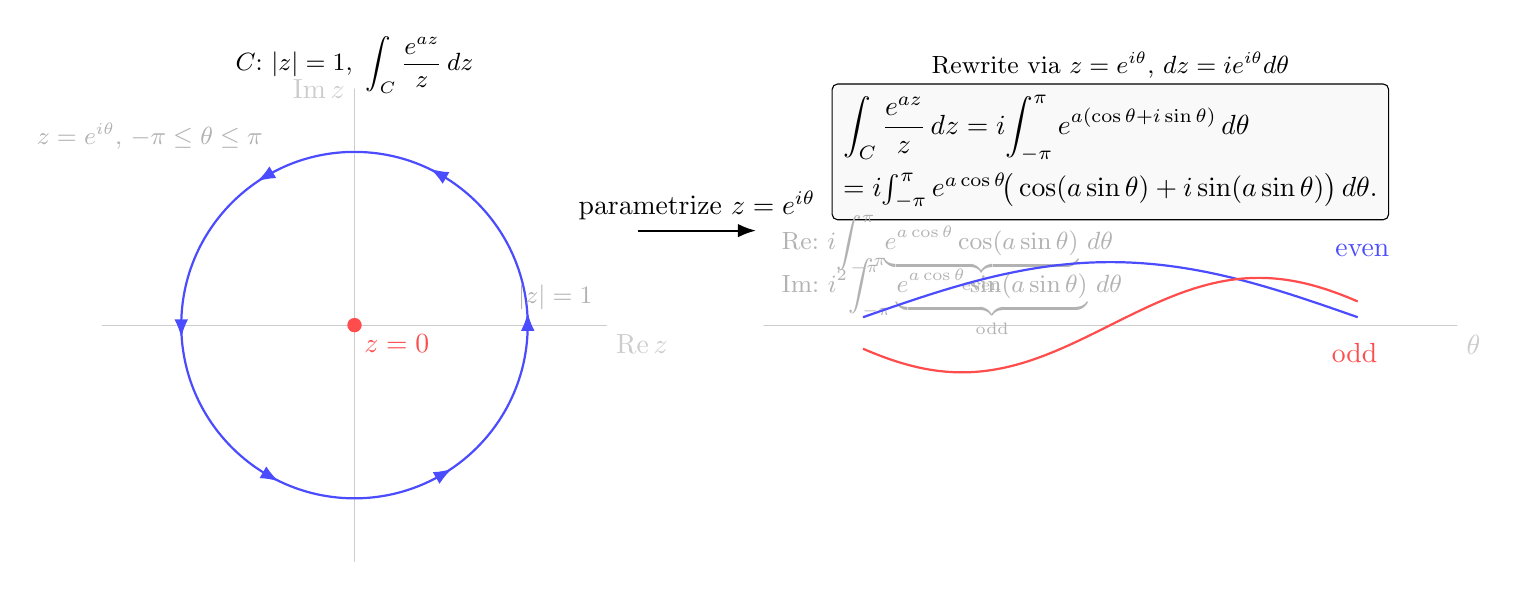
\begin{tikzpicture}[>=Latex,scale=1]
		\tikzset{
			axis/.style={gray!40, line cap=round},
			circ/.style={blue!70, thick},
			orient/.style={-{Latex}, blue!70, thick},
			pole/.style={red!70, fill=red!70},
			note/.style={gray!60, font=\small},
			title/.style={font=\small},
			box/.style={draw, rounded corners=2pt, inner sep=4pt, fill=gray!5}
		}
		
		% ================= LEFT: Complex z-plane, unit circle =================
		\begin{scope}
			% axes
			\draw[axis] (-3.2,0) -- (3.2,0) node[below right] {$\Re z$};
			\draw[axis] (0,-3.0) -- (0,3.0) node[left] {$\Im z$};
			\node[title] at (0,3.3) {$C$:$\ |z|=1,\ \displaystyle \int_C \frac{e^{az}}{z}\,dz$};
			
			% unit circle with CCW orientation
			\draw[circ] (0,0) circle (2.2);
			\foreach \a in {0,60,120,180,240,300}{
				\draw[orient] ({2.2*cos(\a)},{2.2*sin(\a)}) --
				++({0.16*(-sin(\a))},{0.16*(cos(\a))});
			}
			\node[note] at (2.55,0.35) {$|z|=1$};
			
			% pole at z=0, residue 1
			\fill[pole] (0,0) circle (2.6pt) node[below right] {$z=0$};
%			\node[note,anchor=west] at (-3.1,-2.5)
%			{Simple pole at $z=0$, $\Res_{z=0}\!\dfrac{e^{az}}{z}=1$\\[2pt]
%				$\Rightarrow\ \displaystyle \int_C \frac{e^{az}}{z}\,dz=2\pi i$};
			
			% parametrization tag
			\node[note] at (-2.6,2.4) {$z=e^{i\theta}$,\ $-\pi\le\theta\le\pi$};
		\end{scope}
		
		% ============== Arrow between panels ==============
		\draw[-{Latex}, thick] (3.6,1.2) -- (5.1,1.2)
		node[midway,above] {parametrize $z=e^{i\theta}$};
		
		% ================= RIGHT: θ–integral & parity =================
		\begin{scope}[xshift=9.6cm]
			% axes for θ
			\draw[axis] (-4.4,0) -- (4.4,0) node[below right] {$\theta$};
			\node[title] at (0,3.3) {Rewrite via $z=e^{i\theta}$, $dz=i e^{i\theta} d\theta$};
			
			% formula box
			\node[box,align=left] at (0,2.2)
			{$\displaystyle \int_C \frac{e^{az}}{z}\,dz
				= i\!\int_{-\pi}^{\pi} e^{a(\cos\theta+i\sin\theta)}\,d\theta$\\[3pt]
				$= i\!\int_{-\pi}^{\pi} e^{a\cos\theta}\!
				\big(\cos(a\sin\theta)+i\sin(a\sin\theta)\big)\,d\theta.$};
			
			% split into real/imag with parity
			\node[note,anchor=west] at (-4.3,0.9)
			{$\Re$:$\displaystyle\ i\!\int_{-\pi}^{\pi} \underbrace{e^{a\cos\theta}\cos(a\sin\theta)}_{\text{even}}\,d\theta$};
			\node[note,anchor=west] at (-4.3,0.35)
			{$\Im$:$\displaystyle\ i^2\!\int_{-\pi}^{\pi} \underbrace{e^{a\cos\theta}\sin(a\sin\theta)}_{\text{odd}}\,d\theta$};
			
			% even/odd schematic curves
			\draw[blue!70,thick,domain=-3.1416:3.1416,samples=100,smooth]
			plot(\x,{0.7*cos(deg(\x/2)) + 0.1}); % even schematic
			\node[blue!70] at (3.2,0.95) {even};
			\draw[red!70,thick,domain=-3.1416:3.1416,samples=100,smooth]
			plot(\x,{0.6*sin(deg(\x/1.2))}); % odd schematic
			\node[red!70] at (3.1,-0.35) {odd};
			
%			% conclusions
%			\node[note,align=left] at (0,-1.1)
%			{$\displaystyle \int_{-\pi}^{\pi} e^{a\cos\theta}\sin(a\sin\theta)\,d\theta=0$ (odd).\\[4pt]
%				$\displaystyle i\!\int_{-\pi}^{\pi} e^{a\cos\theta}\cos(a\sin\theta)\,d\theta=2\pi i
%				\ \Rightarrow\ 
%				\int_{-\pi}^{\pi} e^{a\cos\theta}\cos(a\sin\theta)\,d\theta=2\pi.$};
%			
%			% final even reduction to [0,π]
%			\node[box,align=left] at (0,-2.5)
%			{$\text{Even integrand}\ \Rightarrow\
%				\displaystyle \int_{0}^{\pi} e^{a\cos\theta}\cos(a\sin\theta)\,d\theta=\pi.$};
		\end{scope}
		
	\end{tikzpicture}
	\end{center}
\end{proof}
\end{enumerate}

%\vspace{1em}
%\noindent Source: lecture note \emph{Complex Variables and Applications, Chapter 4: Integrals (Part II)}. :contentReference[oaicite:0]{index=0}

\newpage
\section{Series}

\subsection{Convergence of Sequences}

\begin{definition}[Limit of a sequence]
	A sequence $(z_n)$ of complex numbers converges to $z\in\C$ if for each $\varepsilon>0$ there exists $N\in\mathbb{N}$ such that
	\[
	|z_n-z|<\varepsilon\qquad(n>N).
	\]
	We write $\lim_{n\to\infty} z_n=z$. If no such $z$ exists, the sequence \emph{diverges}.
\end{definition}

\begin{remark}[Uniqueness]
	A complex sequence has at most one limit.
\end{remark}

\begin{theorem}[Componentwise convergence]
	Let $z_n=x_n+i y_n$ and $z=x+iy$. Then
	\[
	\lim_{n\to\infty} z_n=z
	\quad\Longleftrightarrow\quad
	\lim_{n\to\infty} x_n=x\ \ \text{and}\ \ \lim_{n\to\infty} y_n=y.
	\]
\end{theorem}

\begin{example}
	(a) $z_n=\dfrac{1}{n^3}+i \ \Rightarrow\ \lim z_n=i$. \quad
	(b) $z_n=-2+i\dfrac{(-1)^n}{n^2}\ \Rightarrow\ \lim z_n=-2$.
\end{example}

\begin{observation}[Polar view]
	Writing $z_n=r_n e^{i\theta_n}$ with $r_n=|z_n|$ and $\theta_n=\Arg z_n$, one may have $r_n\to r$ while $(\theta_n)$ fails to converge (e.g.\ even/odd subsequences approaching $\pm\pi$).
\end{observation}

\newpage
\subsection{Convergence of Series}
\defbox[Series and sum]{
	\begin{definition}
		A series $\sum_{n=1}^{\infty} z_n$ converges to $S$ if the partial sums $S_N=\sum_{n=1}^{N} z_n$ satisfy $S_N\to S$. Then $\sum_{n=1}^\infty z_n=S$.
\end{definition}}

\thmbox[Componentwise]{
	\begin{theorem}
		If $z_n=x_n+i y_n$ and $S=X+iY$, then \[
		\sum_{n=1}^{\infty} z_n=S
		\quad\Longleftrightarrow\quad
		\sum_{n=1}^{\infty} x_n=X\ \ \text{and}\ \ \sum_{n=1}^{\infty} y_n=Y.
		\]
\end{theorem}}

\begin{remark}[Necessary test and boundedness]
	If $\sum z_n$ converges, then $z_n\to0$ (the $n$th-term test). In particular, the terms are bounded: there exists $M$ with $|z_n|\le M$ for all $n$.
\end{remark}

\begin{definition}[Absolute convergence]
	$\sum z_n$ is \emph{absolutely convergent} if $\sum |z_n|$ converges. Absolute convergence implies convergence.
\end{definition}

\begin{remark}[Remainders]
	If $S=\sum_{n=1}^\infty z_n$, the remainder after $N$ terms is $\rho_N=S-S_N$. Then $S_N\to S$ iff $\rho_N\to 0$.
\end{remark}

\subsection{Power Series and Taylor Series}
\defbox[Power series centered at $z_0$]{
	\begin{definition}
		\[
		\sum_{n=0}^{\infty} a_n (z-z_0)^n=a_0+a_1(z-z_0)+a_2(z-z_0)^2+\cdots,
		\]
		with $a_n,z_0\in\C$.
\end{definition}}

\thmbox[Taylor series]{
	\begin{theorem}\label{thm:Taylor}
		If $f$ is analytic on $|z-z_0|<R_0$, then for $|z-z_0|<R_0$,
		\[
		f(z)=\sum_{n=0}^{\infty} a_n (z-z_0)^n,\qquad a_n=\frac{f^{(n)}(z_0)}{n!}.
		\]
		For $z_0=0$ this is the \emph{Maclaurin series}.
\end{theorem}}

\begin{example}
	Since $e^z$ is entire,
	\[
	e^z=\sum_{n=0}^{\infty}\frac{z^n}{n!},\qquad
	z^2 e^{3z}=\sum_{n=0}^{\infty}\frac{3^{\,n-2}}{(n-2)!}\,z^{n}\quad(\text{interpreting }(n-2)!=\infty \text{ for }n<2\text{ gives zero terms}).
	\]
	Also
	\[
	\sin z=\sum_{n=0}^{\infty}\frac{(-1)^n z^{2n+1}}{(2n+1)!},\quad
	\cos z=\sum_{n=0}^{\infty}\frac{(-1)^n z^{2n}}{(2n)!},
	\]
	\[
	\sinh z=\sum_{n=0}^{\infty}\frac{z^{2n+1}}{(2n+1)!},\quad
	\cosh z=\sum_{n=0}^{\infty}\frac{z^{2n}}{(2n)!}.
	\]
\end{example}

\begin{example}[Geometric series]
	For $f(z)=\dfrac{1}{1-z}$ we have
	\[
	\frac{1}{1-z}=\sum_{n=0}^{\infty} z^n,\qquad |z|<1,
	\]
	and similarly $\dfrac{1}{1+z}=\sum_{n=0}^{\infty}(-1)^n z^n$ for $|z|<1$.
\end{example}

\subsection{Laurent Series}

\begin{remark}
	At a point $z_0$ where $f$ is not analytic, Taylor series may fail; on an annulus $R_1<|z-z_0|<R_2$ one often has a two-sided power expansion (Laurent series).
\end{remark}

\begin{theorem}[Laurent]\label{thm:Laurent}
	If $f$ is analytic on the annulus $R_1<|z-z_0|<R_2$ and $C$ is any positively oriented simple closed contour around $z_0$ lying in that annulus, then on $R_1<|z-z_0|<R_2$,
	\[
	f(z)=\sum_{n=0}^{\infty} a_n (z-z_0)^n+\sum_{n=1}^{\infty} \frac{b_n}{(z-z_0)^n}
	=\sum_{n=-\infty}^{\infty} c_n (z-z_0)^n,
	\]
	with
	\[
	c_n=\frac{1}{2\pi i}\int_C \frac{f(\zeta)}{(\zeta-z_0)^{n+1}}\,d\zeta\qquad (n\in\mathbb{Z}).
	\]
	If $f$ is analytic on $|z-z_0|<R_2$ then $b_n=0$ and Laurent reduces to Taylor.
\end{theorem}

\begin{example}
	Since $e^z=\sum_{n=0}^\infty \dfrac{z^n}{n!}$ for all $z$, we get
	\[
	e^{1/z}=\sum_{n=0}^{\infty}\frac{1}{n!}\,\frac{1}{z^n},\qquad 0<|z|<\infty.
	\]
	The coefficient of $(z^{-1})$ is $1$, hence for any positively oriented simple closed contour $C$ around $0$,
	\[
	\int_C e^{1/z}\,dz = 2\pi i.
	\]
\end{example}

\begin{example}[Partial fractions across annuli]
	Let
	\[
	f(z)=\frac{-1}{(z-1)(z-2)}=\frac{1}{z-1}-\frac{1}{z-2}.
	\]
	Three Laurent expansions in powers of $z$ arise:
	\begin{align*}
		|z|<1:&\quad f(z)= -\sum_{n=0}^{\infty} z^{n}+\sum_{n=0}^{\infty}\frac{z^{n}}{2^{\,n+1}}
		= \sum_{n=0}^{\infty}\Big(\frac{1}{2^{\,n+1}}-1\Big) z^{n},\\[2pt]
		1<|z|<2:&\quad f(z)= \sum_{n=0}^{\infty}\frac{1}{z^{n+1}}+\sum_{n=0}^{\infty}\frac{z^{n}}{2^{\,n+1}}
		= \sum_{n=1}^{\infty}\frac{1}{z^{n}}+\sum_{n=0}^{\infty}\frac{z^{n}}{2^{\,n+1}},\\[2pt]
		|z|>2:&\quad f(z)= \sum_{n=1}^{\infty}\frac{1-2^{\,n-1}}{z^{n}}.
	\end{align*}
\end{example}

%\begin{example}
%	Find the Laurent series
%\end{example}

\subsection{Absolute and Uniform Convergence of Power Series}

\begin{theorem}[Absolute convergence inside any interior circle]
	If a power series $\sum_{n=0}^{\infty} a_n (z-z_0)^n$ converges at some $z_1\ne z_0$, then it converges absolutely for all $|z-z_0|<|z_1-z_0|$.
\end{theorem}

\begin{definition}[Circle of convergence]
	The largest open disk centered at $z_0$ on which the series converges is the \emph{circle of convergence}. Its radius is the \emph{radius of convergence}.
\end{definition}

\begin{theorem}[Uniform convergence on closed interior disks]
	If $|z_1-z_0|=R_1$ lies strictly inside the circle $|z-z_0|=R$, then the series is uniformly convergent on the closed disk $|z-z_0|\le R_1$.
\end{theorem}

\subsection{Consequences for Sums of Power/Laurent Series}
$\wedge$
\begin{theorem}[Continuity and analyticity]\label{thm:cont-anal}
	Inside the circle of convergence, the sum $S(z)=\sum_{n=0}^{\infty} a_n (z-z_0)^n$ is continuous and analytic.
\end{theorem}

\begin{remark}[Exterior series]
	If $\sum_{n=1}^{\infty} \dfrac{b_n}{(z-z_0)^n}$ converges at $z_1\ne z_0$, then it converges absolutely to a continuous function on $\{|z-z_0|>|z_1-z_0|\}$ (the exterior of the circle through $z_1$).
\end{remark}

\begin{remark}[Laurent on annuli]
	If
	\[
	f(z)=\sum_{n=0}^{\infty} a_n (z-z_0)^n+\sum_{n=1}^{\infty}\frac{b_n}{(z-z_0)^n}
	\]
	is valid on $R_1<|z-z_0|<R_2$, then both series converge uniformly on any closed annulus $R_1+\varepsilon \le |z-z_0|\le R_2-\varepsilon$ ($\varepsilon>0$).
\end{remark}

\begin{theorem}[Termwise integration on interior contours]
	Let $C$ be a contour inside the circle of convergence of $\sum_{n=0}^{\infty} a_n (z-z_0)^n$ and $f$ continuous on $C$. Then
	\[
	\int_C f(z)\,\sum_{n=0}^{\infty} a_n (z-z_0)^n\,dz
	=\sum_{n=0}^{\infty} a_n \int_C f(z)(z-z_0)^n\,dz.
	\]
\end{theorem}

\begin{corollary}
	The sum $S(z)$ is analytic inside its circle of convergence and may be integrated term by term on interior contours.
\end{corollary}

\begin{example}
	Define
	\[
	f(z)=
	\begin{cases}
		\dfrac{e^{z}-1}{z},& z\ne 0,\\[4pt]
		1,& z=0.
	\end{cases}
	\]
	Since $e^{z}-1=\sum_{n=1}^\infty \dfrac{z^{n}}{n!}$, we obtain $f(z)=\sum_{n=1}^\infty \dfrac{z^{n-1}}{n!}$ for all $z$ with the limit at $0$ equal to $1$. Thus $f$ is entire and continuous at $0$.
\end{example}

\begin{theorem}[Termwise differentiation]
	Inside the circle of convergence,
	\[
	\frac{d}{dz}\sum_{n=0}^{\infty} a_n (z-z_0)^n
	= \sum_{n=1}^{\infty} n a_n (z-z_0)^{n-1}.
	\]
\end{theorem}

\begin{theorem}[Uniqueness of Taylor/Laurent expansions]
	If a power series in $(z-z_0)$ equals $f(z)$ on a disk, it is the Taylor series of $f$. If a doubly-infinite series $\sum_{n=-\infty}^{\infty} c_n (z-z_0)^n$ equals $f$ on an annulus, it is the Laurent expansion of $f$ on that annulus.
\end{theorem}

\begin{corollary}[Cauchy product]
	If
	\[
	f(z)=\sum_{n=0}^{\infty} a_n (z-z_0)^n,\qquad
	g(z)=\sum_{n=0}^{\infty} b_n (z-z_0)^n
	\]
	converge on $|z-z_0|<R$, then
	\[
	f(z)g(z)=\sum_{n=0}^{\infty}\Bigg(\sum_{k=0}^{n} a_k b_{n-k}\Bigg)(z-z_0)^n,\qquad |z-z_0|<R.
	\]
\end{corollary}


\newpage
\subsection{Exercises}
\begin{enumerate}[\bf 1.]
	\item Show that the limit of a convergent complex sequence is unique by appealing to the corresponding result for a sequence of real numbers.
	\begin{proof}[\sol]
		We want to show that \begin{center}
		``If a complex sequence $\set{z_n}$ converges to both $L$ and $M$ in $\mathbb{C}$, then $L=M$.''
		\end{center}
		Write $z_n=x_n+iy_n$, $L=a+ib$, $M=c+id$ with $x_n,y_n,a,b,c,d\in\mathbb{R}$.
		Assume that \[
		z_n\to L\quad\text{and}\quad z_n\to M
		\] as $n\to\infty$. Taking real and imaginary parts, \[
		x_n=\Re z_n \to \Re L=a \quad\text{and}\quad x_n=\Re z_n \to \Re M=c,
		\] \[
		y_n=\Im z_n \to \Im L=b \quad\text{and}\quad y_n=\Im z_n \to \Im M=d.
		\]
		By the \emph{uniqueness of limits for real sequences}, these imply $a=c$ and $b=d$. Hence \[
		L=a+ib=c+id=M.
		\]
%		\begin{center}
%		\begin{tikzpicture}[>=Latex,scale=1]
%			\tikzset{
%				axis/.style={gray!40, line cap=round},
%				pt/.style={black, fill=red},
%				seq/.style={blue!70, fill=blue!70},
%				ballL/.style={draw=green!60!black, fill=green!20},
%				ballM/.style={draw=red!70!black,   fill=red!15},
%				note/.style={gray!60, font=\small},
%				title/.style={font=\small}
%			}
%			% ================= LEFT: ε-balls argument =================
%			\begin{scope}
%				% axes
%				\draw[axis] (-3.2,0) -- (3.2,0) node[below right] {$\Re z$};
%				\draw[axis] (0,-2.6) -- (0,2.6) node[left] {$\Im z$};
%				\node[title] at (0,2.9) {Uniqueness via disjoint $\varepsilon$-balls};
%				
%				% candidate limits
%				\coordinate (L) at (-1.0,0.6);
%				\coordinate (M) at ( 1.1,-0.2);
%				
%				% pick radii (schematic: half the distance)
%				\def\rL{0.9}
%				\def\rM{0.9}
%				
%				% balls and points
%				\draw[ballL] (L) circle (\rL);
%				\draw[ballM] (M) circle (\rM);
%				\fill[pt] (L) circle (2pt) node[above left] {$L$};
%				\fill[pt] (M) circle (2pt) node[below right] {$M$};
%				
%				% sample tail points near L
%				\fill[seq] ($(L)+(-0.25, 0.10)$) circle (1.8pt);
%				\fill[seq] ($(L)+(-0.10, 0.00)$) circle (1.8pt);
%				\fill[seq] ($(L)+(-0.05,-0.08)$) circle (1.8pt);
%				
%				% sample tail points near M
%				\fill[seq] ($(M)+( 0.20,-0.05)$) circle (1.8pt);
%				\fill[seq] ($(M)+( 0.05, 0.07)$) circle (1.8pt);
%				\fill[seq] ($(M)+(-0.10, 0.00)$) circle (1.8pt);
%				
%				\node[note,align=left] at (0.0,2.0)
%				{If $L\neq M$, take $\varepsilon=\tfrac12|L-M|$ so
%					$B(L,\varepsilon)\cap B(M,\varepsilon)=\varnothing$.\\
%					Since $z_n\to L$ and $z_n\to M$, the tail must lie in both balls — impossible.};
%			\end{scope}
%			% ================= RIGHT: component-wise argument =================
%			\begin{scope}[xshift=9.0cm]
%				\node[title] at (0,2.9) {Component-wise: real limits are unique};
%				
%				% real axis (top) and imaginary axis (bottom)
%				\draw[axis] (-3.2, 1.5) -- (3.2, 1.5) node[below right] {$\Re$};
%				\draw[axis] (-3.2,-1.5) -- (3.2,-1.5) node[below right] {$\Im$};
%				
%				% real parts: a = Re L, c = Re M
%				\coordinate (a) at (-0.6, 1.5);
%				\coordinate (c) at ( 0.6, 1.5);
%				\fill[pt] (a) circle (2pt) node[above] {$a=\Re L$};
%				\fill[pt] (c) circle (2pt) node[above] {$c=\Re M$};
%				
%				% imaginary parts: b = Im L, d = Im M
%				\coordinate (b) at (-0.4,-1.5);
%				\coordinate (d) at ( 0.9,-1.5);
%				\fill[pt] (b) circle (2pt) node[below] {$b=\Im L$};
%				\fill[pt] (d) circle (2pt) node[below] {$d=\Im M$};
%				
%				% schematic tails for x_n and y_n
%				\foreach \x in {-1.6,-1.2,-0.9,-0.75,-0.65} {
%					\fill[seq] (\x,1.5) circle (1.5pt);
%				}
%				\foreach \x in {1.6,1.2,0.9,0.75,0.65} {
%					\fill[seq] (\x,1.5) circle (1.5pt);
%				}
%				\foreach \y in {-1.7,-1.3,-1.0,-0.7,-0.5} {
%					\fill[seq] (\y,-1.5) circle (1.5pt);
%				}
%				\foreach \y in {1.7,1.3,1.0,0.7,0.5} {
%					\fill[seq] (\y,-1.5) circle (1.5pt);
%				}
%				
%				% notes
%				\node[note,align=left] at (0,0.5)
%				{$x_n=\Re z_n\to a\ \text{and}\ x_n\to c\ \Rightarrow\ a=c$ (uniqueness in $\mathbb R$).};
%				\node[note,align=left] at (0,-0.1)
%				{$y_n=\Im z_n\to b\ \text{and}\ y_n\to d\ \Rightarrow\ b=d$ (uniqueness in $\mathbb R$).};
%				
%				% conclusion
%				\node[note,draw,rounded corners=2pt,fill=gray!5] at (0,-2.3)
%				{$a=c,\ b=d \ \Rightarrow\ L=a+ib=c+id=M$.};
%			\end{scope}
%		\end{tikzpicture}
%		\end{center}
	\end{proof}
	\item Show that \[
	\sum_{n=1}^{\infty} z_n=S\implies \sum_{n=1}^{\infty} \overline{z_n}=\overline{S}.
	\]
	\begin{proof}[\sol]
		Let $s_N:=\sum_{n=1}^{N} z_n$ be the partial sums. By hypothesis $s_N\to S$ as $N\to\infty$.
		Consider the conjugated partial sums
		\[
		\overline{s_N}=\overline{\sum_{n=1}^{N} z_n}=\sum_{n=1}^{N}\overline{z_n},
		\]
		so $\{\overline{s_N}\}$ are the partial sums of $\sum_{n=1}^{\infty}\overline{z_n}$.
		Since complex conjugation is continuous (indeed, an isometry: $|\overline{w}-\overline{z}|=|w-z|$),
		we have $\overline{s_N}\to\overline{S}$. Therefore the series $\sum_{n=1}^{\infty}\overline{z_n}$ converges and
		\[
		\sum_{n=1}^{\infty}\overline{z_n}=\lim_{N\to\infty}\sum_{n=1}^{N}\overline{z_n}
		=\lim_{N\to\infty}\overline{s_N}=\overline{S}.
		\]
	\end{proof}
	\item Derive the Taylor series representation \[
	\frac{1}{1-z}=\sum_{n=0}^{\infty}\frac{(z-i)^n}{(1-i)^{\,n+1}},\qquad |z-i|<\sqrt{2}.
	\] 
	\begin{proof}[\sol]
	Note that \[
	\frac{1}{1-z}
	=\frac{1}{(1-i)-(z-i)}
	=\frac{1}{1-i}\cdot\frac{1}{1-\left(\frac{z-i}{1-i}\right)}.
	\] For \(\left|\dfrac{z-i}{1-i}\right|<1\) (i.e. \(|z-i|<|1-i|=\sqrt{2}\)), expand the geometric series:
	\[
	\frac{1}{1-w}=\sum_{n=0}^{\infty} w^{n}\quad (|w|<1),\qquad
	w=\frac{z-i}{1-i}.
	\] Hence \[
	\frac{1}{1-z}
	=\frac{1}{1-i}\sum_{n=0}^{\infty}\left(\frac{z-i}{1-i}\right)^n
	=\sum_{n=0}^{\infty}\frac{(z-i)^n}{(1-i)^{\,n+1}},
	\]
	which converges for \(|z-i|<\sqrt{2}\).
	\begin{center}
	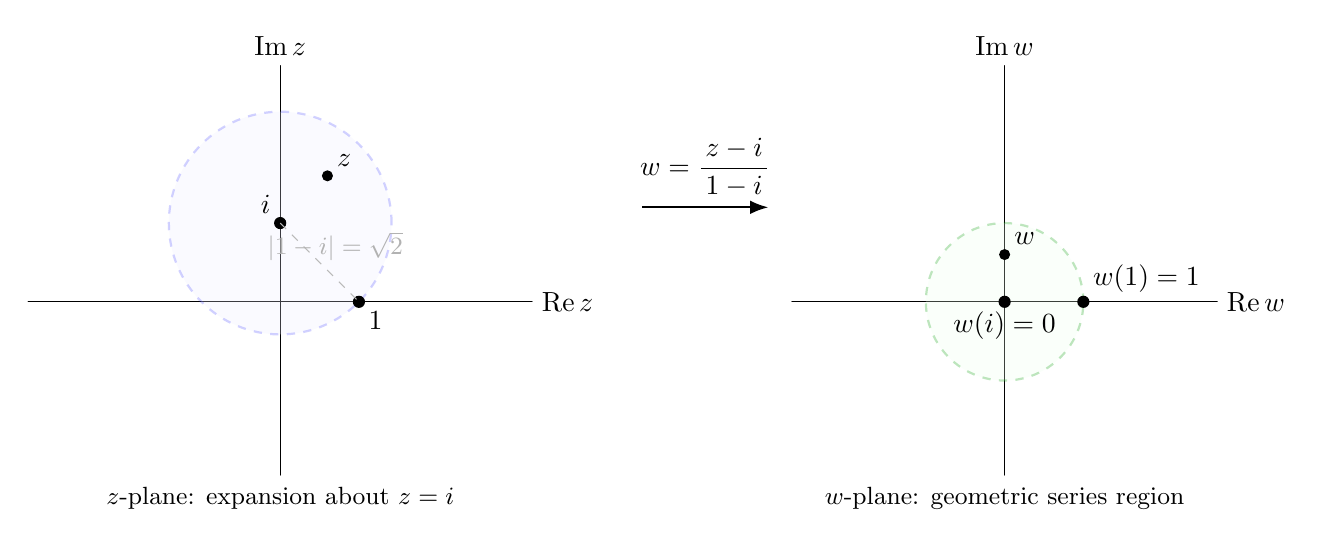
\begin{tikzpicture}[>=Latex,scale=1]
		\tikzset{
			axis/.style={black, line cap=round},
			disk/.style={draw=blue!70, fill=blue!8, thick, opacity=.25, dashed},
			unit/.style={draw=green!60!black, fill=green!8, thick, opacity=.25, dashed},
			note/.style={gray!60, font=\small},
			title/.style={font=\small},
			point/.style={black, fill=black},
			maparrow/.style={-{Latex}, thick}
		}
		% ================= LEFT: z-plane =================
		\begin{scope}
			% axes
			\draw[axis] (-3.2,0) -- (3.2,0) node[right] {$\Re z$};
			\draw[axis] (0,-2.2) -- (0,3.0) node[above] {$\Im z$};
			\node[title] at (0,-2.5) {$z$-plane: expansion about $z=i$};
			% disk centered at i with radius sqrt(2)
			\def\R{1.4142}
			\draw[disk] (0,1) circle (\R);
			% key points: i and 1
			\fill[point] (0,1) circle (2.2pt) node[above left] {$i$};
			\fill[point] (1,0) circle (2.2pt) node[below right] {$1$};	
			% show that 1 is on the boundary: |1-i|=sqrt(2)
			\draw[gray!55,dashed] (0,1) -- (1,0);
			\node[note] at (0.7,0.7) {$|1-i|=\sqrt{2}$};	
			% a sample z inside the disk
			\coordinate (Z) at (0.6,1.6);
			\fill (Z) circle (2.0pt) node[above right] {$z$};
		\end{scope}
		% mapping arrow
		\draw[maparrow] (4.6,1.2) -- (6.2,1.2)
		node[midway,above] {$\displaystyle w=\frac{z-i}{\,1-i\,}$};
		
		% ================= RIGHT: w-plane =================
		\begin{scope}[xshift=9.2cm]
			% axes
			\draw[axis] (-2.7,0) -- (2.7,0) node[right] {$\Re w$};
			\draw[axis] (0,-2.2) -- (0,3) node[above] {$\Im w$};
			\node[title] at (0,-2.5) {$w$-plane: geometric series region};
			
			% unit disk |w|<1
			\draw[unit] (0,0) circle (1);
			
			% images of key points: i -> 0, 1 -> 1
			\fill[point] (0,0) circle (2.2pt) node[below] {$w( i)=0$};
			\fill[point] (1,0) circle (2.2pt) node[above right] {$w(1)=1$};
			
			% image of sample z
			% For Z=(0.6,1.6): z-i=(0.6,0.6), 1-i=(1,-1) so w=(0.6+0.6i)/(1-i)=0.6i
			\coordinate (W) at (0,0.6);
			\fill (W) circle (2.0pt) node[above right] {$w$};
			
%			% formula box
%			\node[note,draw,rounded corners=2pt,fill=gray!5,align=left] at (0,-2.0)
%			{$\displaystyle \frac{1}{1-z}
%				=\frac{1}{(1-i)-(z-i)}
%				=\frac{1}{1-i}\cdot\frac{1}{1-\left(\frac{z-i}{1-i}\right)}$\\[4pt]
%				If $|w|=\left|\dfrac{z-i}{1-i}\right|<1$:
%				$\displaystyle\ \frac{1}{1-w}=\sum_{n=0}^\infty w^n$\\[4pt]
%				$\displaystyle \Rightarrow\ \frac{1}{1-z}
%				=\sum_{n=0}^\infty \frac{(z-i)^n}{(1-i)^{\,n+1}},\quad |z-i|<\sqrt{2}.$};
		\end{scope}
	\end{tikzpicture}
	\end{center}
	\end{proof}
	\newpage
	\item Show that the two Laurent series in powers of $z$ that represent the function \[
	f(z)=\frac{1}{z(1+z^2)}
	\] are\[
	\sum_{n=0}^{\infty}(-1)^{n+1} z^{2n+1}+\frac{1}{z}\quad(0<|z|<1),
	\qquad
	\sum_{n=1}^{\infty}\frac{(-1)^{n+1}}{z^{2n+1}}\quad(1<|z|<\infty).
	\]
	\begin{proof}[\sol]
	\begin{enumerate}[(1)]
		\item (\(0<|z|<1\))\quad Since \[
		\frac{1}{1+z^2}=\frac{1}{1-(-z^2)}=\sum_{n=0}^\infty (-z^2)^n=\sum_{n=0}^\infty (-1)^n z^{2n}\qquad(|z|<1),
		\] we have \begin{align*}
			\frac{1}{z(1+z^2)}=\frac{1}{z}\sum_{n=0}^\infty (-1)^n z^{2n}
			&=\sum_{n=0}^\infty (-1)^n z^{2n-1}\\
			&=\frac{1}{z}+\left(-z\right)+z^3+(-z^5)+z^7+\cdots\\
			&=\frac{1}{z}+\sum_{n=0}^\infty (-1)^{n+1} z^{2n+1}.
		\end{align*}
		Therefore the Laurent series on \(0<|z|<1\) is $\displaystyle \sum_{n=0}^{\infty}(-1)^{n+1} z^{2n+1}+\frac{1}{z}$.
		\item (\(1<|z|<\infty\))\quad Since \[
		\frac{1}{1+z^2}=\frac{1}{z^2}\,\frac{1}{1+z^{-2}}=\frac{1}{z^2}\,\frac{1}{1-(-z^{-2})}
		=\frac{1}{z^2}\sum_{n=0}^\infty (-1)^n z^{-2n}\qquad(|z|>1),
		\] we obtain \begin{align*}		
			\frac{1}{z(1+z^2)}=\frac{1}{z}\cdot\frac{1}{z^2}\sum_{n=0}^\infty (-1)^n z^{-2n}
			&=\sum_{n=0}^\infty \frac{(-1)^n}{z^{2n+3}}\\
			&=\frac{1}{z^3}+\frac{-1}{z^5}+\frac{1}{z^7}+\frac{-1}{z^9}+\cdots \\
			&=\sum_{n=1}^\infty \frac{(-1)^{n+1}}{z^{2n+1}},
		\end{align*} Hence the Laurent series is $\displaystyle \sum_{n=1}^{\infty}\frac{(-1)^{n+1}}{z^{2n+1}}$ on \(1<|z|<\infty\).
	\end{enumerate} 
	\end{proof}
	\item Let $a\in\R$, where $-1<a<1$. Then the Laurent series representation $a/(z-a)$ is \[
	\frac{a}{z-a}=\sum_{n=1}^{\infty}\frac{a^{n}}{z^{n}},\qquad |a|<|z|<\infty.
	\]
	After writing $z=e^{i\theta}$ in the above equation, equate real parts and then imaginary parts on each side of the result to derive the summation formulas:
	\[
	\sum_{n=1}^{\infty} a^n \cos(n\theta)=\frac{a\cos\theta-a^2}{1-2a\cos\theta+a^2}\quad\text{and}\quad
	\sum_{n=1}^{\infty} a^n \sin(n\theta)=\frac{a\sin\theta}{1-2a\cos\theta+a^2}.
	\]
	\begin{proof}[\sol]
		For $|a|<|z|$, we know that
		\[
		\frac{a}{z-a}
		=\frac{a}{z}\,\frac{1}{1-a/z}
		=\frac{a}{z}\,\sum_{n=0}^\infty\left(\frac{a}{z}\right)^n
		=\sum_{n=0}^\infty\left(\frac{a}{z}\right)^{n+1}
		=\sum_{n=1}^{\infty}\frac{a^{n}}{z^{n}}.
		\] Set $z=e^{i\theta}$ (so $|a|<|z|=1$). Then
		\[
		\frac{a}{e^{i\theta}-a}=\sum_{n=1}^{\infty} a^n e^{-in\theta}
		=\sum_{n=1}^{\infty} a^n\bigl(\cos(n\theta)-i\sin(n\theta)\bigr).
		\]
		Note that \begin{align*}
			\frac{a}{e^{i\theta}-a}
			=\frac{e^{-i\theta}}{e^{-i\theta}}\cdot\frac{a}{e^{i\theta}-a}
			=\frac{a e^{-i\theta}}{1-a e^{-i\theta}}
			=\frac{a e^{-i\theta}(1-a e^{i\theta})}{(1-a e^{i\theta})(1-a e^{-i\theta})}
			&=\frac{a e^{-i\theta}(1-a e^{i\theta})}{1-a(e^{i\theta}+e^{-i\theta})+a^2e^{i\theta-i\theta}}\\
			&=\frac{a\,(e^{-i\theta}-a)}{1-2a\cos\theta+a^2}\\
			&=\frac{a\,(\cos\theta-i\sin\theta-a)}{1-2a\cos\theta+a^2}\\
			&=\frac{a(\cos\theta-a)-i\,a\sin\theta}{1-2a\cos\theta+a^2}.
		\end{align*} Thus, we obtain \[
		\sum_{n=1}^{\infty} a^n\bigl(\cos(n\theta)-i\sin(n\theta)\bigr)=\frac{a}{e^{i\theta}-a}=\frac{a(\cos\theta-a)-i\,a\sin\theta}{1-2a\cos\theta+a^2}.
		\] Therefore \[
		\boxed{\ \sum_{n=1}^{\infty} a^n \cos(n\theta)=\frac{a\cos\theta-a^2}{1-2a\cos\theta+a^2},\qquad
			\sum_{n=1}^{\infty} a^n \sin(n\theta)=\frac{a\sin\theta}{1-2a\cos\theta+a^2}\ },
		\]
		valid for $-1<a<1$ (indeed $1-2a\cos\theta+a^2=(1-a e^{i\theta})(\overline{1-a e^{i\theta}})=|1-ae^{i\theta}|^2>0$).
	\end{proof}
	\item With the aid of series, show that the function $f$ defined by means of the equations \[
	f(z)=\begin{cases}
		(\sin z)/z &: z\neq 0\\
		1 &: z = 0
	\end{cases}\] is entire. Use this result to establish the limit \[
	\lim_{z\to0}\frac{\sin z}{z}=1.
	\]
	\begin{proof}[\sol]
		The Maclaurin series of $\sin z$ (entire) is
		\[
		\sin z=\sum_{n=0}^{\infty}(-1)^n\frac{z^{2n+1}}{(2n+1)!}\,.
		\]
		For $z\neq 0$, divide by $z$:
		\[
		\frac{\sin z}{z}=\sum_{n=0}^{\infty}(-1)^n\frac{z^{2n}}{(2n+1)!}
		=1-\frac{z^{2}}{3!}+\frac{z^{4}}{5!}-\cdots .
		\]
		This is a power series with infinite radius of convergence, hence defines an entire function
		\[
		F(z):=\sum_{n=0}^{\infty}(-1)^n\frac{z^{2n}}{(2n+1)!}.
		\]
		Note that $F(0)=1$, and for $z\neq 0$ we have $F(z)=\sin z/z$. Therefore $f\equiv F$ on $\mathbb{C}$; in particular, $f$ is entire (the singularity at $0$ is removable). By continuity of $F$ at $0$, \[
		\lim_{z\to 0}\frac{\sin z}{z}=\lim_{z\to 0}F(z)=F(0)=1.
		\]
	\end{proof}
%	\begin{center}
%	\begin{tikzpicture}[>=Latex,scale=1]
%		\tikzset{
%			axis/.style={gray!40, line cap=round},
%			title/.style={font=\small},
%			note/.style={gray!60, font=\small},
%			entire/.style={draw=blue!60, line width=0.9pt},
%			hole/.style={draw=red!70, fill=white, line width=0.9pt},
%			filled/.style={draw=green!60!black, fill=green!60!black},
%			seriesbox/.style={draw, rounded corners=2pt, fill=gray!5, inner sep=4pt}
%		}
%		
%		% ================= LEFT: Complex plane & removable singularity =================
%		\begin{scope}
%			% axes
%			\draw[axis] (-3.4,0)--(3.4,0) node[below right] {$\Re z$};
%			\draw[axis] (0,-3.0)--(0,3.2) node[left] {$\Im z$};
%			\node[title] at (0,3.5) {$F(z)=\sum_{n=0}^{\infty}(-1)^n\dfrac{z^{2n}}{(2n+1)!}$ is entire; $F(0)=1$};
%			
%			% concentric disks to suggest infinite radius (entire)
%			\foreach \R in {0.6,1.2,1.8,2.4,3.0}{
%				\draw[entire] (0,0) circle (\R);
%			}
%			\node[note] at (2.5,2.4) {radius $=\infty$};
%			
%			% removable singularity at 0 for sin z / z (hole) and its filling by F(0)=1
%			\draw[hole] (0,0) circle (2.4pt); % the "hole" of sin z / z at 0
%			\node[note,anchor=west] at (0.15,0.15) {$\dfrac{\sin z}{z}$ undefined at $0$};
%			
%			% same point filled when defining F(0)=1
%			\fill[filled] (0,0) circle (1.7pt);
%			\node[note,anchor=west] at (0.15,-0.2) {$F(0)=1$ (removable)};
%			
%			% series box
%			\node[seriesbox,align=left] at (-2.1,-2.2)
%			{$\displaystyle \sin z=\sum_{n\ge0}(-1)^n\frac{z^{2n+1}}{(2n+1)!}$\\[4pt]
%				For $z\neq0$:\ $\displaystyle \frac{\sin z}{z}=\sum_{n\ge0}(-1)^n\frac{z^{2n}}{(2n+1)!}$\\[4pt]
%				Define $F(0)=1$ $\Rightarrow$ $F$ entire and $F(z)=\dfrac{\sin z}{z}$ for $z\neq0$.};
%		\end{scope}
%		
%		% =============== RIGHT: Real slice y = sin x / x with removable point ===============
%		\begin{scope}[xshift=9.5cm]
%			% axes for real plot
%			\draw[axis] (-5.4,0)--(5.4,0) node[below right] {$x=\Re z$};
%			\draw[axis] (0,-0.5)--(0,1.6) node[left] {$y$};
%			\node[title] at (0,1.9) {Real slice: $y=\dfrac{\sin x}{x}$ and the limit $x\to0$};
%			
%			% plot sin x / x on (-5.2,-0.2] and [0.2,5.2]
%			\draw[blue!70, line width=0.9pt, domain=-5.2:-0.2, samples=200, smooth]
%			plot(\x,{sin(deg(\x))/\x});
%			\draw[blue!70, line width=0.9pt, domain=0.2:5.2, samples=200, smooth]
%			plot(\x,{sin(deg(\x))/\x});
%			
%			% open circle at (0,1) for sin x / x
%			\draw[hole] (0,1) circle (2.4pt);
%			\node[note,anchor=west] at (0.15,1.1) {$\big(\sin x)/x$ undefined at $0$};
%			
%			% filled dot at (0,1) for F(0)=1
%			\fill[filled] (0,1) circle (1.7pt);
%			\node[note,anchor=west] at (0.15,0.8) {$F(0)=1$};
%			
%			% label of limit
%			\node[seriesbox] at (3.2,1.35) {$\displaystyle \lim_{x\to0}\frac{\sin x}{x}=1$};
%		\end{scope}
%	\end{tikzpicture}
%	\end{center}
\end{enumerate}

%\vspace{1em}
%\noindent\textbf{Source.} Adapted from the provided lecture note \emph{Complex Variables and Applications — Chapter 5: Series}. :contentReference[oaicite:0]{index=0}


\newpage
\section{Residues and Poles}

\subsection{Isolated Singular Points}

\defbox[Singular and isolated singular points]{
\begin{definition}
\ \begin{itemize}
	\item A point $z_0\in\C$ is a \emph{singular point} of a function $f$ if $f$ fails to be analytic at $z_0$ but is analytic at some point in every neighborhood of $z_0$. 
	\item A singular point $z_0\in\C$ is said to be \emph{isolated} if there exists $\varepsilon>0$ such that $f$ is analytic on the punctured disk (deleted neighborhood) $0<|z-z_0|<\varepsilon$.
\end{itemize} 
\end{definition}}

\begin{example}
	The function \[
	\frac{z+1}{z^3(z^2+1)}=\frac{z+1}{z^3(z+i)(z-i)}
	\] has three isolated singular points at $z=0$ and $z=\pm i$. 
	\begin{center}
	\begin{tikzpicture}[>=Latex,scale=1.05]
		\tikzset{
			axis/.style={->, black, line cap=round},
			note/.style={gray!60, font=\small, align=left},
			singpt/.style={red!70, draw=red!70, fill=white, very thick}, % singular point (hole)
			annbdry/.style={draw=green!60!black, dashed, thick},          % boundary of punctured disk
			tick/.style={black, fill=black}
		}
		% axes
		\draw[axis] (-3.4,0) -- (3.4,0) node[right] {$\Re z$};
		\draw[axis] (0,-2.6) -- (0,2.8) node[above] {$\Im z$};
		% --- singular point z0 = 0 ---
		\draw[annbdry] (0,0) circle (0.55);                     % boundary of punctured disk
		\fill[white] (0,0) circle (0.09);                        % show "deleted" center
		\draw[singpt] (0,0) circle (0.09);
%		\node[note,anchor=west] at (0.65,0.15)
%		{$z_0=0$ \quad (pole; singular, but $f$ analytic on $0<|z|<\varepsilon$)};
		% --- singular point z0 = i ---
		\draw[annbdry] (0,1) circle (0.45);
		\fill[white] (0,1) circle (0.09);
		\draw[singpt] (0,1) circle (0.09);
%		\node[note,anchor=west] at (0.65,1.1)
%		{$z_0=i$ \quad (pole; isolated)};
		% --- singular point z0 = -i ---
		\draw[annbdry] (0,-1) circle (0.45);
		\fill[white] (0,-1) circle (0.09);
		\draw[singpt] (0,-1) circle (0.09);
%		\node[note,anchor=west] at (0.65,-0.9)
%		{$z_0=-i$ \quad (pole; isolated)};
		% labels for points
		\fill[tick] (0,0) circle (0.01) node[below right] {$0$};
		\fill[tick] (0,1) circle (0.01) node[right] {$i$};
		\fill[tick] (0,-1) circle (0.01) node[right] {$-i$};
	\end{tikzpicture}
	\end{center}
\end{example}

\begin{example}
	The principal branch of \[
\Log z=\ln r+i\theta\qquad (r>0,\; -\pi<\theta<\pi)
\] has a singularity at $0$ that is \emph{not} isolated because any deleted neighborhood intersects the negative real axis where the branch is undefined. Also, $\displaystyle f(z)=\frac{1}{\sin(\pi/z)}$ has singularities at $0$ and $z=1/n$ ($n=\pm1,\pm2,\dots$); each $1/n$ is isolated, but $0$ is not.
\begin{center}
	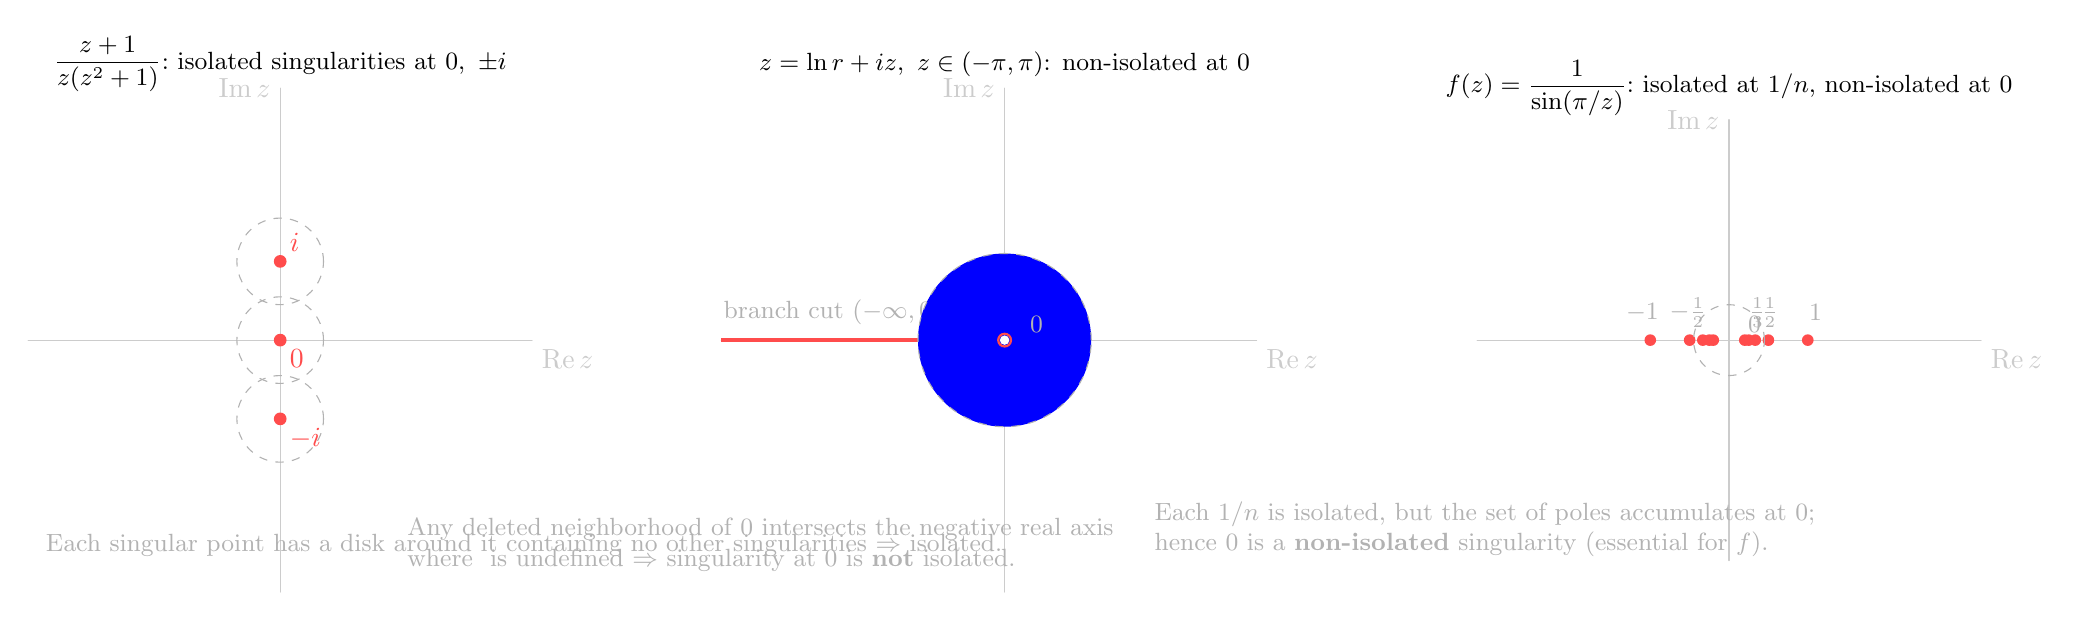
\begin{tikzpicture}[>=Latex,scale=1]
		\tikzset{
			axis/.style={gray!40, line cap=round},
			title/.style={font=\small},
			note/.style={gray!60, font=\small},
			iso/.style={red!70, fill=red!70},              % isolated singularity point
			noniso/.style={red!70, draw=red!70, thick},    % boundary/non-isolated marking
			cut/.style={red!70, very thick},               % branch cut
			domainshade/.style={blue!6},                   % domain shading
			circlethin/.style={draw=gray!60, dashed}
		}
		
		% ========== Panel 1: (z+1)/(z(z^2+1)) — isolated at 0, ±i ==========
		\begin{scope}
			% axes
			\draw[axis] (-3.2,0) -- (3.2,0) node[below right] {$\Re z$};
			\draw[axis] (0,-3.2) -- (0,3.2) node[left] {$\Im z$};
			\node[title] at (0,3.5)
			{$\displaystyle \frac{z+1}{z(z^2+1)}$:$\ \text{isolated singularities at } 0,\ \pm i$};
			
			% points: 0 and ±i
			\fill[iso] (0,0) circle (2.3pt) node[below right] {$0$};
			\fill[iso] (0,1) circle (2.3pt) node[above right] {$i$};
			\fill[iso] (0,-1) circle (2.3pt) node[below right] {$-i$};
			
			% small dashed neighborhoods to emphasize 'isolated'
			\draw[circlethin] (0,0) circle (0.55);
			\draw[circlethin] (0,1) circle (0.55);
			\draw[circlethin] (0,-1) circle (0.55);
			
			\node[note,anchor=west] at (-3.1,-2.6)
			{Each singular point has a disk around it containing no other singularities $\Rightarrow$ isolated.};
		\end{scope}
		
		% ========== Panel 2: principal Log — non-isolated at 0 due to branch cut ==========
		\begin{scope}[xshift=9.2cm]
			% axes
			\draw[axis] (-3.6,0) -- (3.2,0) node[below right] {$\Re z$};
			\draw[axis] (0,-3.2) -- (0,3.2) node[left] {$\Im z$};
			\node[title] at (0,3.5)
			{$\Log z=\ln r + i\Arg z,\ \Arg z\in(-\pi,\pi)$: non-isolated at $0$};
			
			% branch cut on (-∞,0]
			\draw[cut] (-3.6,0) -- (0,0);
			\node[note] at (-2.2,0.35) {branch cut $(-\infty,0]$};
			
			% mark 0 and show any punctured neighborhood meets the cut
			\draw[circlethin,fill=blue] (0,0) circle (1.1);
			\fill[white] (0,0) circle (0.06); % punctured feel (not required but illustrative)
			\draw[noniso] (0,0) circle (2.3pt);
			\node[note,anchor=west] at (0.2,0.2) {$0$};
			
			\node[note,align=left] at (-3.1,-2.6)
			{Any deleted neighborhood of $0$ intersects the negative real axis\\
				where $\Log$ is undefined $\Rightarrow$ singularity at $0$ is \emph{not} isolated.};
		\end{scope}
		
		% ========== Panel 3: 1/sin(π/z) — poles at 1/n accumulating at 0 ==========
		\begin{scope}[xshift=18.4cm]
			% axes
			\draw[axis] (-3.2,0) -- (3.2,0) node[below right] {$\Re z$};
			\draw[axis] (0,-2.8) -- (0,2.8) node[left] {$\Im z$};
			\node[title] at (0,3.2)
			{$\displaystyle f(z)=\frac{1}{\sin(\pi/z)}$:\ isolated at $1/n$, non-isolated at $0$};
			
			% mark poles at z = 1/n on real axis, n = ±1..±5 (schematic)
			\foreach \n in {1,2,3,4,5}{
				\fill[iso] ({1/(\n)},0) circle (2.1pt);
				\fill[iso] ({-1/(\n)},0) circle (2.1pt);
			}
			\node[note] at (1.1,0.35) {$1$};
			\node[note] at (0.52,0.35) {$\frac12$};
			\node[note] at (0.36,0.35) {$\frac13$};
			\node[note] at (-1.1,0.35) {$-1$};
			\node[note] at (-0.52,0.35) {$-\frac12$};
			
			% accumulation at 0
			\draw[circlethin] (0,0) circle (0.45);
			\node[note,anchor=west] at (0.12,0.2) {$0$};
			\node[note,align=left] at (-3.1,-2.4)
			{Each $1/n$ is isolated, but the set of poles accumulates at $0$;\\
				hence $0$ is a \emph{non-isolated} singularity (essential for $f$).};
		\end{scope}
	\end{tikzpicture}
\end{center} 
\end{example}

%\begin{remark}
%	If $f$ is analytic inside a positively oriented simple closed contour $C$ except at finitely many points $z_1,\dots,z_n$, those points are necessarily isolated, and their deleted neighborhoods can be chosen to lie entirely inside $C$. It is also convenient to treat $\infty$ as an isolated singular point when $f$ is analytic for $R_1<|z|<\infty$. 
%\end{remark}
%
%\section{Residues}
%
%\begin{observation}[Laurent expansion near an isolated singularity]
%	If $z_0$ is an isolated singular point, then on $0<|z-z_0|<R$,
%	\[
%	f(z)=\sum_{n=0}^{\infty} a_n (z-z_0)^n+\sum_{n=1}^{\infty}\frac{b_n}{(z-z_0)^n}.
%	\]
%\end{observation}
%
%\begin{definition}[Residue]
%	The coefficient $b_1$ in the Laurent expansion is the \emph{residue} of $f$ at $z_0$:
%	\[
%	\Res_{z=z_0} f=\frac{1}{2\pi i}\int_C f(z)\,dz,
%	\]
%	where $C$ is any positively oriented simple closed contour around $z_0$ lying in the punctured disk. Also,
%	\[
%	\int_C \frac{1}{z-z_0}\,dz=2\pi i,\qquad 
%	\int_C \frac{1}{(z-z_0)^{n+1}}\,dz=0\ (n\ge1).
%	\]
%\end{definition}
%
%\begin{example}\label{ex:z2sin1z}
%	On $|z|=1$,
%	\[
%	\int_{|z|=1} z^2\sin\!\Big(\frac{1}{z}\Big)\,dz
%	=2\pi i\,\Res_{z=0}\Big[z^2\sin\!\Big(\frac{1}{z}\Big)\Big].
%	\]
%	Since $\sin w = w-\frac{w^3}{3!}+\frac{w^5}{5!}-\cdots$, we get
%	\[
%	z^2\sin\!\Big(\frac{1}{z}\Big)=z-\frac{1}{3!z}+\frac{1}{5!z^{3}}-\cdots,
%	\]
%	so the residue is $-1/3!$ and the integral equals $-\dfrac{\pi i}{3}$.
%\end{example}
%
%\begin{example}
%	\[
%	\int_{|z|=1} \exp\!\Big(\frac{1}{z^2}\Big)\,dz=0
%	\]
%	because $\exp(1/z^2)=1+\frac{1}{z^2}+\frac{1}{2!z^4}+\cdots$ has no $1/z$ term.
%\end{example}
%
%\begin{example}
%	Evaluate $\displaystyle \int_{|z-2|=1}\frac{dz}{z(z-2)^4}$. Expanding at $z=2$,
%	\[
%	\frac{1}{z(z-2)^4}
%	=\frac{1}{(z-2)^4}\,\frac{1}{2+(z-2)}
%	=\sum_{n=0}^{\infty}\frac{(-1)^n}{2^{n+1}}(z-2)^{n-4},
%	\]
%	so the residue is the coefficient of $(z-2)^{-1}$, namely $-\frac{1}{16}$. Hence the integral equals $-\,\dfrac{\pi i}{8}$.
%\end{example}
%
%\section{Cauchy’s Residue Theorem}
%
%\begin{theorem}[Residue Theorem]
%	Let $C$ be a positively oriented simple closed contour and assume $f$ is analytic on and inside $C$ except at finitely many isolated singular points $z_1,\dots,z_n$ inside $C$. Then
%	\[
%	\int_C f(z)\,dz=2\pi i\sum_{k=1}^{n}\Res_{z=z_k} f.
%	\]
%\end{theorem}
%
%\begin{example}
%	On $|z|=2$, compute
%	\[
%	\int_C \frac{5z-2}{z(z-1)}\,dz.
%	\]
%	There are simple poles at $0$ and $1$. A quick series check (or the formula in Theorem~\ref{thm:simple-pole-by-quotient} below) gives residues $2$ at $0$ and $3$ at $1$, so the integral equals $2\pi i(2+3)=10\pi i$.
%\end{example}
%
%\subsection*{Residue at infinity}
%If $f$ is analytic in the finite plane except at finitely many singular points inside $C$, then
%\[
%\int_C f(z)\,dz
%=2\pi i\,\Res_{z=0}\!\left[\frac{1}{z^2}\,f\!\Big(\frac{1}{z}\Big)\right].
%\]
%
%\section{The Three Types of Isolated Singular Points}
%
%\begin{definition}[Principal part]
%	In the Laurent expansion at $z_0$, the series $\sum_{n\ge1} b_n/(z-z_0)^n$ is the \emph{principal part}.
%\end{definition}
%
%\begin{definition}[Pole and order]
%	If only finitely many $b_n$ are nonzero, then $z_0$ is a \emph{pole}; if the last nonzero term is $b_m/(z-z_0)^m$ with $m\ge1$, the pole has \emph{order} $m$ (order $1$ = simple pole).
%\end{definition}
%
%\begin{example}
%	$\displaystyle \frac{z^2-2z+3}{z-2}=2+(z-2)+\frac{3}{z-2}$ has a simple pole at $z=2$ with residue $3$. The function $\displaystyle \frac{1}{z^2(1+z)}=\frac{1}{z^2}-\frac{1}{z}+1-\cdots$ has a pole of order $2$ at $0$ with residue $-1$. Also $\displaystyle \frac{\sinh z}{z^4}=\frac{1}{z^3}+\frac{1}{3!z}+\cdots$ has a pole of order $3$ at $0$ and residue $1/6$.
%\end{example}
%
%\begin{definition}[Removable singularity]
%	If all $b_n=0$ (i.e.\ no principal part), then $z_0$ is \emph{removable}. E.g.\ $\displaystyle \frac{1-\cos z}{z^2}=\frac12-\frac{z^2}{4!}+\cdots$ is analytic near $0$ after setting the value $1/2$ at $z=0$.
%\end{definition}
%
%\begin{definition}[Essential singularity]
%	If infinitely many $b_n$ are nonzero, $z_0$ is \emph{essential}. For example, $e^{1/z}=1+\frac1z+\frac1{2!z^2}+\cdots$ has an essential singularity at $0$.
%\end{definition}
%
%\section{Residues at Poles}
%
%\begin{theorem}[Computing residues at poles]\label{thm:pole-phi}
%	An isolated singular point $z_0$ is a pole of order $m$ iff
%	\[
%	f(z)=\frac{\phi(z)}{(z-z_0)^m},
%	\]
%	with $\phi$ analytic and $\phi(z_0)\ne 0$. Then
%	\[
%	\Res_{z=z_0} f=
%	\begin{cases}
%		\phi(z_0), & m=1,\\[3pt]
%		\dfrac{\phi^{(m-1)}(z_0)}{(m-1)!}, & m\ge 2.
%	\end{cases}
%	\]
%\end{theorem}
%
%\begin{example}
%	$\displaystyle f(z)=\frac{z+1}{z^2+9}$ has simple poles at $\pm 3i$. Writing $f(z)=\dfrac{\phi(z)}{z-3i}$ with $\phi(z)=\dfrac{z+1}{z+3i}$, we get $\Res_{z=3i}f=\phi(3i)=\dfrac{3-i}{6}$ and $\Res_{z=-3i}f=\dfrac{3+i}{6}$. 
%\end{example}
%
%\begin{example}
%	For $\displaystyle f(z)=\frac{z^3+2z}{(z-i)^3}$, we have $m=3$ and $\phi(z)=z^3+2z$, so $\Res_{z=i} f=\dfrac{\phi''(i)}{2!}=3i$.
%\end{example}
%
%\begin{example}
%	With the branch $\log z=\ln r+i\theta$ ($r>0$, $0<\theta<2\pi$), the function $\displaystyle f(z)=\frac{(\log z)^3}{z^2+1}$ has a simple pole at $z=i$ and
%	\[
%	\Res_{z=i} f=\frac{(\log z)^3}{z+i}\Bigg|_{z=i}=-\frac{\pi^3}{16}.
%	\]
%\end{example}
%
%\begin{example}
%	Beware misidentification of the order: $\displaystyle \frac{\sinh z}{z^4}$ has order $3$ at $0$, not $4$, because of the series in the previous section; the residue is $1/6$. For $\displaystyle f(z)=\frac{1}{z(e^z-1)}$, one finds a pole of order $2$ at $0$ with $\Res_{z=0} f=-\tfrac12$.
%\end{example}
%
%\section{Zeros of Analytic Functions}
%
%\begin{definition}[Zero of order $m$]
%	If $f$ is analytic at $z_0$, and $f(z_0)=\cdots=f^{(m-1)}(z_0)=0$ but $f^{(m)}(z_0)\ne0$, then $f$ has a \emph{zero of order $m$} at $z_0$; equivalently,
%	\[
%	f(z)=(z-z_0)^m g(z)
%	\]
%	with $g$ analytic and $g(z_0)\ne0$.
%\end{definition}
%
%\begin{example}
%	$f(z)=z(e^z-1)$ has a zero of order $2$ at $z=0$ since $f(0)=f'(0)=0$ and $f''(0)=2\ne0$; writing $f(z)=z^2 g(z)$ defines an entire $g$ with $g(0)=1$.
%\end{example}
%
%\begin{theorem}[Isolated zeros and identity principle]
%	If $f$ is analytic near $z_0$ and not identically zero there, then $f(z)\ne0$ on some punctured neighborhood of $z_0$. If $f$ vanishes on a domain (or a line segment with accumulation in the domain), then $f\equiv0$ on that neighborhood.
%\end{theorem}
%
%\section{Zeros and Poles of a Quotient}
%
%\begin{theorem}\label{thm:quotient-order}
%	Let $p$ and $q$ be analytic at $z_0$, with $p(z_0)\ne0$ and $q$ having a zero of order $m$ at $z_0$. Then $p/q$ has a pole of order $m$ at $z_0$.
%\end{theorem}
%
%\begin{theorem}[Simple pole and residue]\label{thm:simple-pole-by-quotient}
%	If $p,q$ are analytic at $z_0$, $p(z_0)\ne0$, $q(z_0)=0$, and $q'(z_0)\ne0$, then $z_0$ is a simple pole of $p/q$ and
%	\[
%	\Res_{z=z_0}\frac{p(z)}{q(z)}=\frac{p(z_0)}{q'(z_0)}.
%	\]
%\end{theorem}
%
%\begin{example}
%	Let $z_0=1+i$ and $f(z)=\dfrac{z}{z^4+4}$. Since $q(z)=z^4+4$ has a simple zero at $z_0$, 
%	\[
%	\Res_{z=z_0} f=\frac{z_0}{q'(z_0)}=\frac{z_0}{4z_0^3}=\frac{1}{8i}=-\frac{i}{8}.
%	\]
%\end{example}
%
%\section{Behavior Near Isolated Singular Points}
%
%\begin{theorem}
%	If $z_0$ is a pole of $f$, then $\displaystyle \lim_{z\to z_0} f(z)=\infty$.
%\end{theorem}
%
%\begin{theorem}[Riemann’s removable singularity criterion]
%	If $f$ is analytic and bounded on $0<|z-z_0|<\varepsilon$, then either $f$ is analytic at $z_0$ (removable singularity) or can be redefined at $z_0$ to make it analytic.
%\end{theorem}
%
%\begin{theorem}[Casorati--Weierstrass]
%	If $z_0$ is an essential singularity of $f$, then in every deleted neighborhood of $z_0$ the image of $f$ is dense in $\C$ (indeed, arbitrarily close to any $w_0\in\C$).
%\end{theorem}

\newpage
\subsection{Exercises}
\begin{enumerate}[\bf 1.]
	\item %(Residue-theorem evaluations on $|z|=3$)\; 
	Use Cauchy's residue theorem to evaluate integral of each these functions around the circle $|z|=3$ in the positive sense: \[
	\frac{e^{-z}}{z^2},\qquad
	\frac{e^{-z}}{(z-1)^2},\qquad
	z^2 \exp\left(\frac{1}{z}\right),\qquad
	\frac{z+1}{z^2-2z}.
	\] (Answers: $-2\pi i$, $-2\pi i/e$, $\pi i/3$, $2\pi i$.)
	\begin{proof}[\sol]
		All integrals are $\displaystyle \int_{|z|=3} (\cdot)\,d z$ with positive orientation.
		\begin{enumerate}[(1)]
			\item \(\displaystyle \int_{|z|=3} \frac{e^{-z}}{z^2}\,\d z\).\quad
			Let $f(z) = e^{-z}$. Then $f$ is entire (analytic everywhere), and the only
			singularity of the integrand inside $|z|=3$ is a pole of order $2$ at $z=0$.
			By Cauchy's integral formula for the first derivative, 
%			if $f$ is analytic on and inside a simple closed contour $C$ and $z_0$ is interior to $C$, then
			\[
			f'(z_0) = \frac{1}{2\pi i} \int_{|z|=3} \frac{f(z)}{(z - z_0)^2}\,\d z.\implies \int_{|z|=3} \frac{f(z)}{(z - z_0)^2}\,\d z = 2\pi i\, f'(z_0).
			\] With $z_0 = 0$,
			\[
			\int_{|z|=3} \frac{e^{-z}}{z^2}\,\d z = 2\pi i\, f'(0)=2\pi i\cdot \frac{\d}{\d z} e^{-z}\Big|_{z=0}=2\pi i\cdot -e^{-z}\big|_{z=0}=2\pi i\cdot (-1)=-2\pi i.
			\]
			\item \(\displaystyle \int \frac{e^{-z}}{(z-1)^2}\,\d z\).\quad
			Let $f(z) = e^{-z}$, which is entire. The integrand has a pole of order
			$2$ at $z=1$. Since $|1|<3$, this singularity lies inside the circle $|z|=3$,
			and there are no other singularities inside the contour. By Cauchy's integral formula for the first derivative, with $z_0=1$,
			\[
			\int_{|z|=3} \frac{f(z)}{(z-1)^2}\,\d z = 2\pi i\cdot f'(1)=2\pi i\cdot (-e^{-z})\big|_{z=1}=2\pi i\cdot\left(-\frac{1}{e}\right)=\frac{-2\pi i}{e}.
			\]
			\item \(\displaystyle \int_{|z|=3} z^2 \exp\!\left(\frac{1}{z}\right)\,\d z\).\quad
			The only singularity of the integrand is at $z=0$, due to
			the factor $e^{1/z}$. This is an essential singularity at $z=0$, which lies
			inside the contour $|z|=3$. We use the residue theorem:
%			If $f$ has isolated singularities $z_1,\dots,z_n$
%			inside a simple closed contour $C$, and is analytic on $C$, then
			\[
			\int_C f(z)\,dz = 2\pi i \sum_{k=1}^n \operatorname{Res}(f, z_k).
			\]
			Here there is only one singularity at $z=0$, so
			\[
			\int_{|z|=3} z^2 \exp\!\left(\frac{1}{z}\right)\,\d z = 2\pi i \,\operatorname{Res}\!\left(z^2 e^{1/z}, 0\right).
			\]
			To find the residue, expand $\exp\left(\frac{1}{z}\right)$ in a Laurent series around $z=0$:
			\begin{align*}
			\exp\left(\frac{1}{z}\right) &= \sum_{n=0}^\infty \frac{1}{n!}\left(\frac{1}{z}\right)^n
			= 1 + \frac{1}{z} + \frac{1}{2!z^2} + \frac{1}{3!z^3} + \cdots,\\
			z^2 \exp\left(\frac{1}{z}\right)
			&= z^2 \left(1 + \frac{1}{z} + \frac{1}{2!z^2} + \frac{1}{3!z^3} + \cdots\right)\\
			&= z^2 + z + \frac{1}{2!} + \frac{1}{3!}\frac{1}{z} + \frac{1}{4!}\frac{1}{z^2} + \cdots.
			\end{align*} The residue at $z=0$ is $
			\operatorname{Res}\!\left(z^2 e^{1/z},0\right) = \frac{1}{3!} = \frac{1}{6}$. Therefore \[
			\int_{|z|=3} z^2 \exp\!\left(\frac{1}{z}\right)\,\d z = 2\pi i \cdot \frac{1}{6} = \frac{\pi i}{3}.
			\]
			\item \(\displaystyle \int_{|z|=3} \frac{z+1}{z^2-2z}\,\d z=\int \frac{z+1}{z(z-2)}\,\d z\).\quad
			The singularities are simple poles at $z=0$ and $z=2$. 
%			Both of these points satisfy $|z|<3$, hence they lie inside the contour $|z|=3$.
			We can either compute residues directly or use partial fraction decomposition: \begin{align*}
			\frac{z+1}{z(z-2)} = \frac{A}{z} + \frac{B}{z-2} &\implies z+1 = A(z-2) + Bz\\
			&\implies z+1 = (A+B)\,z - 2A\\
			&\implies \begin{cases}
				A + B = 1,\\
				-2A = 1.
			\end{cases}\\
			&\implies A=-1/2\quad\text{and}\quad B=3/2.
			\end{align*} Thus \[
			\frac{z+1}{z^2 - 2z}
			= -\frac{1}{2z} + \frac{3}{2(z-2)}.
			\]
			Now the integral becomes
			\[
			\int \frac{z+1}{z(z-2)}\,\d z = \int_{|z|=3} \left(-\frac{1}{2z} + \frac{3}{2(z-2)}\right)\,dz
			= -\frac{1}{2} \int_{|z|=3} \frac{1}{z}\,dz
			+ \frac{3}{2} \int_{|z|=3} \frac{1}{z-2}\,dz.
			\] Note that \[
			\int_{|z|=3} \frac{1}{z}\,dz = 2\pi i
			\quad\text{and}\quad
			\int_{|z|=3} \frac{1}{z-2}\,dz = 2\pi i,
			\] since both $z=0$ and $z=2$ lie inside $|z|=3$. Therefore
			\[
			\int \frac{z+1}{z(z-2)}\,\d z = -\frac{1}{2} \cdot 2\pi i + \frac{3}{2} \cdot 2\pi i
			= -\pi i + 3\pi i = 2\pi i.
			\]
		\end{enumerate}
	\end{proof}
	\newpage
	\item Show that the singular point of each of the following functions is a pole. \[
	f(z)=\frac{1-\cosh z}{z^3},\quad g(z)=\frac{1-\exp(2z)}{z^4},\quad h(z)=\frac{\exp(2z)}{(z-1)^2}.
	\] Determine the order $m$ of that pole and the corresponding residue $B$.
	
	(Answers: $f(z)$: $m=1$, $B=-1/2$; $g(z)$: $m=3$, $B=-{4}/{3}$; $h(z)$: $m=2$, $B=2e^2$.)
	\begin{proof}[\sol]
		\ \begin{enumerate}[(1)]
			\item $\displaystyle f(z)=\frac{1-\cosh z}{z^3}$ at $z=0$.\quad
			Note that
			\begin{align*}
			\cosh z&=1+\frac{1}{2!}\,z^2+\frac{1}{4!}\,z^4+\frac{1}{6!}\,z^6+\cdots,\\
			1-\cosh z&= -\frac{1}{2}\,z^2-\frac{1}{4!}\,z^4-\frac{1}{6!}\,z^6-\cdots,\\
			\frac{1-\cosh z}{z^3}&= -\frac{1}{2}\,\frac{1}{z}-\frac{1}{4!}\,z+\frac{1}{6!}\,z^3+\cdots.
			\end{align*}
			Hence the singularity is a \emph{simple pole} ($m=1$) with residue $
			B=\Res_{z=0} f = -\frac{1}{2}.$
			\item $\displaystyle g(z)=\frac{1-\exp(2z)}{z^4}$ at $z=0$.
			Note that \begin{align*}
				\exp(2z)&=1+2z+\frac{(2z)^2}{2!}+\frac{(2z)^3}{3!}+\frac{(2z)^4}{4!}+\cdots \\
				&=1+2z+2z^2+\frac{4}{3}z^3+\frac{2}{3}z^4+\cdots,\\
				1-\exp(2z)&= -\Big(2z+2z^2+\frac{4}{3}z^3+\frac{2}{3}z^4+\cdots\Big),\\
				\frac{1-\exp(2z)}{z^4}&= -\frac{2}{z^3}-\frac{2}{z^2}-\frac{4}{3}\,\frac{1}{z}-\frac{2}{3}+\cdots.
			\end{align*} Thus we have a pole of order $3$ ($m=3$) with residue $
			B=\Res_{z=0} g = -\frac{4}{3}.$
			\item $\displaystyle h(z)=\frac{\exp(2)}{(z-1)^2}$ at $z=1$.\quad
			Let $w:=z-1$, i.e., $z=1+w$. Then \begin{align*}
			\exp(2z)&=\exp(2(1+w))=\exp(2)\,\exp(2w)\\
			&=\exp(2)\left(1+2w+\frac{2^2}{2!}w^2+\frac{2^3}{3!}w^3+\cdots\right),\\
			\frac{\exp(2z)}{(z-1)^2}
			&=\frac{\exp(2)}{w^2}\left(1+2w+\frac{2^2}{2!}w^2+\cdots\right)
			=\exp(2)\left(\frac{1}{w^2}+\frac{2}{w}+\frac{2^2}{2!}+\cdots\right).
			\end{align*}
			Therefore the singularity is a pole of order $2$ ($m=2$) with residue $
			B=\Res_{z=1} h = 2\exp(2).$
		\end{enumerate}
	\end{proof}
	\item Show that \begin{align*}
		\Res_{z=-1}\frac{z^{1/4}}{z+1}&=\frac{1+i}{\sqrt2} &(\abs{z}>0,\; 0<\arg z<2\pi),\\
		\Res_{z=i}\frac{\Log\; z}{(z^2+1)^2}&=\frac{\pi+2i}{8},&\\
		\Res_{z=i}\frac{z^{1/2}}{(z^2+1)^2}&=\frac{1-i}{8\sqrt2} &(\abs{z}>0,\; 0<\arg z<2\pi).
	\end{align*}
	\begin{proof}[\sol]
		\ \begin{enumerate}[(1)]
			\item \textbf{(Residue of $f_1(z)=\dfrac{z^{1/4}}{z+1}$ at $z=-1$)}\quad We work with the branch \[
			|z|>0,\quad 0<\arg z<2\pi,
			\] so the branch cut is along the positive real axis, and \[
			z^{1/4} = \exp(\frac14 \Log z),\qquad
			\Log\; z = \ln|z| + i\arg z,\quad 0<\arg z<2\pi.
			\] 	At $z=-1$ we have $|-1|=1$ and $\arg(-1)=\pi$, hence \[
			\Log(-1) = \ln 1 + i\pi = i\pi,
			\] and therefore \[
			z^{1/4}\big|_{z=-1}=(-1)^{1/4} = \exp\left(i\frac{\pi}{4}\right)
			= \cos\frac{\pi}{4} + i\sin\frac{\pi}{4}
			= \frac{1+i}{\sqrt2}.
			\] 	The integrand $\displaystyle f_1(z) = \frac{z^{1/4}}{z+1}$ has a simple pole at $z=-1$, and $z^{1/4}$ is analytic at $z=-1$ on this branch. Consider \[
			g(z):=(z+1)\,f_1(z) = (z+1)\,\frac{z^{1/4}}{z+1} = z^{1/4}.
			\] Since $z^{1/4}$ is analytic at $z=-1$, the function $(z+1)f_1(z)$ is analytic
			at $z=-1$. Therefore it has a Taylor expansion around $z=-1$:
			\[
			(z+1)f_1(z) = z^{1/4}
			= a_0 + a_1(z+1) + a_2(z+1)^2 + \cdots,\quad\text{with}\quad a_n=\frac{g^{(n)}(-1)}{n!}\;(n=0,1,2,\dots),
			\]
			valid for $z$ near $-1$. Dividing both sides by $(z+1)$, we get a Laurent
			expansion for $f_1$ at $z=-1$:
			\[
			f_1(z)
			= \frac{a_0}{z+1} + a_1 + a_2(z+1) + \cdots.
			\]
			By definition, the residue of $f_1$ at $z=-1$ is $
			\Res_{z=-1} f_1(z) = a_0$. Thus \[
			\Res_{z=-1}\frac{z^{1/4}}{z+1}
			=a_0=\frac{g^{(0)}(-1)}{0!}
			= \lim_{z\to-1}(z+1)\frac{z^{1/4}}{z+1}
			= (-1)^{1/4}
			= \frac{1+i}{\sqrt2}.
			\]
%			\begin{center}
%				\begin{tikzpicture}[>=Latex,scale=1]
%					\tikzset{
%						axis/.style={black, line cap=round},
%						cut/.style={orange!85!black, very thick},
%						domain/.style={draw=none, fill=orange!10},
%						pole/.style={red!70, draw=red!70, thick},
%						analpt/.style={blue!65, fill=blue!65},
%						note/.style={gray!60, font=\small},
%						title/.style={font=\small}
%					}
%					
%					% ===================== LEFT: z-plane (branch & pole) =====================
%					\begin{scope}
%						% axes
%						\draw[axis] (-3.4,0) -- (3.6,0) node[right] {$\Re z$};
%						\draw[axis] (0,-2.6) -- (0,2.8) node[above] {$\Im z$};			
%						% branch cut along positive real axis
%						\draw[cut] (0,0) -- (3.4,0);
%						\node[note] at (2.6,0.35) {branch cut};
%						
%						% optional: indicate admissible arguments by two thin rays just above/below the cut
%						\draw[gray!50, dashed] (0,0) -- (3.2,0.18);
%						\draw[gray!50, dashed] (0,0) -- (3.2,-0.18);
%						
%						% the point z = -1
%						\fill[analpt] (-1,0) circle (2.4pt) node[below] {$-1$};
%						% small neighborhood disk showing analyticity of z^{1/4} at -1
%						\draw[blue!65, dashed] (-1,0) circle (0.5);
%						%				\node[note,anchor=west] at (-2.9,-2.2)
%						%				{$\Log z=\ln|z|+i\arg z,\ 0<\arg z<2\pi$;\quad $\arg(-1)=\pi$\\
%							%					$\Log(-1)=i\pi$,\quad $(-1)^{1/4}=e^{\frac14\Log(-1)}=e^{i\pi/4}$};
%						
%						% the function f(z) = z^{1/4}/(z+1) has a simple pole at z=-1
%						\draw[pole] (-1,0) circle (8pt);
%						\node[note] at (-1.1,0.9) {simple pole of $f$ at $-1$};
%						
%						%				% residue computation tag
%						%				\node[note,draw,rounded corners=2pt,fill=gray!5,align=left] at (1.9,1.8)
%						%				{$\displaystyle \Res_{z=-1}\frac{z^{1/4}}{z+1}
%							%					=\lim_{z\to-1}(z+1)\frac{z^{1/4}}{z+1}
%							%					=(-1)^{1/4}=\frac{1+i}{\sqrt2}.$};
%					\end{scope}
%					
%					% ===================== RIGHT: w-plane (value of (-1)^{1/4}) =====================
%					\begin{scope}[xshift=9.2cm]
%						% axes
%						\draw[axis] (-2.4,0) -- (2.6,0) node[below right] {$\Re w$};
%						\draw[axis] (0,-2.4) -- (0,2.6) node[left] {$\Im w$};
%						\node[title] at (0,2.95)
%						{$w=z^{1/4}=e^{\frac14\Log z}$ \quad (value at $z=-1$)};
%						
%						% unit circle
%						\draw[gray!45] (0,0) circle (2.0);
%						
%						% angle arc for pi/4
%						\draw[gray!55,->] (1.3,0) arc[start angle=0,end angle=45,radius=1.3];
%						\node[note] at (1.4,0.5) {$\frac{\pi}{4}$};
%						
%						% point w = e^{i\pi/4} = (cos, sin) = (√2/2, √2/2)
%						\coordinate (W) at (0.7071,0.7071);
%						\fill[blue!65] (W) circle (2.6pt);
%						\draw[gray!55,dashed] (0,0) -- (W);
%						%				\node[note,anchor=west] at (0.78,0.74)
%						%				{$(-1)^{1/4}=e^{i\pi/4}=\dfrac{1+i}{\sqrt2}$};
%					\end{scope}	
%				\end{tikzpicture}
%			\end{center}
			\item \textbf{(Residue of $f_2(z)=\dfrac{\Log z}{(z^2+1)^2}$ at $z=i$)}\quad 
			We factor $z^2+1 = (z-i)(z+i)$, so near $z=i$, \[
			(z^2+1)^2 = (z-i)^2(z+i)^2.
			\]
			Hence \[
			f_2(z) = \frac{\Log z}{(z-i)^2(z+i)^2}
			= \frac{g(z)}{(z-i)^2},\qquad
			g(z) := \frac{\Log z}{(z+i)^2}.
			\]
			The function $g$ is analytic at $z=i$. Thus $z=i$ is a double pole of $f$ of the form $f_2(z) = g(z)/(z-i)^2$ with $g$ analytic at $i$. Then \[
			\Res_{z=i} f_2(z) = \Res_{z=i} \frac{g(z)}{(z-i)^2} = \frac{g^{(1)}(i)}{1!}=g'(i).
			\] Compute $g'(i)$: \begin{align*}
				g'(i)=\frac{d}{dz}g(z)\Bigg|_{z=i}&=\frac{d}{dz}\left((\Log z)(z+i)^{-2}\right)\Bigg|_{z=i}\\
				&=\left[\frac{1}{z}(z+i)^{-2} - 2\Log z\,(z+i)^{-3}\right]_{z=i}\\
				&=\frac{1}{i}\cdot\frac{1}{-4}-2\Log(i)\cdot\frac{1}{-8i}\\
				&=\frac{-1}{4i}+\frac{1}{4i}\cdot(\ln|i|+i\arg(i))\\
				&=\frac{i}{4}+\frac{-i}{4}\cdot\left(0+\frac{\pi i}{2}\right)\\
				&=\frac{2i}{8}+\frac{\pi}{8}\\
				&=\frac{\pi+2i}{8}.
			\end{align*}
			\item \textbf{(Residue of $f_3(z)=\dfrac{z^{1/2}}{(z^2+1)^2}$ at $z=i$)}\quad
			As before, $
			(z^2+1)^2 = (z-i)^2(z+i)^2,$
			so \[
			f_3(z) = \frac{z^{1/2}}{(z-i)^2(z+i)^2}
			= \frac{h(z)}{(z-i)^2},\qquad
			h(z) := \frac{z^{1/2}}{(z+i)^2},
			\] and $h(z)$ is analytic at $z=i$. Thus $z=i$ is again a double pole of $f_3$, and $\Res_{z=i} f(z) = h'(i).$ Compute $h'(i)$: \begin{align*}
				h'(i)=\frac{d}{dz}h(z)\Bigg|_{z=i}&=\frac{d}{dz}\left(z^{1/2}(z+i)^{-2}\right)\Bigg|_{z=i}\\
				&=\left[ \frac{1}{2} z^{-1/2}(z+i)^{-2} - 2 z^{1/2}(z+i)^{-3}\right]_{z=i}\\
				&=\frac{1}{2}\cdot i^{-1/2}\cdot\frac{1}{-4}-2\cdot i^{1/2}\cdot\frac{1}{-8i}.
			\end{align*}
			We need the branch values of $z^{1/2}$ and $z^{-1/2}$ at $z=i$ for $0<\arg z<2\pi$: \begin{align*}
			i^{1/2} &= \exp(\frac12\Log i)
			= \exp(\frac12 (\ln|i|+i\arg(i)))
			= \exp(\frac12 \left(\frac{\pi i}{2}\right))
			= \exp(i\pi/4)
			= \cos\frac{\pi}{4} + i\sin\frac{\pi}{4}
			= \frac{1+i}{\sqrt2},\\
			i^{-1/2} &= \frac{1}{i^{1/2}}
			=\frac{1}{\frac{1+i}{\sqrt{2}}}
			= \frac{\sqrt2}{1+i}
			= \frac{\sqrt2(1-i)}{(1+i)(1-i)}
			= \frac{\sqrt2(1-i)}{2}
			= \frac{1-i}{\sqrt2}.
			\end{align*}
			Therefore \begin{align*}
				h'(i)&=\frac{1}{2}\cdot i^{-1/2}\cdot\frac{1}{-4}-2\cdot i^{1/2}\cdot\frac{1}{-8i}\\
				&=\frac{-1}{8}\left(\frac{1-i}{\sqrt{2}}\right)+\frac{-i}{4}\left(\frac{1+i}{\sqrt{2}}\right)\\
				&=\frac{-(1-i)+2(1-i)}{8\sqrt{2}} \\
				&=\frac{(1-i)}{8\sqrt{2}}
			\end{align*}
			Thus
			\[
			\Res_{z=i}\frac{z^{1/2}}{(z^2+1)^2}
			= h'(i)
			= \frac{1-i}{8\sqrt2}.
			\]
		\end{enumerate}
	\end{proof}
	\newpage
	\item Find the value of the integral \[
	\int_{|z|=3}\frac{z^3\,e^{1/z}}{1+z^3}\,dz
	\] taken CCW around the circle $\abs{z}=3$. 
	
	(Answer: $2\pi i$.)
	\begin{proof}[\sol]
	Let \[
	f(z) = \frac{z^3 e^{1/z}}{1+z^3}.
	\] Set
	\[
	w = \frac{1}{z} \quad\Longrightarrow\quad z = \frac{1}{w},\quad dz = -\frac{1}{w^2}\,dw.
	\] The circle $|z| = 3$ corresponds to $|w| = 1/3$. As $z$ runs CCW, $w=1/z$ runs clockwise. Therefore,
	\begin{align*}
		\int_{|z|=3} f(z)\,dz
		&= \underbrace{\int_{\substack{|w|=1/3}} 	f\!\left(\frac{1}{w}\right)\left(-\frac{1}{w^2}\,dw\right)}_{\text{CW}}\\
		&= \underbrace{-\int_{\substack{|w|=1/3}} 	f\!\left(\frac{1}{w}\right)\left(-\frac{1}{w^2}\,dw\right)}_{\text{CCW}}\\
		&= \int_{|w|=1/3} \frac{f(1/w)}{w^2}\,dw.
	\end{align*}
	Since \[
	f\!\left(\frac{1}{w}\right)
	= \frac{(1/w)^3 e^{w}}{1 + (1/w)^3}
	= \frac{\frac{e^w}{w^3}}{\frac{w^3 + 1}{w^3}}
	= \frac{e^w}{w^3+1},
	\] we have \[
	\int_{|z|=3} f(z)\,dz=\int_{|w|=1/3} \left(\frac{1}{w^2}\cdot f\left(\frac{1}{w}\right)\right)\,dw
	=\int_{|w|=1/3} \frac{e^w}{w^2(w^3+1)}\,dw.
	\]
	The only singularity of
	\[
	h(w) = \frac{e^w}{w^2(w^3+1)}
	\]
	inside the circle $|w|=1/3$ is at $w=0$, since the roots of $w^3+1=0$ are
	\[
	w=-1,\quad w=e^{i\pi/3},\quad w=e^{-i\pi/3},
	\]
	all of which satisfy $|w|=1$. Hence, by the residue theorem,
	\[
	\int_{|z|=3} f(z)\,dz = 2\pi i \,\Res_{w=0} h(w).
	\]
	We compute the residue via series expansion. Write \[
	h(w) = \frac{1}{w^2}\cdot \frac{e^w}{1+w^3}.
	\] Since \begin{align*}
		\frac{1}{1+w^3} &= 1 - w^3 + w^6 - w^9 + \cdots \quad (|w|<1)\quad\text{and} \\
		e^w &= 1 + w + \frac{w^2}{2} + \frac{w^3}{6} + \cdots,
	\end{align*} we have
	\[
	\frac{e^w}{1+w^3}
	= (1 + w + \frac{w^2}{2} + \frac{w^3}{6} + \cdots)(1 - w^3 + w^6 - \cdots),
	\] and so \begin{align*}
		h(w) &= \frac{1}{w^2}\cdot \left(\left(1 + w + \frac{w^2}{2} + \frac{w^3}{6} + \cdots\right)(1 - w^3 + w^6 - \cdots)\right)\\
		&=\frac{1}{w^2}\left(\left(1 + w + \frac{w^2}{2} + \frac{w^3}{6} + \cdots\right)-
		\left(w^3 + w^4 + \frac{w^5}{2} + \frac{w^6}{6} + \cdots\right)+
		\left(w^6 + w^7 + \frac{w^8}{2} + \frac{w^9}{6} + \cdots\right)
		-\cdots\right)\\
		&=\left(\frac{1}{w^2} + {\color{red}\frac{1}{w}} + \frac{1}{2} + \frac{w}{6} + \cdots\right)-
		\left(w^1 + w^2 + \frac{w^3}{2} + \frac{w^4}{6} + \cdots\right)+
		\left(w^4 + w^5 + \frac{w^6}{2} + \frac{w^7}{6} + \cdots\right)
		-\cdots.
	\end{align*}
	Thus $\Res_{w=0} h(w) = 1$. By the residue theorem, \[
	\int_{|z|=3}\frac{z^3 e^{1/z}}{1+z^3}\,dz = 2\pi i \,\Res_{w=0} h(w) = 2\pi i \cdot 1 = 2\pi i.
	\]
	\end{proof}
	\newpage
	\item Let $C$ denote the positively oriented circle $|z|=2$. Show that \[
	\int_C \tan z\,dz=-4\pi i\quad\text{and}\quad\int_C \frac{dz}{\sinh 2z}=-\pi i.
	\]
	\begin{proof}[\sol]
	\ \begin{enumerate}[(1)]
		\item We have $\displaystyle\tan z = \frac{\sin z}{\cos z}$. The poles of $\tan z$ are the zeros of $\cos z$, i.e.,
		\[
		\cos z = 0 \iff z = \frac{\pi}{2} + k\pi,\quad k\in\mathbb{Z}.
		\]
		We need those with $|z|<2$. Numerically,
		\[
		\left|\frac{\pi}{2}\right| \approx 1.57 < 2,\quad
		\left|-\frac{\pi}{2}\right| \approx 1.57 < 2,
		\]
		while $\bigl|\frac{3\pi}{2}\bigr| > 2$, etc.
		So the poles inside $|z|=2$ are $
		z = \pm\frac{\pi}{2}$. These are simple poles. For a simple pole of a quotient $f/g$ with $g(z_0)=0$, $g'(z_0)\neq 0$,
		\[
		\Res_{z=z_0}\tan z=\Res_{z=z_0} \frac{f(z)}{g(z)} =\lim\limits_{z\to z_0}(z-z_0)\frac{f(z)}{g(z)}
		=\lim\limits_{z\to z_0}\frac{f(z)}{\frac{g(z)}{(z-z_0)}}= \frac{f(z_0)}{g'(z_0)}.
		\]
		Here $f(z)=\sin z$, $g(z)=\cos z$, so $g'(z)=-\sin z$. Then \begin{align*}
			\Res_{z=\frac{\pi}{2}} \tan z
			&= \frac{\sin(\pi/2)}{\cos'(\pi/2)}
			= \frac{1}{-\,\sin(\pi/2)}
			= \frac{1}{-1} = -1\\
			\Res_{z=-\frac{\pi}{2}} \tan z
			&= \frac{\sin(-\pi/2)}{\cos'(-\pi/2)}
			= \frac{-1}{-\,\sin(-\pi/2)}
			= \frac{-1}{1}
			= -1.
		\end{align*}
		So the sum of residues inside $C$ is
		\[
		\Res_{z=\pi/2}\tan z + \Res_{z=-\pi/2}\tan z
		= -1 + (-1) = -2.
		\]
		By the residue theorem,
		\[
		\int_C \tan z\,dz
		= 2\pi i \sum \Res(\tan z)
		= 2\pi i \cdot (-2)
		= -4\pi i.
		\]
		\item Now consider $\displaystyle
		\int_C \frac{dz}{\sinh 2z}$. The poles occur where
		\[
		\sinh 2z = 0.
		\]
		Recall $\sinh w = 0 \iff w = n\pi i$, $n\in\mathbb{Z}$. Thus
		\[
		\sinh 2z = 0 \iff 2z = n\pi i \iff z = \frac{n\pi i}{2},\quad n\in\mathbb{Z}.
		\]
		We need those with $|z|<2$. We have
		\[
		\left|\frac{n\pi i}{2}\right| = \frac{|n|\pi}{2} < 2
		\quad\Longrightarrow\quad |n| < \frac{4}{\pi}\approx 1.27,
		\]
		so the only possibilities are $n = 0, \pm 1$. Hence the poles inside $|z|=2$ are
		\[
		z = 0,\quad z = \pm\frac{\pi i}{2}.
		\]
		These are simple zeros of $\sinh 2z$, since $
		\frac{d}{dz}(\sinh 2z) = 2\cosh 2z$ and $\cosh 2z \neq 0$ at these points.
		We write
		\[
		f(z) = \frac{1}{\sinh 2z} = \frac{1}{h(z)},\quad h(z)=\sinh 2z.
		\]
		For a simple zero $h(z_0)=0$ with $h'(z_0)\neq 0$, the residue of $1/h(z)$ is
		\[
		\Res_{z=z_0} \frac{1}{h(z)} = \frac{1}{h'(z_0)}.
		\]
		Here $h'(z) = 2\cosh 2z$, so
		\[
		\Res_{z=z_0} \frac{1}{\sinh 2z} = \frac{1}{2\cosh 2z_0}.
		\]
		
		\subsection*{Residue at $z=0$}
		\[
		\Res_{z=0} \frac{1}{\sinh 2z}
		= \frac{1}{2\cosh 0}
		= \frac{1}{2\cdot 1}
		= \frac{1}{2}.
		\]
		
		\subsection*{Residue at $z=\frac{\pi i}{2}$}
		Here $2z = \pi i$:
		\[
		\cosh(\pi i) = \cos \pi = -1,
		\]
		so
		\[
		\Res_{z=\frac{\pi i}{2}} \frac{1}{\sinh 2z}
		= \frac{1}{2\cosh \pi i}
		= \frac{1}{2(-1)} = -\frac{1}{2}.
		\]
		
		\subsection*{Residue at $z=-\frac{\pi i}{2}$}
		Here $2z = -\pi i$:
		\[
		\cosh(-\pi i) = \cosh(\pi i) = \cos \pi = -1,
		\]
		so
		\[
		\Res_{z=-\frac{\pi i}{2}} \frac{1}{\sinh 2z}
		= \frac{1}{2\cosh(-\pi i)}
		= \frac{1}{2(-1)}
		= -\frac{1}{2}.
		\]
		
		\subsection*{Sum of residues and the integral}
		
		The sum of residues inside $|z|=2$ is
		\[
		\frac{1}{2} - \frac{1}{2} - \frac{1}{2} = -\frac{1}{2}.
		\]
		
		By the residue theorem,
		\[
		\int_C \frac{dz}{\sinh 2z}
		= 2\pi i \sum \Res\left(\frac{1}{\sinh 2z}\right)
		= 2\pi i \cdot \left(-\frac{1}{2}\right)
		= -\pi i.
		\]
		
		\[
		\boxed{\displaystyle \int_C \frac{dz}{\sinh 2z} = -\pi i.}
		\]
	\end{enumerate}
	\end{proof}
\end{enumerate}

%\vspace{1em}
%\noindent\textbf{Source.} Adapted from the provided lecture note \emph{Complex Variables and Applications — Chapter 6: Residues and Poles}. :contentReference[oaicite:0]{index=0}




\end{document}
